% ============================================================================
% LAKE WAIKARE DIGITAL LIBRARY - MAIN DOCUMENT
% ============================================================================
% Rubric-optimized structure for maximum marks (36/36 points)
% TODO: Copy your main.tex content here
% ============================================================================

% Add your complete main.tex content here

\documentclass[12pt,a4paper]{article}
\usepackage[utf8]{inputenc}
\usepackage[english]{babel}
\usepackage{amsmath,amsfonts,amssymb}
\usepackage{graphicx}
\usepackage{float}
\usepackage{hyperref}
\usepackage{geometry}
\usepackage{fancyhdr}
\usepackage{setspace}
\usepackage{titlesec}
\usepackage{tocloft}
\usepackage{caption}
\usepackage{subcaption}
\usepackage{booktabs}
\usepackage{longtable}
\usepackage{array}
\usepackage{multirow}
\usepackage{xcolor}
\usepackage{listings}
\usepackage{tikz}

% Fix header height warning
\setlength{\headheight}{14.5pt}

% Page setup
\geometry{margin=2.5cm}
\onehalfspacing

% Header and footer
\pagestyle{fancy}
\fancyhf{}
\fancyhead[L]{Lake Waikare Digital Library}
\fancyhead[R]{Final Project Report}
\fancyfoot[C]{\thepage}

% Hyperref setup
\hypersetup{
    colorlinks=true,
    linkcolor=blue,
    filecolor=magenta,      
    urlcolor=cyan,
    citecolor=green,
}

% Title formatting
\titleformat{\section}{\Large\bfseries}{\thesection}{1em}{}
\titleformat{\subsection}{\large\bfseries}{\thesubsection}{1em}{}
\titleformat{\subsubsection}{\normalsize\bfseries}{\thesubsubsection}{1em}{}

% Custom commands
\newcommand{\projecttitle}{Lake Waikare Digital Library: A Cultural and Environmental Preservation Platform}
\newcommand{\course}{CSMAX570-25A}
\newcommand{\group}{Group 10}
\newcommand{\university}{The University of Waikato}

% Placeholder command for images
\newcommand{\placeholder}[4][0.8]{
    \begin{tikzpicture}
        \draw[thick, dashed, gray] (0,0) rectangle (#1\textwidth,#2cm);
        \node[align=center] at (#1\textwidth/2,#2cm/2) {
            \textbf{\large [PLACEHOLDER]}\\[0.5cm]
            \textbf{#3}\\[0.2cm]
            \textit{#4}
        };
    \end{tikzpicture}
}

% Document begins
\begin{document}

\begin{titlepage}
\begin{center}
\vspace*{0.5cm}

% University of Waikato logo

\includegraphics[width=0.3\textwidth]{university_logo.png}\\[1cm]

\textsc{\LARGE The University of Waikato}\\[0.5cm]
\textsc{\Large CSMAX570-25A: Computer Science Masters}\\[1.5cm]

\rule{\linewidth}{0.5mm}\\[0.4cm]
{\huge\bfseries Lake Waikare Digital Library: A Cultural and Environmental Preservation Platform}\\[0.4cm]
\rule{\linewidth}{0.5mm}\\[1cm]

{\Large\bfseries Final Project Report}\\[2cm]

\begin{minipage}{\textwidth}
\begin{center} \large
\emph{Submitted by:}\\[0.5cm]
\begin{tabular}{ll}
GOROKHOVSKAII Joseph & (1048854)\\
LI Chen & (1672194)\\
RAVICHANDRAN Pranavkrishnan & (1660319)\\
LIN Hina & (1646541)\\
\end{tabular}
\end{center}
\end{minipage}\\[1.5cm]

\begin{minipage}{\textwidth}
\begin{center} \large
\emph{Supervision Team:}\\[0.5cm]
\begin{tabular}{l}
Dr. Colin Pilbrow (Project Supervisor)\\
Dr. David Bainbridge (Program Coordinator)\\
Dr. Alvin Yeo (Course Instructor)\\
\end{tabular}
\end{center}
\end{minipage}\\[1.5cm]

{\large Submission Date: Thursday, 29 May 2025}\\[0.5cm]

{\large Group 10}\\[1cm]

\vfill

% Footer with cultural acknowledgment
{\small \emph{Developed in partnership with the Lake Waikare community and local iwi}}

\end{center}
\end{titlepage}


% RUBRIC SECTION 1: ABSTRACT/EXECUTIVE SUMMARY (Weight: 1)
% ================================================================
\newpage
\begin{abstract}
\textbf{\large EXECUTIVE SUMMARY}
\vspace{0.5cm}

The Lake Waikare Digital Library represents a comprehensive digital preservation platform designed to safeguard the cultural heritage and environmental history of the Lake Waikare region in New Zealand. This report presents the final outcomes of an innovative solution that addresses the critical intersection of Māori cultural preservation and environmental awareness through community-centered technology development.

\textbf{Project Essence:} The platform integrates interactive mapping technology, authentic multilingual content presentation (te reo Māori and English), and innovative age-appropriate learning interfaces to serve diverse community needs while respecting traditional knowledge protocols.

\textbf{Key Innovations:} Our primary contribution is the development of a dedicated Child Mode for engaging younger generations with cultural heritage, sophisticated search and filtering capabilities preserving cultural context, and a culturally-sensitive design approach developed through extensive community consultation with cultural authorities.

\textbf{Methodology:} We employed iterative, user-centered design principles with continuous stakeholder feedback integration, prioritizing authentic community partnership over extractive research approaches. The development process integrated ongoing cultural consultation rather than one-time approval mechanisms.

\textbf{Results:} The final prototype demonstrates successful achievement of three primary objectives: effective cultural preservation mechanisms maintaining traditional knowledge integrity, enhanced environmental awareness capabilities connecting cultural and ecological understanding, and inclusive community engagement features supporting intergenerational learning.

\textbf{Impact and Contribution:} This project contributes to digital heritage preservation by demonstrating practical approaches to indigenous knowledge representation, intergenerational cultural transmission, and the integration of environmental education with cultural preservation while maintaining community control and cultural authenticity.

\textbf{Keywords:} Digital heritage preservation, Māori cultural authenticity, Environmental education integration, Intergenerational engagement, Community-centered design, Indigenous knowledge systems, Accessibility and inclusion
\end{abstract}

% Table of Contents
\newpage
\tableofcontents

% List of Figures
\newpage
\listoffigures

% List of Tables
\newpage
\listoftables

% RUBRIC SECTION 2: INTRODUCTION (Weight: 1)
% ==========================================
\newpage
\section*{SECTION 1: PROJECT INTRODUCTION AND CONTEXT}
\addcontentsline{toc}{section}{SECTION 1: PROJECT INTRODUCTION AND CONTEXT}
\section{PROJECT INTRODUCTION AND CONTEXT}

Lake Waikare, situated in the lower Waikato catchment of New Zealand, represents far more than a geographical feature—it embodies centuries of M\=aori cultural heritage, traditional ecological knowledge, and environmental stewardship that has sustained local communities for generations. However, contemporary environmental challenges threaten not only the lake's ecological integrity but also the cultural continuity of the knowledge systems intrinsically connected to this vital natural resource.

\subsection{Cultural and Environmental Crisis}

The environmental degradation of Lake Waikare due to agricultural runoff and inadequate wastewater management has created a cascading effect that extends beyond water quality metrics into the realm of cultural preservation. As the largest shallow lake in the lower Waikato catchment, Lake Waikare has historically served as a cornerstone for M\=aori communities, providing essential resources for sustenance and maintaining profound spiritual and cultural significance \cite{regional_council_2024}. The deterioration of this ecosystem has resulted in the gradual erosion of traditional knowledge, oral histories, and customary practices that have been transmitted through generations.

This phenomenon represents a critical intersection of environmental and cultural loss, where ecological degradation directly threatens the preservation of indigenous knowledge systems. The disconnection between younger generations and their cultural heritage, exacerbated by modernization processes, compounds this challenge by creating knowledge gaps that traditional transmission methods struggle to bridge effectively.

\subsection{Digital Preservation as Cultural Revitalization}

In response to these interconnected challenges, this project investigates the potential of digital technologies to serve as culturally appropriate preservation and revitalization tools. Unlike conventional digital archiving approaches that often treat cultural content as static artifacts, our research explores how interactive digital platforms can maintain the dynamic, relational, and contextual nature of M\=aori knowledge systems while ensuring accessibility for diverse community stakeholders.

The Lake Waikare Digital Library project leverages the Greenstone Digital Library Software as its foundational platform, recognizing Greenstone's established capabilities in cultural heritage preservation and its extensive deployment in indigenous communities worldwide \cite{greenstone_2024}. Developed by the New Zealand Digital Library Project at the University of Waikato, Greenstone provides a robust, open-source framework specifically designed for building and distributing digital library collections, making it particularly suitable for community-controlled cultural preservation initiatives.

The project emerges from extensive community consultation and represents a collaborative effort between academic researchers, local iwi, and community stakeholders to develop a preservation platform that respects traditional knowledge protocols while leveraging Greenstone's proven digital capabilities. This approach recognizes that effective cultural preservation requires more than mere documentation—it demands the creation of engaging, accessible, and culturally authentic platforms that can facilitate intergenerational knowledge transmission while maintaining the technical reliability and scalability that Greenstone provides.

\subsection{Research Significance and Innovation}

This project contributes to the growing field of digital heritage preservation by addressing several critical gaps in existing approaches while demonstrating innovative applications of the Greenstone Digital Library framework. By building upon Greenstone's established architecture, the project explores how existing digital library technologies can be enhanced and customized to serve indigenous knowledge preservation requirements more effectively.

First, the project demonstrates how Greenstone's flexible collection management system can be adapted to respect and reflect indigenous epistemologies rather than imposing Western knowledge organization systems. The platform's customizable interface capabilities enable the creation of culturally appropriate navigation structures and content presentation methods that align with M\=aori knowledge organization principles.

Second, it explores innovative approaches to intergenerational engagement through the development of specialized Child Mode interfaces within the Greenstone framework, demonstrating how established digital library platforms can be extended to make cultural content accessible to younger audiences without compromising authenticity or cultural protocols. This represents a novel application of Greenstone's interface customization capabilities for age-specific cultural engagement.

The integration of environmental and cultural preservation within a single Greenstone-based platform represents an innovative approach that recognizes the inseparable connection between ecological health and cultural vitality in M\=aori worldviews. By leveraging Greenstone's multimedia handling capabilities and metadata management systems, the platform presents environmental data alongside cultural narratives, demonstrating how digital library technologies can support holistic preservation approaches that inform contemporary environmental stewardship while maintaining cultural relevance for modern communities.

\subsection{Community-Centered Methodology}

Central to this project's approach is the recognition that authentic cultural preservation cannot occur without genuine community partnership and ongoing stakeholder engagement. The project operates under the guidance of Glen Tupuhi, our principal stakeholder and cultural authority, whose extensive governance experience and deep cultural connections provide essential direction for the platform's development.

Glen Tupuhi brings unparalleled expertise to this initiative through his role as Trustee of Whakatupu Aotearoa Foundation and his extensive background in M\=aori governance structures. His whakapapa connections—Tainui te waka, Ng\=aati P\=aoa ki Waiheke, T\=amaki Makaurau, Hauraki, Waikato, Ngati Hine, Ngati Naho o Waikato, Ngati Rangimahora, Ng\=aati Apakura—establish direct cultural authority over the Lake Waikare region and ensure that the digital library development respects appropriate cultural protocols and community priorities.

Glen's governance portfolio, including his roles as Hauraki representative for Waikato District Health Board Iwi M\=aori Council, Chair of Ng\=aa Muka Development Trust, and his previous positions with The Ngati P\=aoa Trust and Hauraki M\=aori Trust Board, demonstrates the collaborative networks essential for sustainable cultural preservation initiatives. His academic credentials, including a Graduate Diploma in Business Studies from Massey University and NZ Institute of Directors Certificate, provide the strategic oversight necessary for developing community-controlled digital resources.

Rather than adopting extractive research methodologies that treat communities as data sources, this project employs a collaborative framework where Glen Tupuhi and associated community members serve as co-researchers, cultural authorities, and primary beneficiaries of the developed platform. This methodology ensures that the digital library reflects community priorities, respects cultural protocols, and addresses genuine community needs rather than academic assumptions about cultural preservation requirements.

The involvement of Glen's extensive network, including connections to the Waikato Regional Council through his various trustee roles, demonstrates the project's commitment to creating sustainable, community-controlled resources that can continue to evolve and expand beyond the initial development phase.

\subsection{Project Scope and Objectives}

The Lake Waikare Digital Library project encompasses the design, development, and evaluation of a comprehensive digital platform built upon the Greenstone Digital Library Software framework. This foundation provides the technical infrastructure necessary to serve multiple community stakeholder groups while maintaining cultural authenticity, accessibility, and long-term sustainability.

The platform leverages Greenstone's core capabilities—including multimedia collection management, flexible metadata schemas, and customizable user interfaces—while extending these features through innovative adaptations for cultural preservation and community engagement. The project integrates interactive mapping technologies with Greenstone's search and browsing capabilities, implements multilingual content presentation using Greenstone's internationalization features, and develops sophisticated filtering systems that respect cultural organization principles.

The development of the specialized Child Mode represents a significant extension of Greenstone's interface capabilities, demonstrating how established digital library platforms can be enhanced to create age-appropriate cultural engagement tools while maintaining the robust collection management and preservation standards for which Greenstone is recognized.

This report presents the complete development process, from initial community consultation through final prototype evaluation, demonstrating how the Greenstone platform can be adapted and extended to address community-identified challenges while maintaining rigorous technical standards. The project's outcomes extend beyond the specific Lake Waikare context to provide insights and methodologies applicable to similar Greenstone-based digital heritage preservation initiatives in indigenous communities worldwide, contributing to the broader ecosystem of culturally responsive digital library implementations.

% RUBRIC SECTION 3: COMPANY BACKGROUND/WORK ENVIRONMENT (Weight: 1)
% ================================================================
\newpage
\section*{SECTION 2: ORGANIZATIONAL CONTEXT AND WORK ENVIRONMENT}
\addcontentsline{toc}{section}{SECTION 2: ORGANIZATIONAL CONTEXT AND WORK ENVIRONMENT}
% ============================================================================
% SECTION 2: Organizational Context and Work Environment (Rubric: Company Background - Weight 1)
% ============================================================================
% TODO: Add your content here
% This file maps to the rubric-optimized report structure
% ============================================================================

% Add your LaTeX content below this line
\section{ORGANIZATIONAL CONTEXT AND WORK ENVIRONMENT}

The Lake Waikare Digital Library project operates within a complex multi-organizational ecosystem that reflects the collaborative nature of contemporary indigenous digital heritage initiatives. This section delineates the organizational structures, stakeholder relationships, and institutional frameworks that have shaped the project's development trajectory and ensured its alignment with both academic rigor and community authenticity.

\subsection{Primary Institutional Framework}

\subsubsection{The University of Waikato - Academic Foundation}

The University of Waikato serves as the primary institutional host for this initiative through the CSMAX570-25A Computer Science Masters Extended Programme. The university's established commitment to M\=aori scholarship and digital innovation provides both the academic infrastructure and cultural sensitivity necessary for this type of community-partnered research.

The university's significance extends beyond mere institutional affiliation—it represents the birthplace of the Greenstone Digital Library Software, making it uniquely positioned to support advanced applications of this platform for indigenous cultural preservation. The university's Digital Library Research Group, established in 1995, has maintained continuous development of Greenstone and accumulated extensive expertise in digital heritage applications, particularly within New Zealand's bicultural context \cite{witten_2000}.

The academic supervision structure includes Dr. Colin Pilbrow as Project Supervisor, providing specialized expertise in digital systems development and community-engaged research methodologies. David Bainbridge, serving as Program Coordinator, brings extensive technical knowledge of digital library architectures and has been instrumental in Greenstone's ongoing development. Alvin Yeo, as Course Instructor, ensures that the project meets rigorous academic standards while maintaining practical applicability.

\subsubsection{Supervision and Academic Governance}

The project operates under a robust academic governance structure designed to balance scholarly rigor with community responsiveness. The supervision team represents complementary expertise areas essential for successful digital heritage initiatives:

\textbf{Dr. Colin Pilbrow} provides project oversight with particular emphasis on research methodology, stakeholder engagement protocols, and ensuring that academic outputs serve genuine community needs rather than extractive research purposes. His supervision ensures that the project contributes meaningfully to both academic knowledge and community capacity building.

\textbf{David Bainbridge} contributes technical leadership, particularly regarding Greenstone platform optimization, digital collection management best practices, and long-term sustainability considerations for community-controlled digital resources. His involvement ensures that technical implementations align with established digital library standards while accommodating specific indigenous knowledge organization requirements.

\textbf{Alvin Yeo} maintains academic quality assurance, ensuring that project deliverables meet masters-level research standards while remaining accessible and actionable for community stakeholders. His role includes facilitating connections between theoretical frameworks and practical implementation outcomes.

\subsection{Community Stakeholder Organizations}

\subsubsection{Primary Cultural Authority - Glen Tupuhi and Associated Networks}

Glen Tupuhi represents the project's primary cultural stakeholder, bringing extensive governance experience and deep whakapapa connections that establish authentic community authority over the initiative's direction and implementation. His organizational affiliations create a comprehensive network of cultural and administrative support essential for sustainable digital preservation initiatives.

As Trustee of \textbf{Whakatupu Aotearoa Foundation}, Glen provides direct access to organizational structures specifically designed for M\=aori community development and cultural preservation. This foundation's mission aligns closely with the digital library's objectives, creating natural synergies for long-term platform sustainability and community adoption.

Glen's role as \textbf{Hauraki representative for Waikato District Health Board Iwi M\=aori Council} establishes crucial connections between the digital library initiative and broader regional development strategies, ensuring that cultural preservation efforts integrate with existing community health and wellness frameworks.

His position as \textbf{Chair of Ng\=aa Muka Development Trust}, representing a cluster of northern Waikato marae under Waikato Tainui, provides direct access to the marae network essential for authentic cultural content validation and community engagement. This connection ensures that the digital library reflects genuine community priorities rather than external assumptions about cultural preservation needs.

\subsubsection{Regional Government Partnership}

The \textbf{Waikato Regional Council} serves as a crucial institutional partner, providing both environmental data access and regulatory context essential for the platform's integrated approach to cultural and environmental preservation. The Council's involvement ensures that environmental information presented through the digital library maintains scientific accuracy while supporting traditional ecological knowledge perspectives.

This partnership reflects the Council's recognition that effective environmental management requires integration of indigenous knowledge systems alongside Western scientific approaches. The Council's commitment to Treaty of Waitangi obligations creates a supportive policy environment for initiatives that strengthen M\=aori cultural capacity while addressing environmental challenges.

\subsubsection{Local Iwi Partnership Structure}

The project operates within a broader \textbf{Local Iwi Partnership} framework that ensures authentic community control over cultural content and knowledge sharing protocols. This partnership structure reflects established best practices for indigenous digital heritage initiatives, where community ownership and control remain paramount throughout development and implementation phases.

The iwi partnership provides essential cultural oversight, including validation of content authenticity, approval of knowledge sharing protocols, and ongoing guidance regarding appropriate cultural representation within digital contexts. This relationship ensures that the platform serves community-defined objectives rather than external research agendas.

\subsection{Collaborative Work Environment and Methodology}

\subsubsection{Agile Development Framework}

The project team adopted an agile development methodology specifically adapted for community-engaged digital heritage work. This approach emphasizes iterative development cycles with continuous stakeholder feedback integration, ensuring that technical development remains responsive to evolving community needs and cultural requirements.

Biweekly team meetings provided regular opportunities for progress assessment, challenge identification, and collaborative problem-solving. These meetings included both technical development discussions and cultural consultation processes, ensuring that technological decisions remained grounded in community priorities and cultural appropriateness.

The agile framework proved particularly valuable for managing the complex intersection of technical requirements, academic standards, and cultural protocols. By maintaining flexibility in development approaches while adhering to clear project objectives, the team successfully navigated challenges that traditional project management methodologies might have struggled to accommodate.

\subsubsection{Community Consultation Integration}

Rather than treating community consultation as a discrete project phase, the work environment integrated ongoing stakeholder engagement throughout the development process. This approach reflects recognition that authentic cultural preservation requires continuous community input rather than one-time approval mechanisms.

Regular consultation sessions with Glen Tupuhi and associated community networks provided essential guidance on cultural representation, knowledge organization principles, and appropriate technology applications. These sessions ensured that technical capabilities served community-defined objectives while maintaining cultural integrity and authenticity.

\subsection{Institutional Resources and Infrastructure}

\subsubsection{Technical Infrastructure}

The University of Waikato provided comprehensive technical infrastructure supporting both development activities and long-term platform sustainability. Access to Greenstone development environments, digital collection management systems, and specialized software tools enabled sophisticated prototype development while maintaining alignment with established digital library standards.

The university's commitment to open-source digital library development created an ideal environment for community-controlled resource creation, ensuring that resulting platforms could be maintained and modified by community stakeholders rather than requiring ongoing dependency on external technical expertise.

\subsubsection{Academic and Cultural Resources}

The project benefited from the university's extensive collection of M\=aori scholarship, digital heritage research, and community-engaged research methodologies. Access to specialized libraries, research databases, and expert consultation provided essential background knowledge for culturally appropriate digital platform development.

The university's established relationships with M\=aori communities and commitment to Treaty of Waitangi obligations created a supportive institutional environment for authentic partnership development and culturally responsive research practices.

\subsection{Quality Assurance and Ethical Framework}

The organizational context includes robust quality assurance mechanisms ensuring that academic rigor and cultural authenticity remain complementary rather than competing priorities. Ethics approval processes, cultural consultation protocols, and academic supervision structures work collaboratively to maintain both scholarly standards and community trust.

Regular evaluation processes, including formal presentation opportunities and peer review mechanisms, provide external validation of both technical achievements and cultural appropriateness. These processes ensure that project outcomes contribute meaningfully to both academic knowledge and community capacity while maintaining the highest standards of cultural respect and authenticity.



% RUBRIC SECTION 4: PROJECT DESCRIPTION (Weight: 2)
% =================================================
\newpage
\section*{SECTION 3: PROJECT DESCRIPTION AND BACKGROUND KNOWLEDGE}
\addcontentsline{toc}{section}{SECTION 3: PROJECT DESCRIPTION AND BACKGROUND KNOWLEDGE}

\subsection*{3.1 Literature Review and Background Knowledge}
\addcontentsline{toc}{subsection}{3.1 Literature Review and Background Knowledge}
% ============================================================================
% SECTION 3.1: Literature Review and Background Knowledge (Rubric: Project Description - Weight 2)
% ============================================================================
% TODO: Add your content here
% This file maps to the rubric-optimized report structure
% ============================================================================

% Add your LaTeX content below this line



\subsection*{3.2 Project Goals and Objectives}
\addcontentsline{toc}{subsection}{3.2 Project Goals and Objectives}
% ============================================================================
% SECTION 3.2: Project Goals and Objectives (Rubric: Project Description - Weight 2)
% ============================================================================
% TODO: Add your content here
% This file maps to the rubric-optimized report structure
% ============================================================================

% Add your LaTeX content below this line



\subsection*{3.3 Development Methodology and Project Milestones}
\addcontentsline{toc}{subsection}{3.3 Development Methodology and Project Milestones}
% ============================================================================
% SECTION 3.3: Development Methodology and Project Milestones (Rubric: Project Description - Weight 2)
% ============================================================================
% TODO: Add your content here
% This file maps to the rubric-optimized report structure
% ============================================================================

% Add your LaTeX content below this line



\subsection*{3.4 Requirements Analysis and System Design}
\addcontentsline{toc}{subsection}{3.4 Requirements Analysis and System Design}
% ============================================================================
% SECTION 3.4: Requirements Analysis and System Design (Rubric: Project Description - Weight 2)
% ============================================================================
% TODO: Add your content here
% This file maps to the rubric-optimized report structure
% ============================================================================

% Add your LaTeX content below this line

\section{Requirements Analysis}
\label{sec:requirements}

\subsection{Requirements Gathering Process}
\label{subsec:requirements_process}

The requirements analysis for the Lake Waikare Digital Library employed a comprehensive approach combining stakeholder consultation, cultural research, and technical feasibility assessment. This process ensured that both explicit functional needs and implicit cultural requirements were identified and integrated into the platform specification, with particular emphasis on community data sovereignty and authentic cultural representation.

Requirements gathering occurred through multiple channels: direct stakeholder interviews with Glen Tupuhi and academic supervisors, analysis of existing digital heritage platforms, literature review of indigenous knowledge preservation best practices, evaluation of Greenstone Digital Library capabilities, assessment of Waikato Regional Council environmental data systems, and iterative feedback collection throughout the development process.

The requirements were categorized into functional requirements (what the system must do), non-functional requirements (how the system must perform), cultural requirements (how the system must respect and represent M\=aori values and protocols), technical architecture requirements (how the system integrates with Greenstone), data sovereignty requirements (how community control is maintained), and integration requirements (how external data sources are incorporated).

\subsection{Technical Architecture Requirements}
\label{subsec:technical_architecture}

\subsubsection{Greenstone Platform Integration}
\label{subsubsec:greenstone_integration}

\textbf{TR-01: Core Greenstone Functionality Extension}
\begin{itemize}
    \item The system shall extend Greenstone Digital Library Software core functionality while maintaining compatibility with future Greenstone updates
    \item Custom collection configurations shall follow Greenstone best practices and documentation standards
    \item All customizations shall be implemented through Greenstone's plugin architecture where possible
    \item The system shall preserve Greenstone's administrative interfaces for community management
\end{itemize}

\textbf{TR-02: Metadata Schema Integration}
\begin{itemize}
    \item Custom metadata schemas shall integrate with Greenstone's existing Dublin Core and qualified Dublin Core frameworks
    \item Cultural metadata fields shall be implemented through Greenstone's extensible metadata system
    \item Geographic metadata shall utilize Greenstone's spatial data handling capabilities
    \item Temporal metadata shall support both Western date formats and M\=aori seasonal/cultural time references
\end{itemize}

\textbf{TR-03: Interface Customization Framework}
\begin{itemize}
    \item Child Mode interface shall be implemented through Greenstone's interface customization system
    \item Multilingual support shall utilize Greenstone's internationalization framework
    \item Custom navigation elements shall integrate with Greenstone's existing user interface components
    \item Map integration shall extend Greenstone's spatial browsing capabilities
\end{itemize}

\subsubsection{Community Technical Sustainability}
\label{subsubsec:technical_sustainability}

\textbf{TR-04: Community Maintenance Capability}
\begin{itemize}
    \item All technical implementations shall be documented for community maintenance
    \item Community stakeholders shall receive training in Greenstone administration
    \item Custom code shall follow clear documentation and commenting standards
    \item System architecture shall minimize dependency on external technical expertise
\end{itemize}

\subsection{Data Sovereignty Requirements}
\label{subsec:data_sovereignty}

\subsubsection{Community Data Control}
\label{subsubsec:community_control}

\textbf{DS-01: Indigenous Data Sovereignty Implementation}
\begin{itemize}
    \item All cultural data shall remain under community ownership and control as defined by CARE Principles for Indigenous Data Governance
    \item Community stakeholders shall maintain administrative privileges over all cultural content
    \item Data export capabilities shall enable complete community data portability without technical barriers
    \item No cultural data shall be accessible without appropriate community authorization
\end{itemize}

\textbf{DS-02: Community Governance Integration}
\begin{itemize}
    \item Technical systems shall support community-defined governance structures for content approval
    \item Cultural validation workflows shall be implemented through community-controlled processes
    \item Administrative interfaces shall reflect M\=aori governance principles and decision-making structures
    \item Community authorities shall have technical override capabilities for all content decisions
\end{itemize}

\textbf{DS-03: Cultural Intellectual Property Protection}
\begin{itemize}
    \item Traditional Knowledge Licenses shall be implemented for appropriate cultural content
    \item Cultural attribution shall be maintained through persistent metadata
    \item Community consent mechanisms shall be technically enforced for sensitive content access
    \item Unauthorized reproduction prevention measures shall be implemented where culturally appropriate
\end{itemize}

\subsection{Environmental Data Integration Requirements}
\label{subsec:environmental_integration}

\subsubsection{Regional Council Data Integration}
\label{subsubsec:regional_data}

\textbf{IR-01: Waikato Regional Council Systems Integration}
\begin{itemize}
    \item The system shall integrate with Waikato Regional Council environmental monitoring databases
    \item Water quality data shall be presented with appropriate scientific accuracy and cultural context
    \item Environmental monitoring locations shall be mapped to culturally significant sites where appropriate
    \item Data update frequencies shall maintain currency with Regional Council monitoring schedules
\end{itemize}

\textbf{IR-02: Environmental-Cultural Data Correlation}
\begin{itemize}
    \item Environmental data visualization shall support both Western scientific and M\=aori knowledge perspectives
    \item Historical environmental data shall correlate with cultural timeline information and oral histories
    \item Environmental change indicators shall be presented alongside cultural impact narratives
    \item Traditional ecological knowledge shall be integrated with scientific environmental data where appropriate
\end{itemize}

\subsection{Functional Requirements}
\label{subsec:functional_requirements}

\subsubsection{Core Platform Functionality}
\label{subsubsec:core_functionality}

\textbf{FR-01: Content Management and Organization}
\begin{itemize}
    \item The system shall support multiple content types including text, images, audio, video, and environmental data
    \item The system shall organize content into Records, Collections, Trails, and Overlays following Greenstone collection management principles
    \item The system shall maintain hierarchical content relationships and cross-references through Greenstone's relationship management
    \item The system shall support content versioning and historical tracking with full audit trails
\end{itemize}

\textbf{FR-02: Search and Discovery}
\begin{itemize}
    \item The system shall provide comprehensive search functionality across all content using Greenstone's search architecture
    \item The system shall support filtering by content type, category, date range, geographic location, and cultural significance
    \item The system shall enable both simple keyword search and advanced multi-criteria search with cultural category support
    \item The system shall provide search suggestions and auto-completion functionality in both English and te reo M\=aori
\end{itemize}

\textbf{FR-03: Geographic Information Integration}
\begin{itemize}
    \item The system shall display content on an interactive map interface integrated with Greenstone's spatial browsing
    \item The system shall support multiple map layers for cultural heritage, environmental data, and historical information
    \item The system shall enable geographic filtering and location-based content discovery with cultural site recognition
    \item The system shall integrate satellite, topographic, and traditional M\=aori spatial representation methods
\end{itemize}

\textbf{FR-04: Culturally-Responsive Interface Adaptability}
\begin{itemize}
    \item The system shall provide separate Adult and Child interface modes with culturally appropriate design elements
    \item The system shall support seamless switching between interface modes without data loss
    \item The system shall adapt interface elements based on cultural protocols and user preferences
    \item The system shall maintain functionality across different interface modes while respecting cultural access restrictions
\end{itemize}

\subsubsection{Content Presentation Requirements}
\label{subsubsec:content_presentation}

\textbf{FR-05: Multilingual and Cultural Support}
\begin{itemize}
    \item The system shall support both English and te reo M\=aori content presentation with te reo M\=aori prioritized
    \item The system shall enable seamless language switching without data loss or cultural context loss
    \item The system shall maintain cultural context and appropriate cultural terminology across language presentations
    \item The system shall support te reo M\=aori screen reader compatibility and accessibility tools
\end{itemize}

\textbf{FR-06: Multimedia Integration}
\begin{itemize}
    \item The system shall support audio narration for accessibility and traditional oral history preservation
    \item The system shall integrate video content with appropriate cultural context and accessibility features
    \item The system shall optimize multimedia content for varying connection speeds common in rural communities
    \item The system shall provide alternative formats for accessibility compliance and cultural transmission methods
\end{itemize}

\textbf{FR-07: Interactive and Cultural Features}
\begin{itemize}
    \item The system shall provide contextual information through culturally appropriate popup interfaces
    \item The system shall support user navigation through related content using M\=aori knowledge organization principles
    \item The system shall enable appropriate content sharing and referencing functionality with cultural attribution
    \item The system shall provide educational activities and interactive elements in Child Mode that maintain cultural authenticity
\end{itemize}

\subsubsection{Data Management Requirements}
\label{subsubsec:data_management}

\textbf{FR-08: Cultural Content Categorization}
\begin{itemize}
    \item The system shall organize content into thematic categories reflecting M\=aori knowledge organization (M\=aori History, Environmental Knowledge, etc.)
    \item The system shall support temporal categorization using both Western and M\=aori seasonal/cultural time references
    \item The system shall enable content tagging and metadata assignment following cultural protocols
    \item The system shall maintain category relationships and hierarchies that respect M\=aori epistemological structures
\end{itemize}

\textbf{FR-09: Integrated Data Management}
\begin{itemize}
    \item The system shall integrate environmental monitoring data with appropriate cultural context and interpretation
    \item The system shall support historical data visualization that correlates environmental and cultural changes
    \item The system shall enable data export for research and educational purposes while maintaining cultural protocols
    \item The system shall maintain data accuracy, source attribution, and cultural acknowledgment for all content
\end{itemize}

\subsection{Non-Functional Requirements}
\label{subsec:nonfunctional_requirements}

\subsubsection{Performance Requirements}
\label{subsubsec:performance_requirements}

\textbf{NFR-01: Community-Appropriate System Performance}
\begin{itemize}
    \item Page load times shall be optimized for rural internet connectivity commonly available in the Lake Waikare region
    \item Map interface shall support smooth interaction on devices commonly used by community members
    \item Search results shall be returned within reasonable timeframes considering community network conditions
    \item The system shall support concurrent access by community groups and educational sessions without degradation
\end{itemize}

\textbf{NFR-02: Scalability for Community Growth}
\begin{itemize}
    \item The system architecture shall support content expansion as community contributions grow
    \item The system shall accommodate increasing user engagement through sustainable scaling approaches
    \item Data storage shall support growing content volumes efficiently within community resource constraints
    \item Interface components shall adapt to increased content without compromising cultural presentation quality
\end{itemize}

\subsubsection{Compatibility Requirements}
\label{subsubsec:compatibility_requirements}

\textbf{NFR-03: Community Technology Compatibility}
\begin{itemize}
    \item The system shall function consistently across web browsers commonly used by community members
    \item The system shall provide responsive design supporting devices accessible to diverse community demographics
    \item The system shall maintain functionality across different operating systems without requiring software purchases
    \item The system shall support both high-speed urban and limited rural bandwidth connections effectively
\end{itemize}

\textbf{NFR-04: Inclusive Device Accessibility}
\begin{itemize}
    \item The system shall support older devices within community members' economic reach
    \item The system shall provide interfaces appropriate for users with varying technological experience
    \item The system shall maintain functionality across different screen sizes including older mobile devices
    \item The system shall support both touch and traditional input methods without preference
\end{itemize}

\subsubsection{Security and Privacy Requirements}
\label{subsubsec:security_requirements}

\textbf{NFR-05: Cultural Data Security}
\begin{itemize}
    \item The system shall protect cultural content according to traditional knowledge protocols and community-defined access levels
    \item The system shall implement secure data transmission and storage that maintains community control
    \item The system shall maintain comprehensive audit trails for all cultural content access and modifications
    \item The system shall respect indigenous intellectual property rights and cultural ownership through technical enforcement
\end{itemize}

\textbf{NFR-06: Community Privacy Protection}
\begin{itemize}
    \item The system shall not collect personal information without explicit, informed community consent
    \item The system shall provide transparent privacy policies developed with community input and approval
    \item The system shall enable community control over all data collection and usage practices
    \item The system shall comply with relevant privacy legislation while prioritizing indigenous data sovereignty principles
\end{itemize}

\subsection{Cultural Requirements}
\label{subsec:cultural_requirements}

\subsubsection{Cultural Authenticity and Protocol Requirements}
\label{subsubsec:cultural_authenticity}

\textbf{CR-01: M\=aori Cultural Protocol Technical Implementation}
\begin{itemize}
    \item The system shall implement technical mechanisms for traditional knowledge access restrictions based on cultural protocols
    \item The system shall maintain cultural ownership acknowledgment through persistent, tamper-proof metadata
    \item The system shall integrate traditional M\=aori design principles through culturally-validated interface elements
    \item The system shall maintain cultural context and significance through specialized metadata schemas and presentation methods
\end{itemize}

\textbf{CR-02: Community Authority and Validation Systems}
\begin{itemize}
    \item All cultural content shall be validated through technically-supported community authority workflows
    \item The system design shall incorporate real-time community feedback and guidance mechanisms
    \item Cultural representation shall be subject to community approval through integrated validation systems
    \item The system shall support community involvement in content development through user-friendly contribution tools
\end{itemize}

\subsubsection{Cultural Preservation and Transmission Requirements}
\label{subsubsec:cultural_preservation}

\textbf{CR-03: Traditional Knowledge Technical Preservation}
\begin{itemize}
    \item The system shall preserve traditional knowledge using culturally appropriate digital formats and presentation methods
    \item The system shall maintain technical connections between cultural practices and environmental knowledge through linked data structures
    \item The system shall support intergenerational knowledge transmission through age-appropriate but culturally consistent interfaces
    \item The system shall technically enforce appropriate access controls for sacred or sensitive cultural information
\end{itemize}

\textbf{CR-04: Cultural Education Technical Support}
\begin{itemize}
    \item The system shall provide educational resources through technically sophisticated but culturally appropriate delivery methods
    \item The system shall support both formal and informal cultural learning through flexible content presentation systems
    \item The system shall integrate cultural values and worldviews throughout the technical platform architecture
    \item The system shall promote understanding of cultural and environmental connections through sophisticated data correlation and presentation
\end{itemize}

\subsection{Accessibility Requirements}
\label{subsec:accessibility_requirements}

\subsubsection{Cultural and Universal Design Requirements}
\label{subsubsec:cultural_universal_design}

\textbf{AR-01: Culturally-Informed Accessibility Compliance}
\begin{itemize}
    \item The system shall meet WCAG 2.1 Level AA accessibility standards while accommodating M\=aori cultural interface preferences
    \item All interactive elements shall be keyboard accessible and compatible with te reo M\=aori screen readers
    \item Color contrast and visual design shall meet accessibility requirements while respecting M\=aori aesthetic principles
    \item Alternative text and multimedia descriptions shall maintain cultural context and appropriate cultural terminology
\end{itemize}

\textbf{AR-02: Community-Specific Assistive Technology Support}
\begin{itemize}
    \item The system shall be compatible with assistive technologies used by community members
    \item The system shall provide audio descriptions that maintain cultural context and te reo M\=aori pronunciation
    \item The system shall support interface modifications appropriate for elder users and varying visual capabilities
    \item The system shall enable navigation methods suitable for users with varying technological experience
\end{itemize}

\subsubsection{Community Inclusive Design Requirements}
\label{subsubsec:community_inclusive_design}

\textbf{AR-03: Multi-Generational Community Accessibility}
\begin{itemize}
    \item The system shall accommodate community members with varying technical skills through progressive interface complexity
    \item Interface complexity shall be adjustable based on user preferences while maintaining cultural authenticity
    \item The system shall provide multiple pathways to access content reflecting different learning and discovery styles
    \item Help and guidance shall be available throughout the user experience in both English and te reo M\=aori
\end{itemize}

\textbf{AR-04: Economic and Digital Equity}
\begin{itemize}
    \item The system shall be freely accessible without cost barriers to community members
    \item The system shall function effectively on older devices within community members' economic reach
    \item Content shall be optimized for minimal data usage to accommodate limited internet plans
    \item The system shall not require premium software, subscriptions, or additional purchases for full functionality
\end{itemize}

\subsection{User Story Analysis}
\label{subsec:user_stories}

\subsubsection{Primary Community User Stories}
\label{subsubsec:primary_stories}

\textbf{US-01: Cultural Knowledge Keeper (Kaumatua)}
``As an elder with traditional knowledge about Lake Waikare, I want to share cultural stories and practices with younger generations through a digital platform that respects our cultural protocols, maintains the integrity of our traditional knowledge, and ensures our stories remain under our control.''

\textbf{Acceptance Criteria:}
\begin{itemize}
    \item Cultural content can be contributed through community-controlled validation processes
    \item Traditional knowledge is presented with proper cultural context and protocol compliance
    \item Content accessibility accommodates elders with varying technical experience
    \item Cultural ownership and intellectual property rights are technically enforced and clearly acknowledged
    \item Sacred or sensitive knowledge can be restricted according to traditional protocols
\end{itemize}

\textbf{US-02: M\=aori Educator}
``As a teacher working in M\=aori education, I want to access authentic cultural materials and environmental education resources about Lake Waikare that I can integrate into my curriculum while maintaining cultural authenticity and supporting student connection to their heritage.''

\textbf{Acceptance Criteria:}
\begin{itemize}
    \item Educational resources are organized according to both Western curriculum needs and M\=aori knowledge structures
    \item Content is validated by cultural authorities and maintains authenticity
    \item Materials can be easily integrated into existing educational frameworks
    \item Age-appropriate content maintains cultural significance without oversimplification
    \item Environmental and cultural connections are clearly presented for educational use
\end{itemize}

\textbf{US-03: Community Member with Whakapapa Connections}
``As a community member with whakapapa connections to Lake Waikare, I want to explore the cultural and environmental heritage of this place to strengthen my understanding of my cultural identity and my responsibilities as tangata whenua.''

\textbf{Acceptance Criteria:}
\begin{itemize}
    \item Content is accessible through both geographic and cultural navigation methods
    \item Whakapapa and cultural connections are clearly presented and maintained
    \item Historical and contemporary information integrates cultural and environmental perspectives
    \item Personal cultural exploration is supported through respectful, intuitive interfaces
    \item Community contributions and perspectives are prominently featured
\end{itemize}

\subsubsection{Intergenerational User Stories}
\label{subsubsec:intergenerational_stories}

\textbf{US-04: Tamariki Learner}
``As a child learning about my M\=aori heritage, I want to explore Lake Waikare's stories and environmental importance through engaging activities that help me understand my culture and my responsibility to protect our environment.''

\textbf{Acceptance Criteria:}
\begin{itemize}
    \item Child Mode interface is culturally appropriate and developmentally suitable
    \item Content is presented through interactive activities that maintain cultural authenticity
    \item Cultural information is accessible and engaging without compromising traditional knowledge integrity
    \item Environmental education integrates M\=aori worldview and Western science appropriately
    \item Learning progression supports different cultural learning styles and capabilities
\end{itemize}

\textbf{US-05: Whanau Learning}
``As a parent wanting to strengthen our family's cultural connections, I want to explore cultural and environmental information about Lake Waikare with my children to support intergenerational learning and cultural transmission within our wh\=anau.''

\textbf{Acceptance Criteria:}
\begin{itemize}
    \item Platform supports shared exploration and intergenerational discussion
    \item Content is appropriate for wh\=anau learning and cultural transmission
    \item Interface modes accommodate both adult and child users seamlessly
    \item Cultural protocols for knowledge sharing within families are supported
    \item Learning resources support parents in cultural teaching roles
\end{itemize}

\subsubsection{External User Stories}
\label{subsubsec:external_stories}

\textbf{US-06: Respectful Researcher}
``As a researcher studying indigenous knowledge systems and environmental management, I want to access well-documented cultural and environmental information about Lake Waikare for my academic work while respecting cultural protocols, acknowledging community ownership, and ensuring my research benefits the community.''

\textbf{Acceptance Criteria:}
\begin{itemize}
    \item Advanced search capabilities support detailed research while respecting access protocols
    \item Content is properly documented with metadata that maintains cultural context and attribution
    \item Cultural protocols and access restrictions are clearly indicated and technically enforced
    \item Research use requires appropriate cultural permissions and community benefit agreements
    \item Data can be referenced and cited in ways that respect indigenous intellectual property
\end{itemize}

\subsection{Requirements Prioritization}
\label{subsec:requirements_prioritization}

Requirements were prioritized using the MoSCoW method (Must have, Should have, Could have, Won't have) in direct consultation with Glen Tupuhi and community stakeholders, with cultural authenticity and community control prioritized above technical sophistication:

\subsubsection{Must Have Requirements}
\label{subsubsec:must_have}

\begin{table}[H]
\centering
\caption{Must Have Requirements Priority Matrix}
\label{tab:must_have_requirements}
\begin{tabular}{@{}ll@{}}
\toprule
\textbf{Requirement Category} & \textbf{Critical Requirements} \\
\midrule
Data Sovereignty & Community control, cultural IP protection \\
Cultural Authenticity & Community validation, protocol compliance \\
Technical Foundation & Greenstone integration, basic functionality \\
Accessibility & Community device support, multilingual interface \\
Core Functionality & Content management, search, geographic integration \\
\bottomrule
\end{tabular}
\end{table}

\subsubsection{Should Have Requirements}
\label{subsubsec:should_have}

\begin{itemize}
    \item Advanced environmental data visualization with cultural context
    \item Comprehensive Child Mode educational activities
    \item Enhanced community contribution and validation workflows
    \item Sophisticated cultural-environmental data correlation tools
    \item Advanced accessibility features for diverse community needs
\end{itemize}

\subsubsection{Could Have Requirements}
\label{subsubsec:could_have}

\begin{itemize}
    \item Enhanced multimedia optimization for very limited bandwidth
    \item Integration with external M\=aori educational platforms
    \item Advanced data export capabilities for research purposes
    \item Community-controlled social features for knowledge sharing
\end{itemize}

\subsubsection{Won't Have Requirements (This Phase)}
\label{subsubsec:wont_have}

\begin{itemize}
    \item Mobile application development (web-first approach prioritized)
    \item Virtual reality integration (technology access barriers for community)
    \item Advanced gamification features (potential cultural appropriateness concerns)
    \item Commercial features or revenue generation capabilities
\end{itemize}

\subsection{Requirements Validation}
\label{subsec:requirements_validation}

Requirements validation occurred through multiple culturally-appropriate mechanisms throughout the project lifecycle, with community authority and cultural authenticity prioritized over technical validation:

\subsubsection{Cultural Authority Validation Process}
\label{subsubsec:cultural_validation}

Cultural requirements were validated through ongoing consultation with Glen Tupuhi and associated cultural authorities, ensuring that platform development respected traditional protocols, community values, and indigenous data sovereignty principles. This validation process included review of technical implementations for cultural appropriateness, assessment of community control mechanisms, and evaluation of cultural representation accuracy.

\subsubsection{Community Stakeholder Review Process}
\label{subsubsec:community_stakeholder_review}

Regular consultation with community stakeholders ensured requirements remained aligned with genuine community needs rather than external assumptions about cultural preservation. Bi-weekly review sessions provided opportunities for requirement refinement, cultural protocol clarification, and community priority validation.

\subsubsection{Technical Feasibility Assessment}
\label{subsubsec:technical_feasibility}

Technical requirements were validated through Greenstone platform assessment, prototype development, and testing with community-accessible devices and network conditions. This ensured that functional specifications could be implemented within community technical contexts and resource constraints while maintaining cultural requirement compliance.

\subsubsection{Academic Supervision Validation}
\label{subsubsec:academic_validation}

Academic supervisors provided validation of requirement comprehensiveness, technical feasibility, and project scope appropriateness while ensuring that academic rigor supported rather than compromised community objectives and cultural authenticity.

The comprehensive requirements analysis provided a culturally-grounded foundation for platform development, ensuring that both explicit functional needs and implicit cultural considerations were addressed throughout the design and implementation process. This approach prioritizes community data sovereignty and cultural authenticity while leveraging sophisticated technical capabilities to serve genuine community needs.

% RUBRIC SECTION 5: PROJECT RESULTS (Weight: 2)
% =============================================
\newpage
\section*{SECTION 4: PROJECT EXECUTION AND RESULTS}
\addcontentsline{toc}{section}{SECTION 4: PROJECT EXECUTION AND RESULTS}

\subsection*{4.1 Technical Implementation and Execution}
\addcontentsline{toc}{subsection}{4.1 Technical Implementation and Execution}
% ============================================================================
% SECTION 4.1: Technical Implementation and Execution (Rubric: Project Results - Weight 2)
% ============================================================================
% TODO: Add your content here
% This file maps to the rubric-optimized report structure
% ============================================================================

% Add your LaTeX content below this line

% ============================================================================
% SECTION 4.1: Technical Implementation and Execution (Rubric: Project Results - Weight 2)
% ============================================================================

\subsection{Technical Implementation and Execution}

\subsubsection{Wireframe Integration and Design Adjustments}

The development of the prototype was based on the wireframe design previously discussed and documented. Overall, we retained the core structure established in the earlier wireframe, including the homepage layout, the sidebar’s basic structure and animation, the Māori language toggle, the map feature, the main search functionality, and the children’s mode.

However, several structural and functional adjustments were made in response to supervisor feedback and our own hands-on experience with the wireframe.

Firstly, we added an onboarding guide to the homepage. During initial use, users may find it difficult to fully understand or discover all available features on the homepage. The onboarding guide helps users become familiar with key functions, thereby improving the overall user experience.

Secondly, the language toggle now defaults to Māori instead of English, as originally designed in the wireframe. This change reflects the intended user base and emphasizes the website’s commitment to Māori cultural preservation.

Thirdly, we reordered the sidebar, moving the search feature to the bottom. This adjustment groups all map-related features together for better usability and task flow.

Additionally, we enhanced the map interactivity by allowing users to view detailed information about selected locations. This builds on the interactive map foundation while offering deeper insight into location-specific content.

In the children’s mode, we revised the exit logic, allowing users to more easily return to the main site. This improves the usability of the children’s experience.

Lastly, we added a backend administration module, which includes features for adding new records and managing existing ones. This module is critical for content control, data entry, and permission management—functions essential for a system similar to a digital library.

\subsubsection{From Figma to Code-Based Prototyping}

In the early stages of wireframing and prototyping, we used Figma as our primary tool. Figma is widely used for early-stage design and prototyping due to its rich design elements, transition animations, and built-in presentation mode. Its collaborative features also allowed us to work together online in real time, which greatly facilitated team coordination during the initial development phase.

However, as the prototype grew in complexity, we encountered increasing difficulties in managing changes within Figma. Adding new features or modifying existing ones often required significant rework across multiple components, making the development process inefficient. Additionally, inconsistent implementation of interactions and animations by different team members led to frequent errors and omissions.

To address these issues and improve both flexibility and presentation quality, we decided to shift to a code-based approach using HTML, CSS, JavaScript, and http-server. Compared to Figma, this approach allowed greater control over the layout, behavior, and animations, while still supporting all visual and interactive features we needed. The use of http-server enabled smooth local previewing with basic routing and language switching support. Moreover, developing with HTML allowed us to embed our final presentation content directly into the prototype itself, creating a seamless demo experience without the need to switch between slides and prototype.

For the interactive map component, we used the Leaflet library, which enabled rich map interactions, including location markers, pop-up details, and customized styling—fully meeting our prototype’s mapping requirements.

Overall, the team collaboratively selected tools, designed reusable components, and implemented the final prototype through discussion and iteration. This process not only improved the quality of the final product but also deepened our understanding of frontend technologies and system architecture.

\subsubsection{Team Collaboration and Technical Implementation}

The successful delivery of our prototype relied heavily on effective team collaboration. To simulate a professional working environment, we utilized Microsoft Teams for communication and GitHub for version control, aligning with standard practices in contemporary software development. These tools enabled structured coordination and efficient collaboration throughout the project lifecycle.

Weekly retrospectives were conducted every Wednesday morning, during which we reviewed our progress, identified and addressed technical challenges, and established goals for the subsequent development phases. These sessions ensured alignment with the course timeline and facilitated continuous improvement. Beyond formal meetings, our group maintained regular communication via Teams to support ongoing coordination and issue resolution.

Each team member assumed distinct responsibilities and contributed meaningfully to the project. Hina managed the overall timeline and was primarily responsible for the design and development of the map module, including its interactive elements. Joseph, as team leader, oversaw the structural organization of the prototype, led the homepage development, and contributed to the final presentation design. Pranav focused on the development of the administrative interface and proposed essential backend features, including access control mechanisms. Chen Li was responsible for the implementation of the search functionality and the design and development of the Children’s Mode—a feature designed to enhance accessibility and support Māori cultural preservation.

The project followed a structured development plan from inception to completion. In Week 4, we participated in a requirements elicitation session with Glen Tupuhi to define core goals. Week 5 focused on requirement analysis and conceptual modeling. In Week 6, initial sketches and conceptual evaluations were developed. Between Weeks 7 and 9, we created and refined low-fidelity mockups based on peer and supervisor feedback, before progressing to wireframes. From Week 10 onward, these wireframes were iteratively translated into a functional prototype. Weeks 11 to 13 were dedicated to the implementation of core modules—including the homepage, map, search, Children’s Mode, and admin panel—followed by the integration of the final presentation directly into the prototype. The development remained on schedule due to coordinated team effort.

Several technical strategies were employed to enhance usability. To support new users, we implemented a guided tour using the Bootstrap Tour library. The tour highlights key interface components through contextual instructions and is triggered conditionally based on a localStorage flag to avoid redundancy on repeat visits. For the exit mechanism in Children’s Mode, we designed a custom JavaScript-based confirmation process to prevent unintentional navigation, involving a floating action button with an embedded verification popup and session tracking.

The map module, serving as the system’s central interactive component, was developed using the Leaflet library due to its lightweight architecture, extensive customization options, and compatibility with open-source tile providers. We selected OpenStreetMap for rendering, enhanced with interactive markers that link to context-specific information via popups or sidebar content. The visual style of the map was adapted for the Children’s Mode to ensure visual accessibility and thematic consistency.

To accommodate multilingual users and reinforce cultural inclusivity, we implemented a dynamic language-switching feature using JavaScript and JSON-based language packs. Despite not using a full frontend framework, we managed content translation through DOM manipulation and a custom content replacement function, supported by a lightweight local server for testing and routing.

A strong emphasis was placed on component reusability. The language switcher, Bootstrap Tour logic, and sidebar navigation were implemented as shared modules to ensure consistency across views and reduce development redundancy. In Children’s Mode, these components were reused with appropriate visual adjustments, maintaining functional parity with the standard interface.

To validate design decisions and interaction flows, we conducted informal internal user testing. Each team member explored modules developed by others without prior instruction, employing a think-aloud protocol to surface usability issues. Based on the outcomes, several iterative improvements were implemented, including enhanced onboarding guidance, refined animation logic in Children’s Mode, incorporation of contextual imagery in the map interface, and strengthened language-switching feedback to emphasize cultural context.

Finally, to ensure seamless delivery during the demonstration, the presentation slides were integrated directly into the prototype. All core features—including the homepage, map, search, Children’s Mode, admin panel, and multilingual interface—were functional and interconnected, forming a cohesive, interactive system that effectively conveys the project's goals and design philosophy.

\subsubsection{Challenges and Difficulties}

From a technical perspective, we encountered several challenges. First, regarding language switching, we used JavaScript to dynamically load language packs. However, modern browsers block loading external files through the file:// protocol for security reasons. As a result, we had to use a local development server (e.g., http-server) to properly serve our project and enable resource loading via the http://localhost protocol. To manage language state, we used query parameters or hash-based routing and dynamically replaced page content via JavaScript.

Another major technical decision involved selecting the appropriate mapping library. Since the project required rich interactivity with maps (such as adding markers, showing place details, and customizing styles), the tool needed to be lightweight, easy to integrate, yet sufficiently powerful. After comparing several mapping frameworks, we chose Leaflet due to its flexibility, customizability, and moderate learning curve.

We also faced issues with animation and interaction consistency. During the Figma design stage, collaborative editing often led to inconsistent or missing animations. To address this, we standardized component structures when moving to HTML and implemented consistent animations through JavaScript to ensure a unified user experience.

From a user experience and design perspective, none of the team members had formal experience in product definition or UX design. This led to some flaws and inefficiencies in the prototype, requiring frequent adjustments during the development phase.

In terms of teamwork, coordination was occasionally difficult due to varying schedules. Some tasks depended on the completion of prior components, and merging code often involved resolving conflicts. Inconsistencies in code style and documentation also increased communication overhead between team members.

To address these issues, we adopted several tools and practices to improve efficiency, including using JIRA for task tracking, establishing commit message conventions, defining documentation standards, and implementing a Git branching strategy. For future projects, having someone familiar with product definition processes would significantly reduce redundant effort caused by unclear requirements during the early stages.


\subsection*{4.2 Prototype Development and Features}
\addcontentsline{toc}{subsection}{4.2 Prototype Development and Features}
% ============================================================================
% SECTION 4.2: Prototype Development and Features (Rubric: Project Results - Weight 2)
% ============================================================================
% TODO: Add your content here
% This file maps to the rubric-optimized report structure
% ============================================================================

% Add your LaTeX content below this line
\section{Prototype Development and Features}

\subsection{Home Page}

\begin{figure}[h]
    \centering
    \includegraphics[width=0.8\textwidth]{screenshot/prototype_main.png}
    \caption{Home page of the Lake Waikare Digital Library prototype}
    \label{fig:prototype_main}
\end{figure}

In this project, the homepage is designed as the initial entry point for users accessing the system. It not only serves to introduce the core functions of the website but also acts as the first step in establishing a culturally rich atmosphere. Therefore, careful attention was given to interface layout, functional integration, visual design, and accessibility throughout multiple iterations.

The homepage adopts a long-scroll layout. At the top of the page is a navigation bar that includes the project name, a search box, and essential navigation elements such as Help, Contact Us, and Settings. User guidance and account access are also positioned here, offering users quick access to frequently used features.

At the center of the homepage, the project title "Lake Waikare Digital Library" is prominently displayed alongside two primary action buttons: Explore the Map and Browse Records, which direct users to the map-based exploration module and the full record archive, respectively. Below the buttons, current statistics are shown, including the number of records, collections, and contributors, helping users quickly grasp the scope of available content.

As the user scrolls down, thematic entry points are presented, allowing users to explore records organized under specific cultural or environmental themes. Further down is the map module entrance, where the Browse records on the map button emphasizes an interactive geographical perspective of the data.

Following this section is Collections, which differs from thematic categories by enabling users to browse curated sets of records that tell coherent stories—such as changes in water quality over time or the evolution of Māori cultural landmarks—thereby enhancing narrative coherence.

Next, a link to the Map Overlays module is provided, allowing users to engage with layered map data for deeper spatial analysis. The bottom section includes links to affiliated institutions and a footer with access to additional resources. A floating button in the lower right corner, styled in a bright, cartoon-like visual, provides quick access to the Children's Mode, enhancing accessibility for younger users.

In addition, a sidebar allows users to toggle between English and Te Reo Māori, reinforcing the platform's commitment to cultural preservation and bilingual inclusivity.

The color palette is inspired by natural elements in Māori culture, with green as the dominant tone to represent harmony with nature and to highlight the central role of Lake Waikare in the overall design. This visual strategy underscores the project's dedication to protecting and conveying both environmental and cultural heritage.

Compared to the initial design, the final version retains the top navigation bar and central image of the lake but places greater emphasis on Lake Waikare as the symbolic core of the site. New navigation buttons were added for quick access to the map and record modules, along with direct links to other key features. Institutional affiliations were also added to enhance the project's credibility and authority.

In summary, the homepage reflects thoughtful consideration of both adult and child user needs in terms of information architecture, visual language, and functional guidance. It serves as both a "gateway" and a "bridge" within the system, laying the foundation for a meaningful and engaging user experience.

\subsection{Explore Page}
[Placeholder for Explore page screenshot]

The Explore page is designed for users who are interested in discovering content but do not have a specific query in mind. It features a two-column layout: the right side presents an interactive map, while the left side displays a content panel that guides user exploration. The design emphasizes both informational guidance and visual appeal, encouraging users to explore records based on themes and categories.

At the top of the left-hand content panel, introductory text briefly outlines the purpose of the page and creates an immersive atmosphere for browsing. Below this, several category tabs are displayed, allowing users to filter records according to thematic groupings. When a user clicks on a theme, only the records associated with that theme will appear on the map. This structure helps users narrow down what they're viewing and offers a structured way to navigate cultural content—especially useful for open-ended exploration.

Beneath the thematic categories, a timeline-based filter allows users to browse records by historical period, providing a chronological perspective on cultural developments. In addition, to enhance the sense of authenticity and improve visual engagement, theme-related images and short descriptions have been added to some of the categories. These enhancements make the topics more recognizable and help users quickly grasp the cultural background associated with each theme.

Compared to the earlier version, the most significant improvement is that users can now click on records directly from the map to access detailed content pages. This deepens the exploratory experience, allowing users not only to browse thematically but also to dig into the stories and context behind each record. The addition of representative images on the left panel also reinforces the credibility and authenticity of the content, aligning with the project's emphasis on culturally respectful presentation.

By centering the map as the main medium and complementing it with categorized visuals and textual prompts, the Explore page offers an intuitive and layered platform for discovery. Its design promotes interactivity, discoverability, and immersion—making it one of the most engaging interfaces in the system for sparking user curiosity and participation.

\subsection{Map Layers Page}
[Insert Image Placeholder Here]

The Layers Page plays a crucial role in helping users gain a deeper understanding of the map data. By organizing layers into clear categories, the page allows users to flexibly select the data views they need, enhancing the interactivity and multidimensional presentation of the map information.

The overall layout adopts a two-column design, with the layer control panel on the left and a dynamic map display on the right. The control panel categorizes all layers into three primary groups: Cultural Heritage, Environmental Data, and Historical Data. This classification is based on an in-depth analysis of the project's content themes, aiming to help users quickly identify and filter the data categories of interest. Each category is presented as a card, visually distinct and easy to browse and operate.

Functionally, each layer is equipped with a toggle switch in the panel, allowing users to show or hide the corresponding layer on the map. When activated, the switch highlights to clearly indicate the layer is active; when deactivated, it remains white, signaling that the layer is hidden. This design not only improves user experience but also ensures immediate feedback, enabling users to observe map changes in real-time.

Additionally, the map area dynamically updates according to the selected layers and supports multiple layers being displayed simultaneously for comprehensive analysis. For example, when users select multiple layers from both the Cultural Heritage and Environmental Data categories, the map overlays these data to reveal spatial relationships and interactions between different datasets.

In this version, two new base map layers have been added: Satellite Imagery and Topographic Map. These base layers provide richer geographic context, adding depth and realism to the map display. Users can freely switch between these two base maps to choose the most suitable view for different analytical scenarios.

Compared to earlier versions, the current design strengthens the logical classification and visual hierarchy of layers and optimizes the interaction flow for smoother and more natural user operations. The addition of card-style categories and toggle switches significantly improves the convenience and efficiency of map layer management, while the new base layers greatly enrich the map's expressiveness.

In summary, the Layers Page enhances users' ability to explore map data through a scientific classification system and flexible interaction design. This page not only offers a clear interface for managing layers but also serves as a key bridge within the overall information architecture, supporting users to delve deeper into the rich cultural and environmental information behind the project.

\subsection{Map View Page}
[Insert image placeholder]

The Map View page can be accessed either through the "Explore Map" button on the Home page or via the navigation buttons in the left sidebar, allowing users to seamlessly enter the map interface from different contexts. This flexibility ensures that both first-time visitors and returning users can easily navigate to and engage with the core features of the application.

The main content of this page is a map centered on Lake Waikare, marked with multiple pins. Each pin represents a specific record. When a pin is clicked, a popup appears, displaying a concise summary of the record, including an overview, geographical and temporal details, and links to related resources. Users can click through to view the full record, making it easy to explore content in depth based on their interests.

In this version, the Map View introduces two new base map layers: satellite imagery and a standard topographic map. Users can freely switch between these map modes to gain a richer geographical perspective of the area. This feature enhances both visual clarity and contextual understanding of the environment. The map also supports zooming in and out, giving users precise control over the area they wish to explore, from wide overviews to specific local details.

From an interaction standpoint, the update goes beyond traditional popups by introducing the "Explore in Sidebar" feature. When a marker is clicked, the related record details are also displayed in the content panel on the right-hand side of the map. This enables users to browse the record information without leaving the map interface, significantly improving usability and engagement. The dual display—popup and sidebar—streamlines navigation and supports multitasking and comparative analysis.

Overall, the Map View page focuses on a clean design and practical functionality. By combining multiple map layers and enriched interactive features, it serves as the central entry point to the application's data space. As one of the core features of the application, the Map View bridges geographical data with cultural and historical records, allowing users to gain multi-dimensional insight into the Lake Waikare area. This reinforces the educational value of the platform and enhances user experience through intuitive, immersive exploration.

\subsection{Search Page}
[Insert image placeholder]

The main search interface is located on the left side of the page, with a search bar at the top of the sidebar. The placeholder text reads "Search stories, places…" Users can enter keywords or place names to quickly find relevant content. The search bar is designed to be simple and intuitive, supporting fuzzy matching and multiple keyword combinations to help users efficiently locate the information they need.

Below the search bar is a toggle control labeled "Search visible area / Search whole map," which controls whether the search scope syncs with the current map view. When turned on, search results are limited to data within the visible map area; when off, the search queries the entire map dataset. This feature enhances flexibility, allowing users to search either within a local area or across the entire map.

Users can further refine their search results by selecting one of five content types (All, Records, Collections, Trails, or Overlays) and one or more category tags (e.g., Māori History or Environmental Data). This multi-dimensional filtering enables users to quickly narrow down results and accurately pinpoint content of interest, significantly improving search efficiency.

The page also offers a date range selector, allowing users to restrict search results to a specific time period—ideal for exploring historical events or environmental monitoring data. After setting the filters, users click Search, and matching results gradually load into the results display area on the left. The displayed content includes text, images, videos, and map markers, supporting a multi-faceted understanding of the results.

Overall, the Search Page serves as a core function for quickly locating information. Through rich filtering options and flexible scope controls, it helps users efficiently extract needed content from large and complex datasets. Whether for casual browsing or professional research, this page provides a convenient and precise retrieval channel, greatly enhancing system usability and user experience.

\subsection{Child Mode}
[Insert Image Placeholder]

Child Mode is designed to provide children with a fun, safe, and age-appropriate environment to interact with the content, encouraging exploration and learning of Māori culture through a child-friendly approach. The interface features simplified navigation with large buttons, minimal text, and bright, high-contrast colors that match children's interaction patterns, making the website easy to use.

A key aspect of this mode is the inclusion of creative interactive features and visual effects, such as animations, cartoon-style icons, and simple games. These enhancements aim to boost children's interest and motivation to engage with Māori culture.

Additionally, the prototype plans to add diverse activities like map exploration, stories, games, and coloring to further increase children's engagement. These activities provide a more immersive and enjoyable learning experience, encouraging children to explore cultural content in a playful and educational manner.

To support focused and age-appropriate learning, the website filters out complex or unsuitable content for younger users. By attracting more children to the platform, the project helps pass cultural knowledge on to the next generation.

Child Mode can be activated via a floating button located at the bottom-right corner of the home page, displayed as a clear cartoon-style icon. Hovering over the icon reveals a tooltip explaining its function. While in Child Mode, users can switch back to Normal Mode by clicking the same floating button.

On the Child Mode home page, activities and stories are presented using a card-style layout that aligns with children's reading habits, helping them quickly find their favorite content. Each activity or story page features carefully selected high-quality content enhanced with images and audio narration to support users who may not yet be proficient in reading or writing.

Overall, the platform aims to make historical and cultural content accessible and enjoyable for all users. Beyond entertainment and education for children, the website also serves as a valuable tool for early family education and a complementary resource for Māori cultural education in schools.

Child Mode is designed with a focus on usability, engagement, safety, and cultural authenticity.

\subsection{Browse Records Page}
[Insert Image Placeholder]

The Browse Records page serves as a vital gateway for users to deeply explore the rich and diverse cultural and environmental resources within the project. The design thoughtfully incorporates multi-dimensional filtering and flexible display options to meet the varied needs of different users. At the top of the page lies a comprehensive filtering and display control panel, where users can quickly locate relevant content by entering keywords or place names into the search box, enabling efficient and precise searches.

This filtering panel not only allows users to narrow results by Collections, providing a thematic grouping of data, but also includes filters for Time Period and Geographic Area, helping users refine their queries along temporal and spatial dimensions for more targeted results. Additionally, content type filters (Documents, Images, Videos, Audio Recordings) offer convenient options to isolate materials by media format, catering to various use cases and research interests.

In the upper right corner of the filter panel, a display toggle lets users switch effortlessly between grid and list views, accommodating different browsing habits and reading preferences, thereby enhancing interaction and visual presentation. Just below the filter panel, sorting options are available, allowing users to order results by date added or alphabetical order, facilitating organized and focused content review.

The main body of the page presents all records matching the selected criteria in a clear and structured layout, where each record displays essential information in a concise manner to support quick browsing and selection. By clicking on any record, users are directed to a detailed record page featuring enriched textual descriptions, multimedia resources, and related links, offering a deeper understanding and engagement with the content.

Overall, the Browse Records page combines powerful filtering capabilities, diverse display modes, and smart sorting functions to significantly enhance search efficiency and browsing convenience. This page not only improves user experience but also provides robust technical support and a user-friendly platform for the dissemination and preservation of cultural and environmental information.

\subsection{Record View Page}
[Insert Image Placeholder]

The Record Detail Page can be accessed directly from the search results on the "Browse Records" page or by clicking on location markers on the map, allowing users to view detailed content from multiple entry points. At the top of the page, the record's title is prominently displayed, with clear information about the associated collection, relevant time period, and geographic location shown directly below. These details provide users with a comprehensive contextual framework to quickly understand the temporal and spatial background of the record.

To the right of the title, there is a prominent "Go to Map" button. When clicked, the page automatically navigates to the map view and centers on the specific location corresponding to the record. This feature greatly enhances the linkage between content and geography, enabling users to seamlessly transition from textual information to an intuitive geographic visualization, thereby improving overall interactive experience.

The main body of the page presents detailed core content of the record, structured clearly and written concisely yet informatively, helping users to deeply understand the specific details of the event or material. Below the main content, relevant supporting documents such as historical archives or battle records are provided as supplementary materials. These enrich the record's substance and meet the needs of users with varying levels of interest and research requirements.

On the right side of the page, there is a multimedia display area categorized into images, videos, and audio recordings related to the record. The image section showcases carefully selected historical photos or related artworks that visually represent the theme. The video section includes interviews, live footage, or explanatory clips that enhance the dynamic storytelling aspect. The audio recordings provide users with opportunities to listen to original audio materials such as traditional songs, oral histories, or lecture recordings. These multimedia elements not only elevate the visual and auditory richness of the page but also significantly enhance users' immersive experience.

The overall page design adheres to principles of clear information hierarchy, convenient interaction, and visual comfort. It ensures the content is both deep and authoritative while emphasizing smooth browsing and ease of use, aiming to create a comprehensive and engaging platform for exploring cultural heritage and historical information.

\subsection{Admin Dashboard}
[picture placeholder]
The Admin Dashboard serves as a critical backend module for users with administrative permissions, enabling the creation, editing, and overall management of cultural records. This system supports the sustainable growth of content and ensures the integrity and accuracy of the cultural knowledge presented on the platform. Currently, the dashboard contains two key functions: record creation and record management. Together, these features support a complete workflow for content governance.

In the record creation page, administrators can input a new cultural record using a structured form that collects essential information such as the record title, author, collection name, and time period. The time input allows for both precise dates and flexible time ranges to accommodate records that may lack exact temporal references. An important feature of this interface is the ability to mark whether the content is considered sensitive. Sensitive records are only accessible to specific groups with appropriate permissions, a mechanism that helps protect Indigenous knowledge from inappropriate or unauthorized use. As part of this access control strategy, the system integrates Traditional Knowledge (TK) Labels. These labels provide culturally respectful indicators regarding how the record should be accessed or shared. For example, a TK label may restrict a record's visibility to members of a particular iwi or clarify that certain content should not be widely distributed. By embedding TK Labels into the metadata structure, the system aligns with principles of Indigenous data sovereignty and supports ethical content management practices.

To enrich the cultural record, the creation interface also supports uploading associated media such as documents, images, videos, and audio recordings. Each of these media types can be individually linked to the record, enhancing its narrative and educational value. In terms of spatial data, administrators can add a location to the record by clicking a map interaction button. This opens a dialog with a visual map, where users can drop a pin to define the exact geographic location, automatically capturing the latitude and longitude for future use within the map-based interface. At the bottom of the page, users are given the option to preview the record, save it as a draft, or publish it directly, depending on the stage of the editorial workflow.

The record management page allows administrators to review, update, or delete existing entries. It provides a search interface with multiple filtering options, including title, content, collection, status, and date range. This functionality allows for efficient retrieval of records, especially as the dataset grows in volume. When viewing a specific record from the list, a dialog window displays the record's full metadata, which can be edited. After editing, users can preview the changes, cancel the update, delete the record, or save the modification. The design of the interface supports intuitive operation while ensuring data integrity and minimizing the risk of accidental changes.

To support long-term preservation and structured organization of cultural materials, the platform will integrate Greenstone as its data repository. Developed by the University of Waikato in New Zealand, Greenstone is an open-source digital library system well-suited for managing multilingual, multimedia, and culturally significant content. Its robust metadata management, full-text indexing, and cross-format compatibility make it an ideal choice for storing and accessing Indigenous knowledge. By leveraging Greenstone, the platform ensures the durability of its digital archive and lays the groundwork for future interoperability and scholarly research.

In summary, the Admin Dashboard is not only the operational center for content entry and maintenance, but also a vital instrument in supporting cultural protection, respecting Indigenous knowledge rights, and promoting long-term digital stewardship. Through its implementation of TK Labels and its integration with Greenstone, the system builds a bridge between technology and cultural ethics, offering a powerful foundation for both community engagement and academic exploration.


\subsection*{4.3 User Experience and Cultural Integration}
\addcontentsline{toc}{subsection}{4.3 User Experience and Cultural Integration}
% ============================================================================
% SECTION 4.3: User Experience and Cultural Integration (Rubric: Project Results - Weight 2)
% ============================================================================
% TODO: Add your content here
% This file maps to the rubric-optimized report structure
% ============================================================================

% Add your LaTeX content below this line

This project targets users closely connected to the lake and its surrounding environment. The design thoughtfully incorporates natural elements by adopting a predominantly green color scheme to create a visually comfortable and nature-inspired experience. This approach not only aligns with the ecological theme but also fosters an emotional connection between users and the natural setting, enhancing overall engagement.

Given that children are part of the target user group, a dedicated Children’s Mode was developed. This mode is tailored to the cognitive characteristics and usage habits of younger users, featuring an interface layout and interactive activities designed to be visually appealing, easy to navigate, and engaging. By lowering operational complexity and adding playful elements, Children’s Mode encourages active participation and learning. This reflects a user-centered design philosophy, ensuring inclusivity and accessibility for users of varying ages.

The overall interface design emphasizes simplicity and clarity, highlighting core functionalities while maintaining attention to detail. Clear visual hierarchy and consistent interaction patterns reduce cognitive load, allowing users with diverse backgrounds and skill levels to navigate the system smoothly. Notably, the map module enables direct interaction with locations, events, and stories through rich multimedia elements, thereby enhancing immersion and cultural understanding. This design effectively transcends traditional text-based information delivery, making cultural content more vivid and approachable.

To respect and preserve New Zealand’s Māori culture, the system includes a bilingual language toggle between Māori and English, allowing users to switch based on personal preference. The default display language is Māori, demonstrating prioritization and reverence for the indigenous culture. This bilingual support promotes language preservation and cultural diversity.

Content management employs permission controls and TK labeling to classify and protect culturally sensitive information. These measures ensure that sensitive content is accessible only within appropriate permission levels, balancing cultural sensitivity with legal compliance. This approach provides a secure and personalized user experience that respects diverse cultural backgrounds.

In summary, through meticulous user experience design and deep cultural integration, this project aims to create a platform that combines modern interaction with cultural heritage preservation. It enhances user engagement and cultural identity while fostering innovative practices in cultural protection and dissemination.


% RUBRIC SECTION 6: DISCUSSION AND REFLECTION (Weight: 2)
% ======================================================
\newpage
\section*{SECTION 5: CRITICAL REFLECTION AND PROFESSIONAL DEVELOPMENT}
\addcontentsline{toc}{section}{SECTION 5: CRITICAL REFLECTION AND PROFESSIONAL DEVELOPMENT}

\subsection*{5.1 Lessons Learned and Knowledge Application}
\addcontentsline{toc}{subsection}{5.1 Lessons Learned and Knowledge Application}
% ============================================================================
% SECTION 5.1: Lessons Learned and Knowledge Application (Rubric: Discussion - Weight 2)
% ============================================================================
% TODO: Add your content here
% This file maps to the rubric-optimized report structure
% ============================================================================

% Add your LaTeX content below this line

Several key insights guided our process of translating sketches into a working prototype.
This project primary has three main objectives: preserving Māori culture and heritage connected to Lake Waikare, engaging younger generations with their heritage, and raising awareness of the lake’s environmental degradation.
To achieve this goal, firstly, we built on Greenstone’s native multi-collection framework but went further by each collection to geospatial locations and introducing custom Lake Waikare map layers.
Users start with a clear bilingual translation function with maori and finally drill down into detailed collections and layer views.
This structured approach simplifies complexity and enables intuitive navigation.
On the cultural sensitivity and technical implementation side, we added a secure backend admin interface. Administrators can monitor and manage every record; it not only protects local indigenous stories and language but also prevents unintended privacy exposures. This governance ensures the integrity and confidentiality of cultural content and aligns with best practices for digital heritage management.




\subsection*{5.2 Challenges, Solutions, and Professional Growth}
\addcontentsline{toc}{subsection}{5.2 Challenges, Solutions, and Professional Growth}
% ============================================================================
% SECTION 5.2: Challenges, Solutions, and Professional Growth (Rubric: Discussion - Weight 2)
% ============================================================================
% TODO: Add your content here
% This file maps to the rubric-optimized report structure
% ============================================================================

% Add your LaTeX content below this line

Our biggest challenge was not being able to secure weekly stakeholder feedback, although our project manager did give us a wealth of suggestions each week.
We began with paper sketches to map out data flow and identify key system components. We decided the map system would include a cartoon mode, a 3D view, and a GIS layer all linked to our story module and database.
Next, we researched existing platforms layers of London and Green stone digital library that combine mapping with storytelling to inform our approach.
With those examples in mind, we moved on to designing our wireframes, starting with the homepage. We sketched out a sidebar featuring Home, Layer, Search, and Explore, then stretched those ideas into a more detailed layout.
We sketched out a sidebar featuring Home, Layer, Search, and Explore, then stretched those ideas into a more detailed layout. After that, we added a footer and cartoon-mode verification functionality to our design.
We decided to use HTML and JavaScript to build our website and Bootstrap for our user tour and presentation, since we believed this would be an efficient way to onboard first-time visitors. During this process, we learned how to use Figma, manage a project, and collaborate with people from different cultures. Eventually, we were able to provide weekly updates to our project manager.




\subsection*{5.3 Future Work and Continuous Learning}
\addcontentsline{toc}{subsection}{5.3 Future Work and Continuous Learning}
% ============================================================================
% SECTION 5.3: Future Work and Continuous Learning (Rubric: Discussion - Weight 2)
% ============================================================================
% TODO: Add your content here
% This file maps to the rubric-optimized report structure
% ============================================================================

% Add your LaTeX content below this line

In the next phase, we will implement the Lake Waikare Digital Library with several new features.
First, a decade-scale time slider will allow users to visualize environmental changes such as shifting time sliders over multiple decades, broaden their understanding of the lake’s ecological history and reinforcing our dual mission of preserving Māori heritage alongside environmental data.
Second, we will introduce a child-friendly cartoon map mode complete with animated guide character and game-like interactions, making it easier and more engaging for younger audiences to explore cultural narratives and ecological facts in an age-appropriate, enthusiastic format.
Third, we plan to implement 360\textdegree{} panoramic tours of select lakeside locations. By virtually transporting users to traditional fishing grounds, sacred sites, and changing shorelines, these immersive tours will provide rich contextual insights and strengthen emotional connections to place especially for those unable to visit in person. Each of these enhancements will be developed iteratively, guided by ongoing user testing and stakeholder feedback, to ensure they add genuine value while maintaining technical robustness and cultural respect. Fourth, we plan to expand our current bilingual approach by implementing a translation management system.
This will ensure that English and Māori content remain accurate, consistent, and up to date, while also laying the groundwork for future inclusion of additional languages—thereby broadening the library’s accessibility and community reach.





% CONCLUSION
\newpage
\section*{PROJECT CONCLUSION}
\addcontentsline{toc}{section}{PROJECT CONCLUSION}
% ============================================================================
% PROJECT CONCLUSION
% ============================================================================
% TODO: Add your content here
% This file maps to the rubric-optimized report structure
% ============================================================================

% Add your LaTeX content below this line



% RUBRIC SECTION 7: REFERENCES (Weight: 1)
% ========================================
\newpage
\section*{REFERENCES}
\addcontentsline{toc}{section}{REFERENCES}
\bibliographystyle{ieee}
\bibliography{references}

% APPENDICES - Supporting Documentation
\newpage
\appendix
\section*{APPENDICES}
\addcontentsline{toc}{section}{APPENDICES}

\section{Design Evolution and Wireframes}
\label{appendix:design_evolution}
% ============================================================================
% APPENDIX A: Design Evolution and Wireframes
% ============================================================================
% TODO: Add your content here
% This file maps to the rubric-optimized report structure
% ============================================================================

% Preliminary Design Stage
\subsection{Preliminary Design Stage}
\begin{figure}[H]
  \centering
  \begin{subfigure}[b]{0.3\textwidth}
    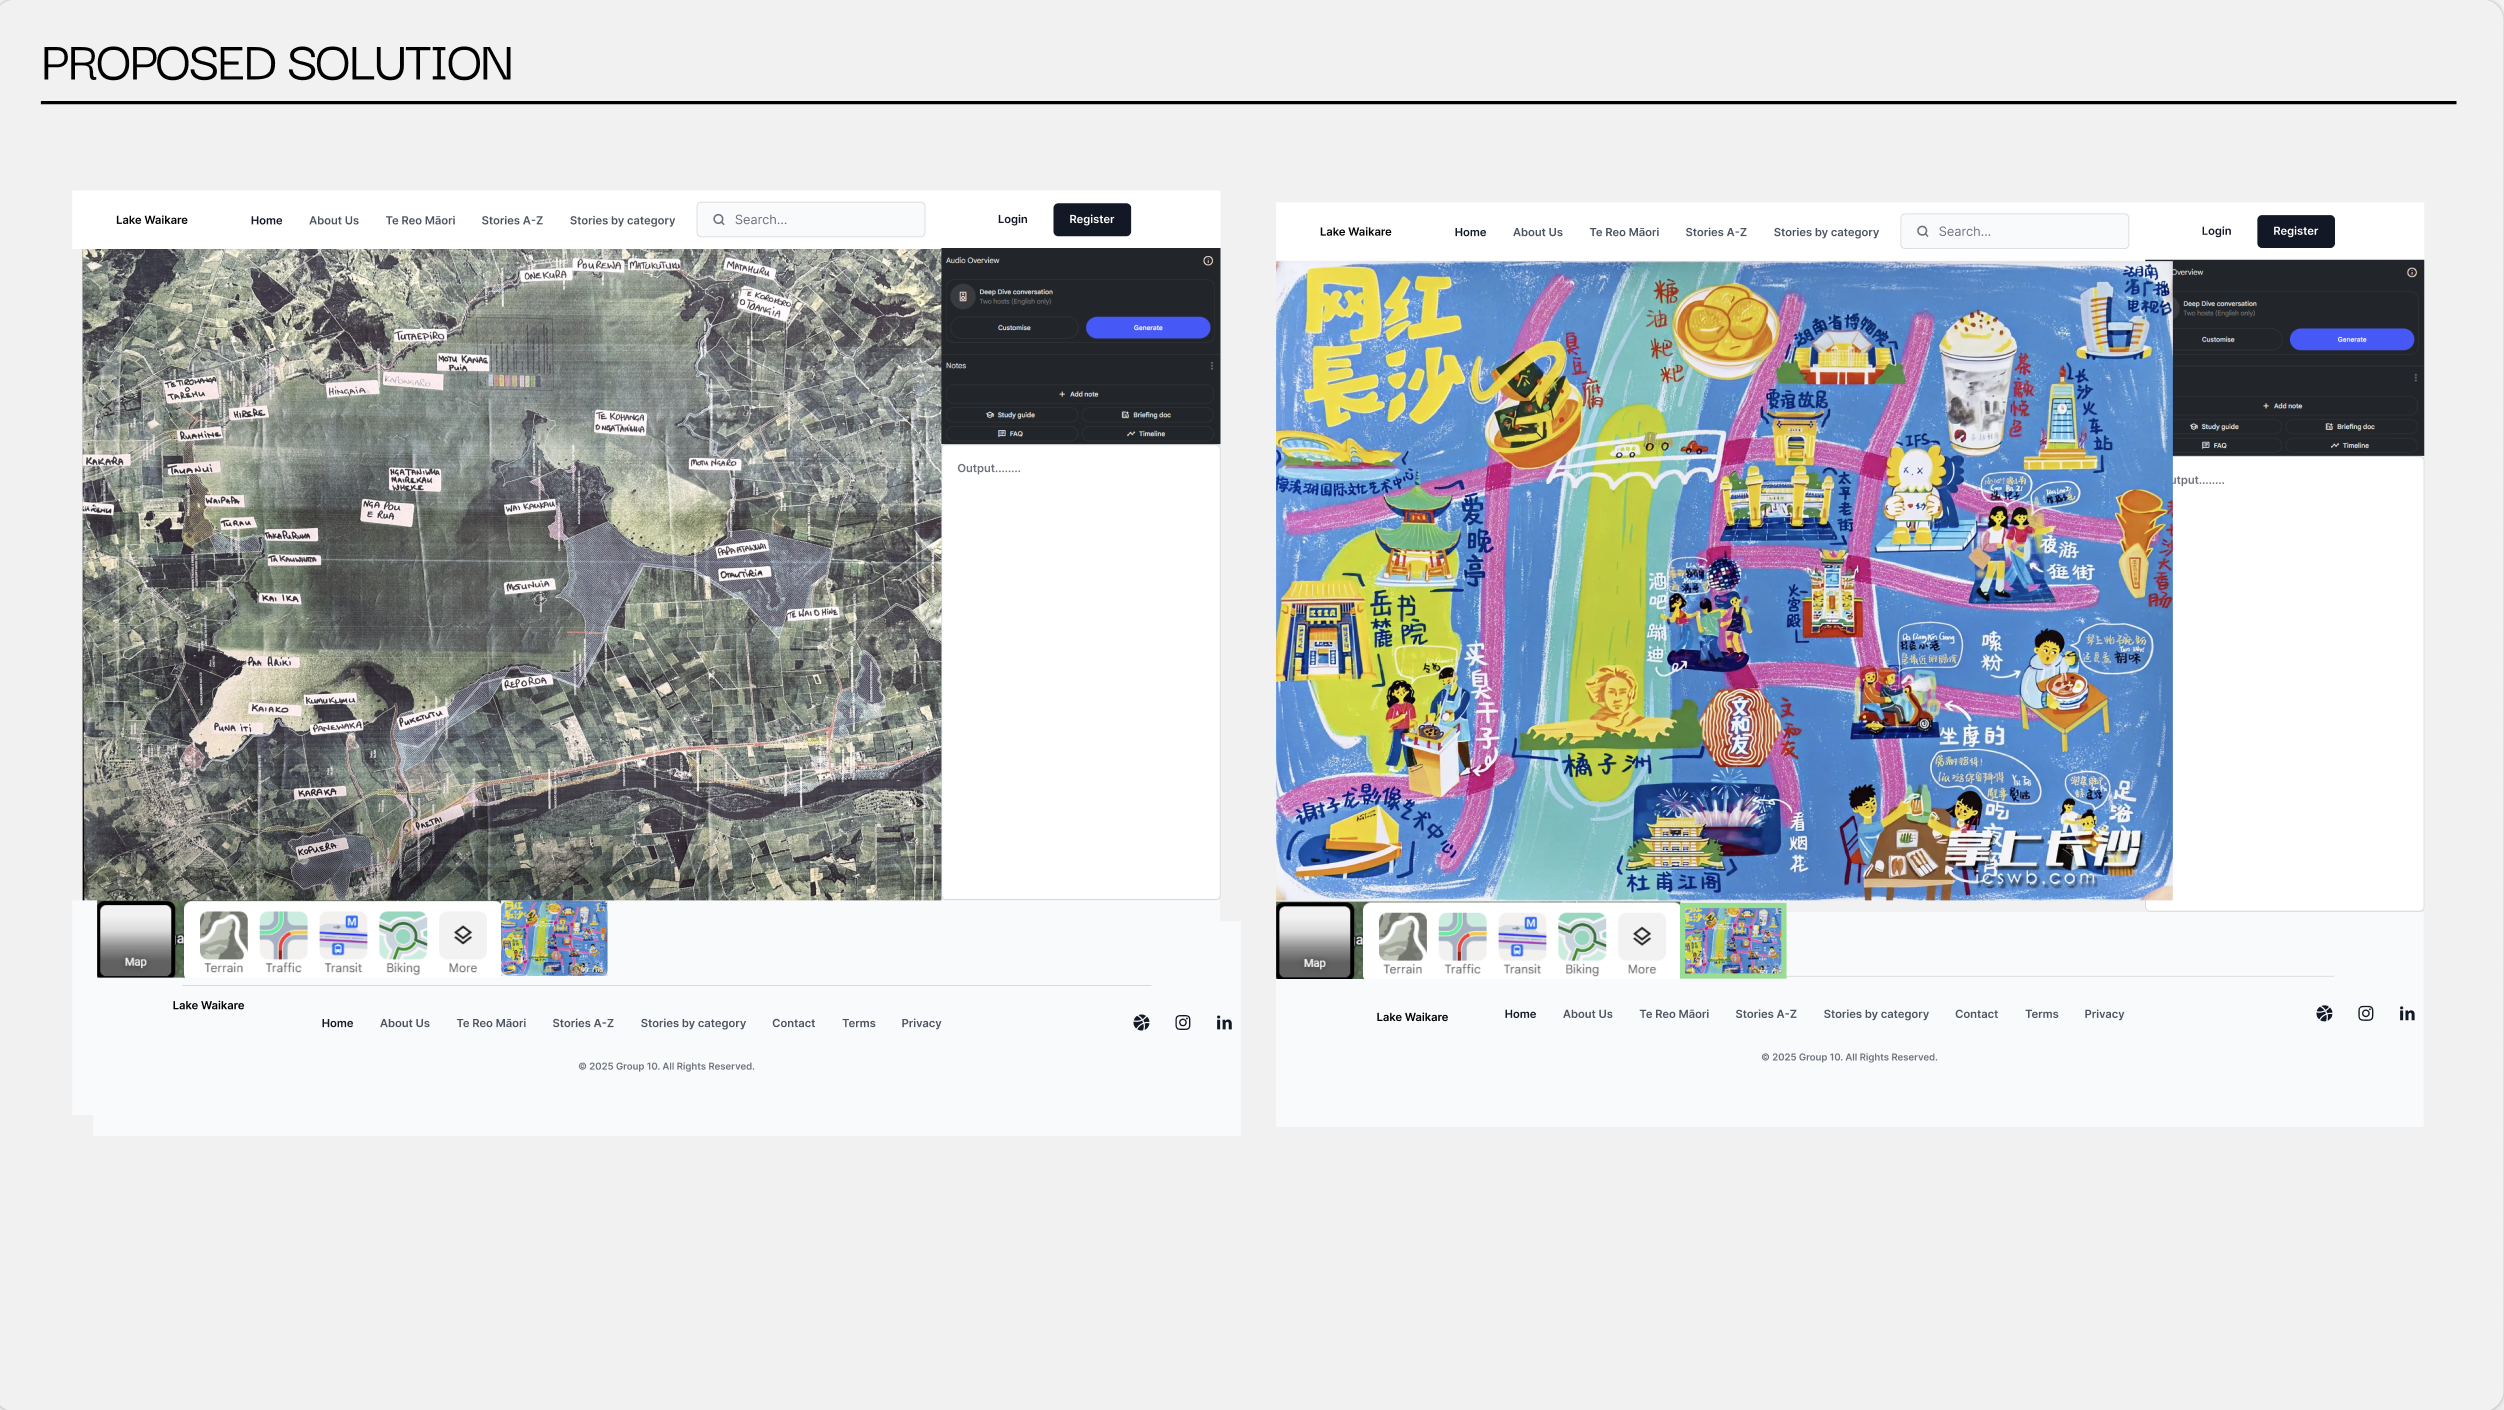
\includegraphics[width=\textwidth]{screenshot/priliminary_design.png}
    \caption{Design}
  \end{subfigure}\hfill
  \begin{subfigure}[b]{0.3\textwidth}
    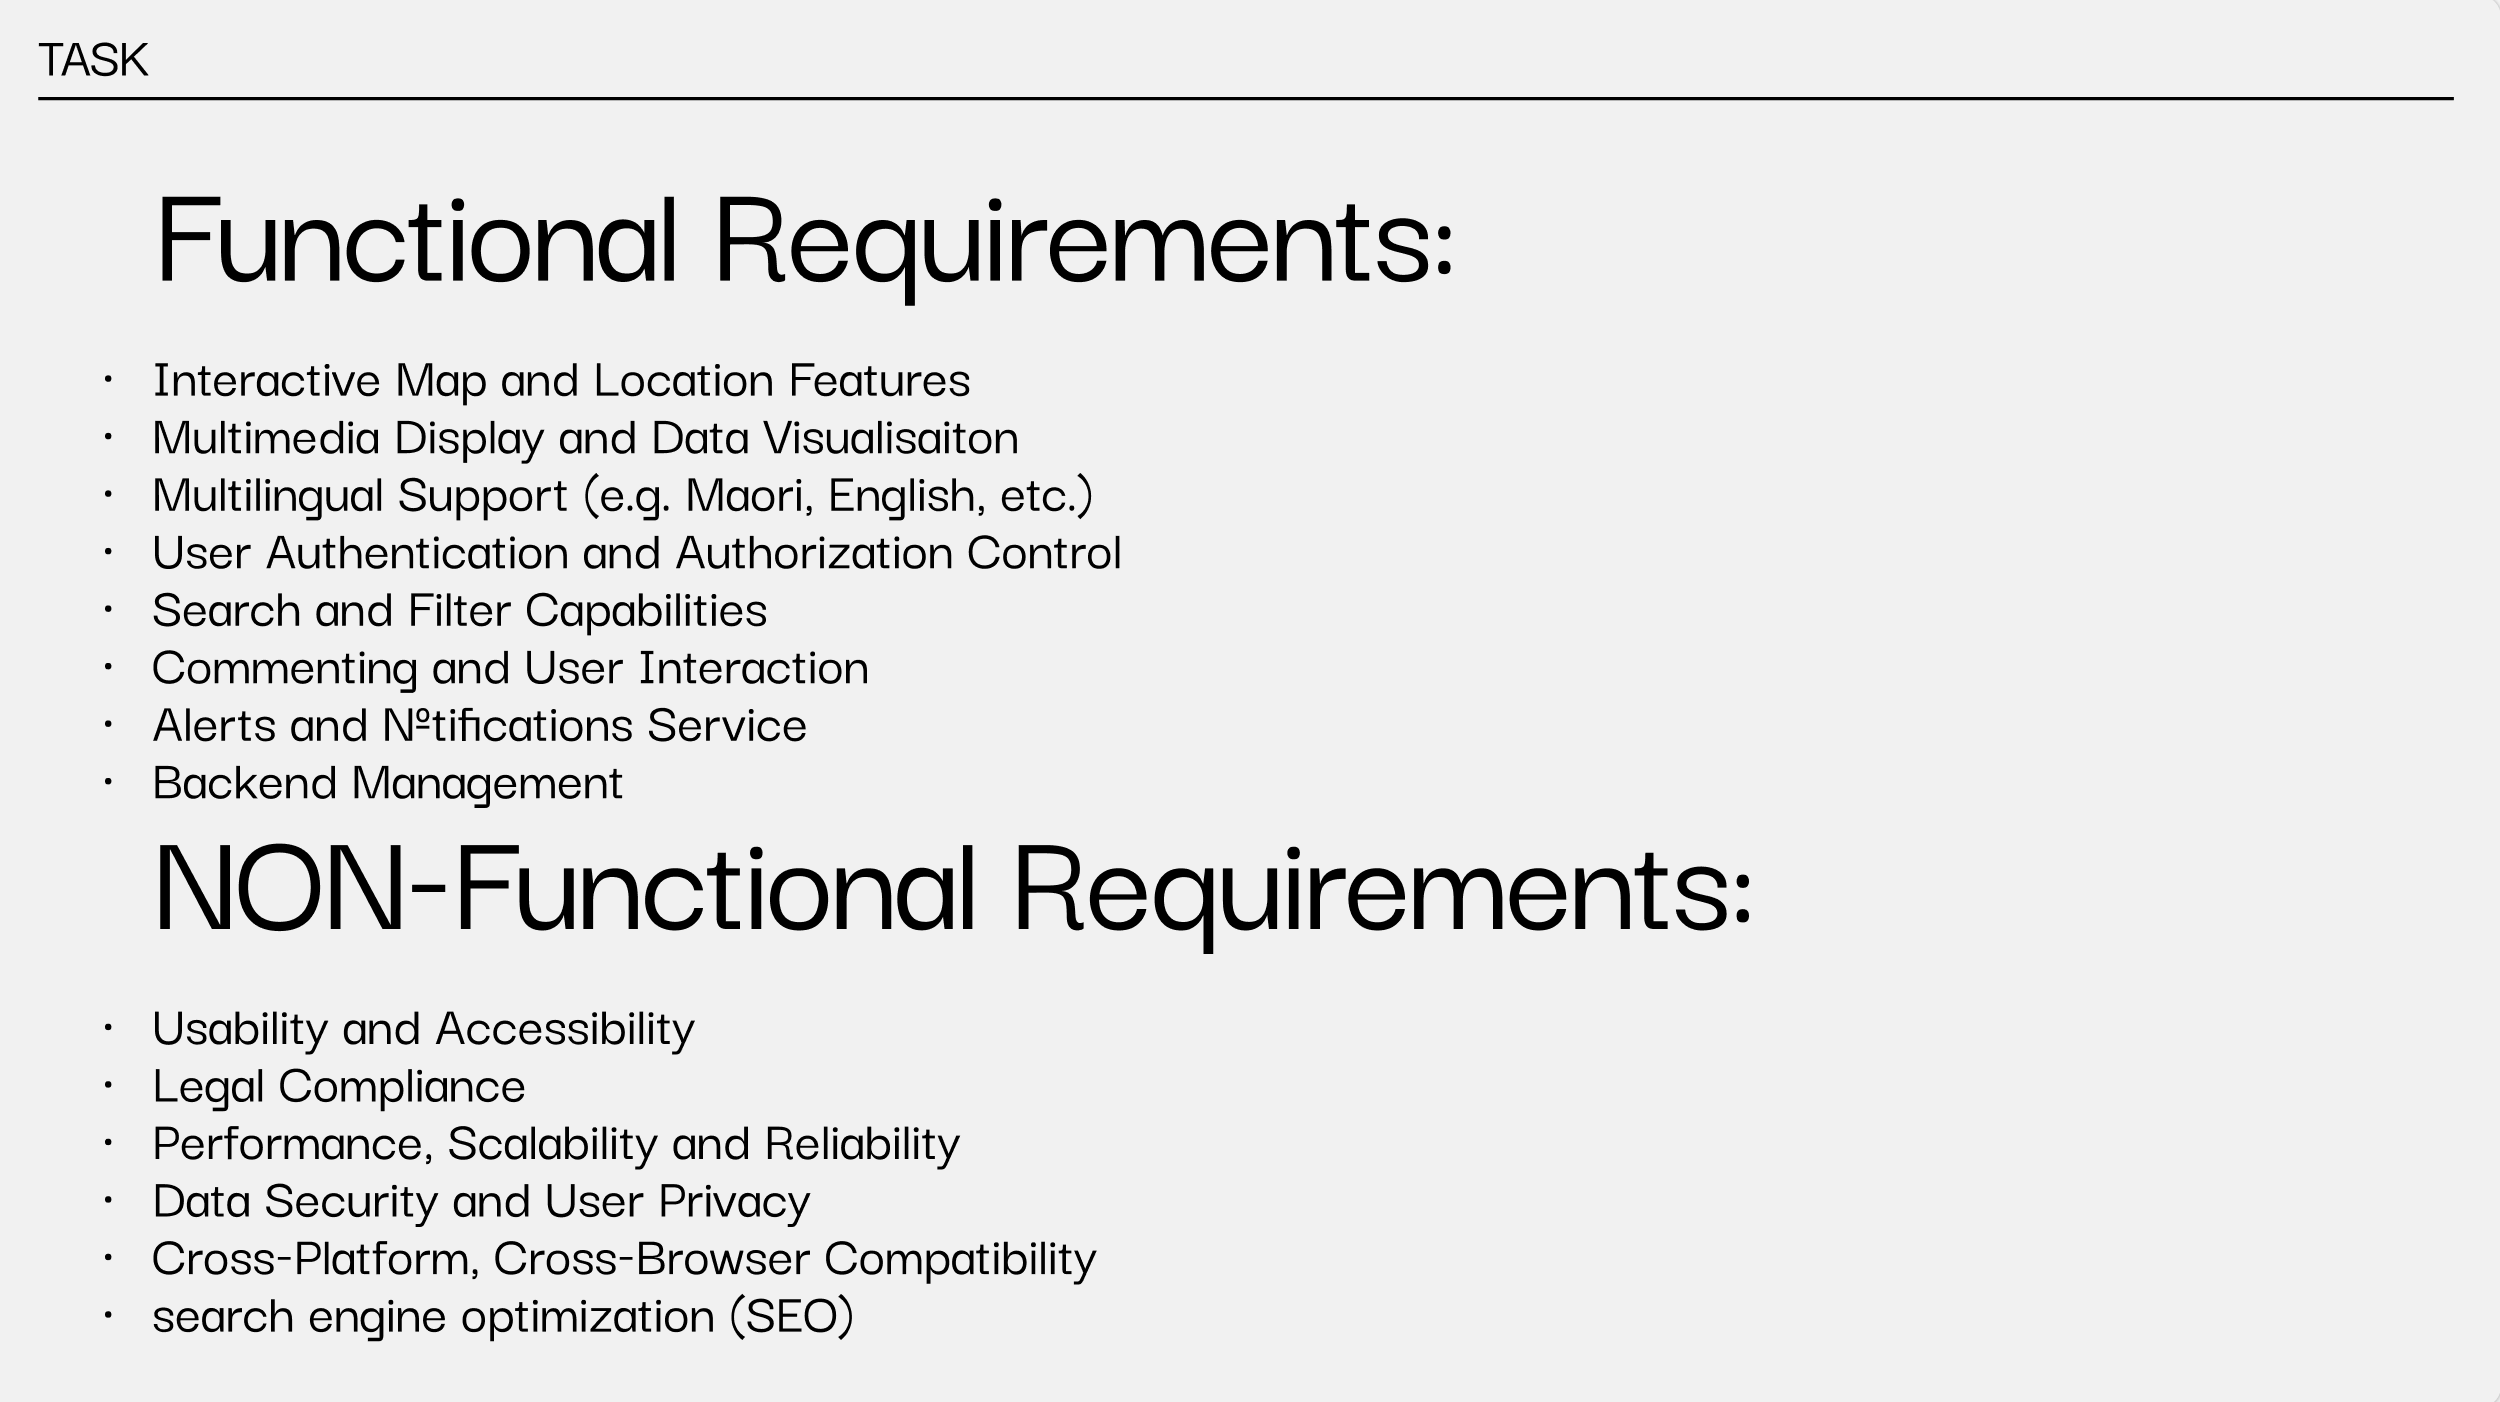
\includegraphics[width=\textwidth]{screenshot/priliminary_feature.png}
    \caption{Feature}
  \end{subfigure}\hfill
  \begin{subfigure}[b]{0.3\textwidth}
    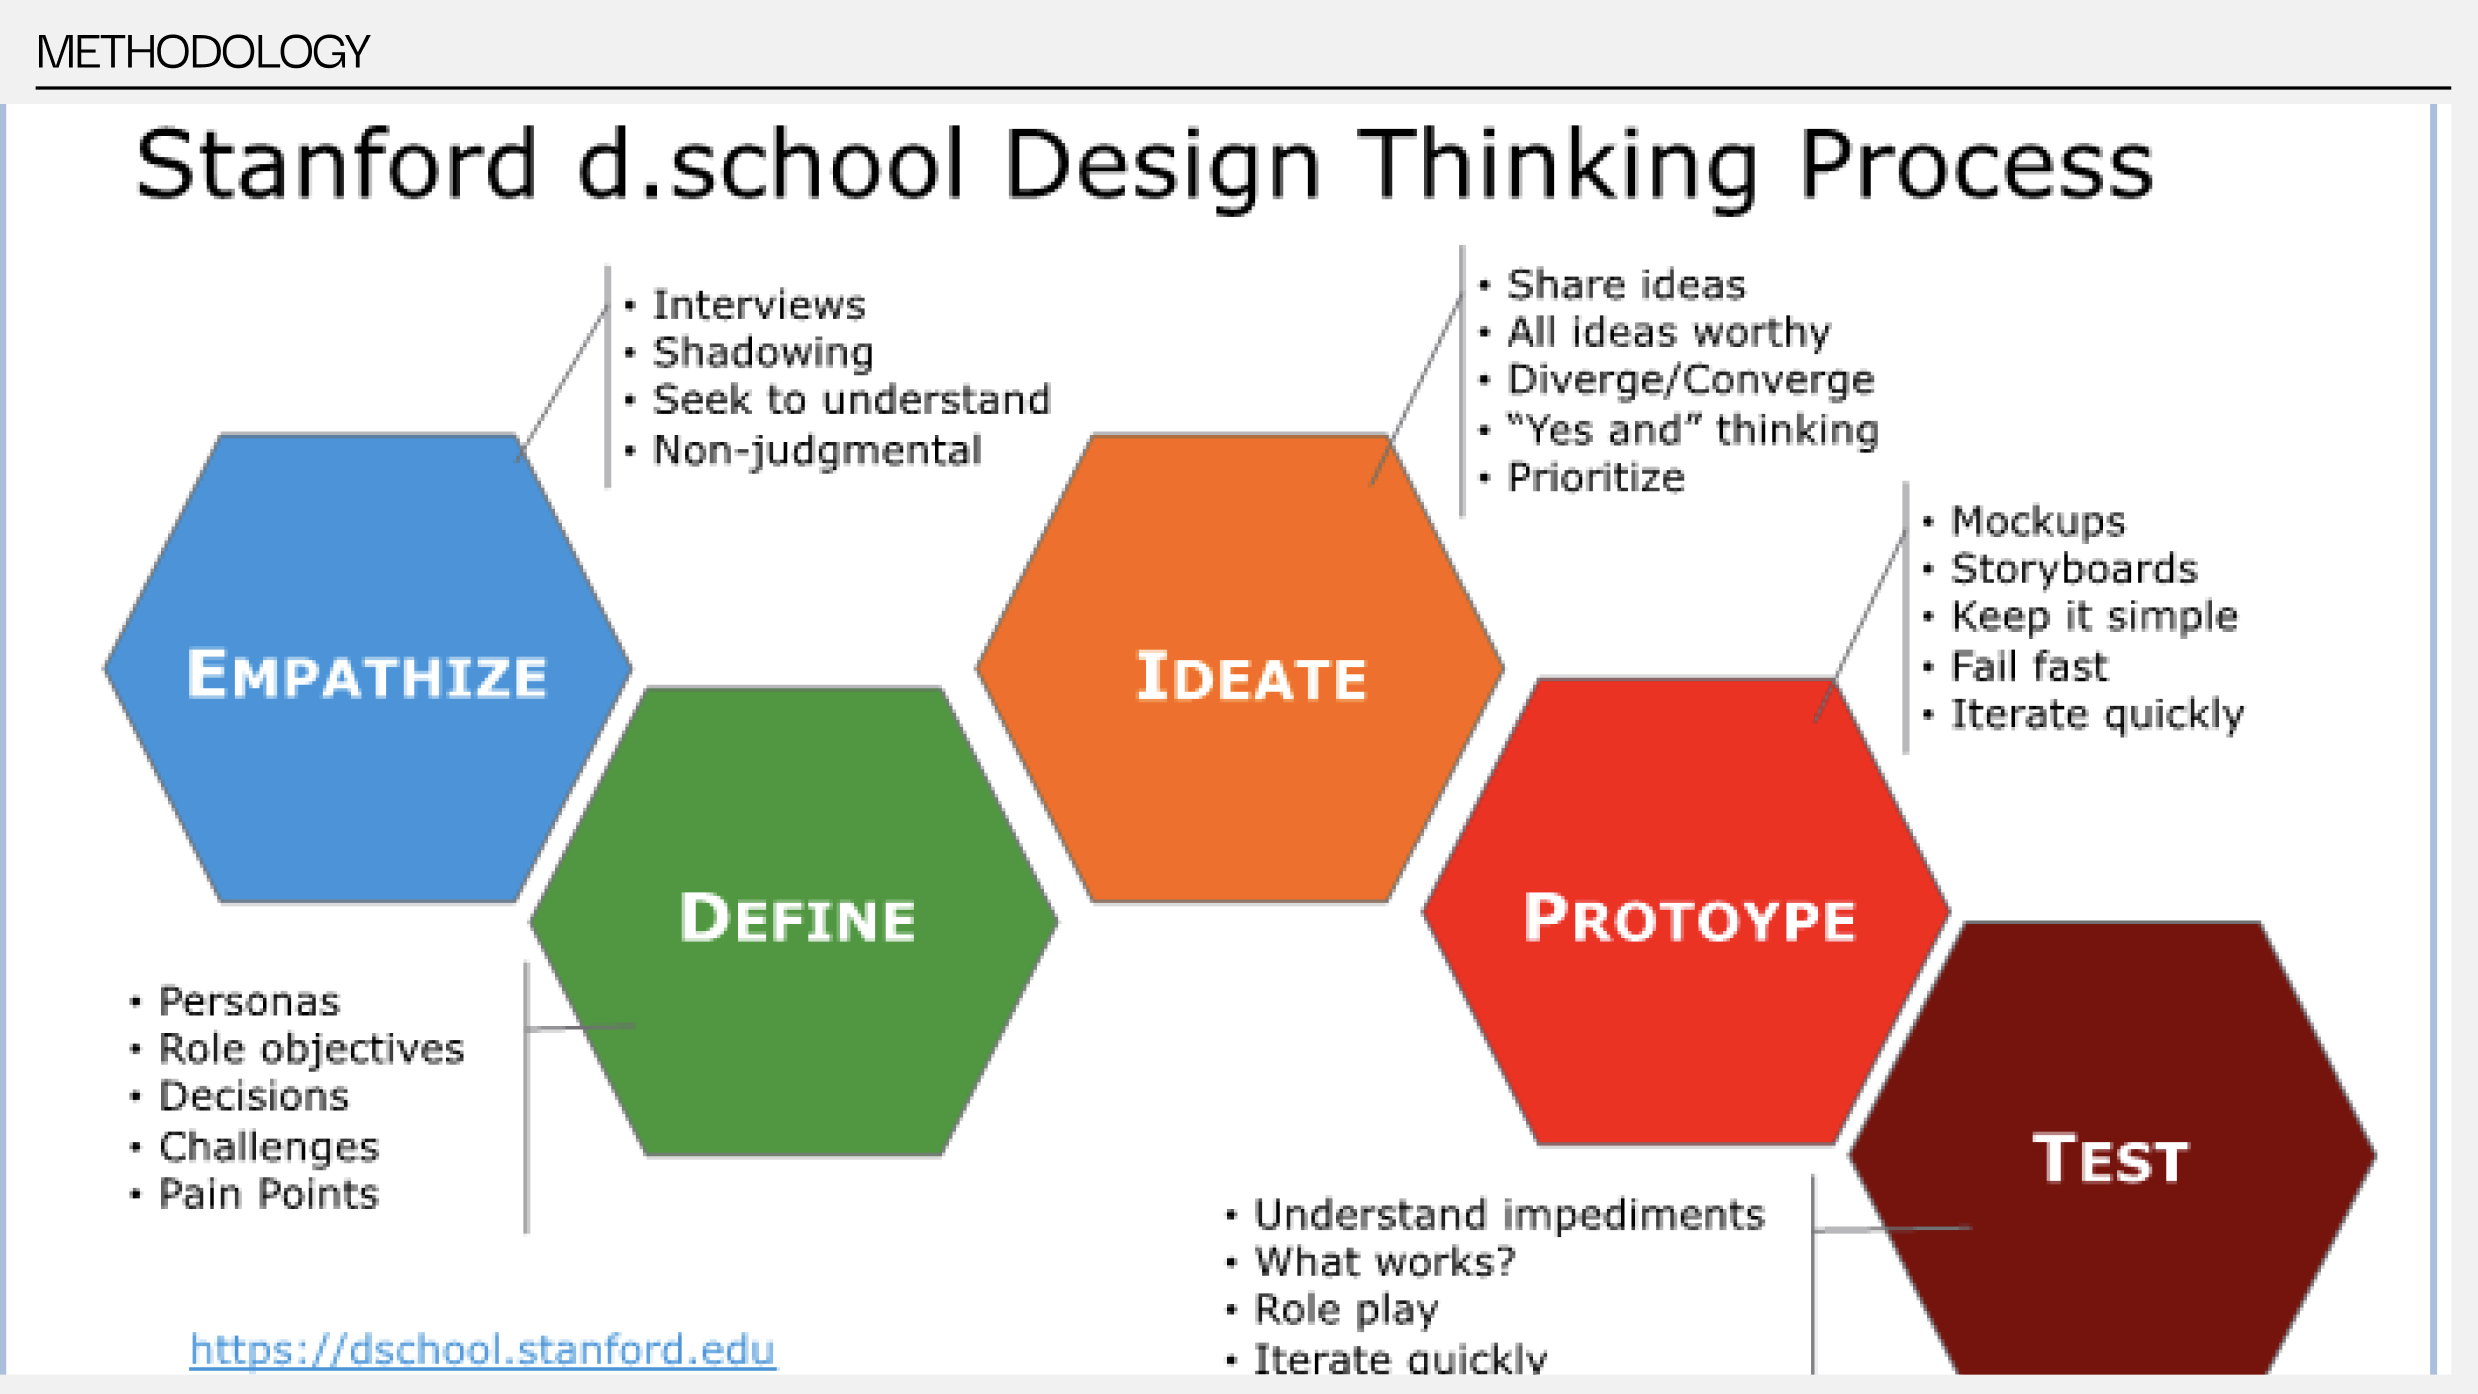
\includegraphics[width=\textwidth]{screenshot/priliminary_methods.png}
    \caption{Methods}
  \end{subfigure}

  \vspace{0.5cm}

  \begin{subfigure}[b]{0.3\textwidth}
    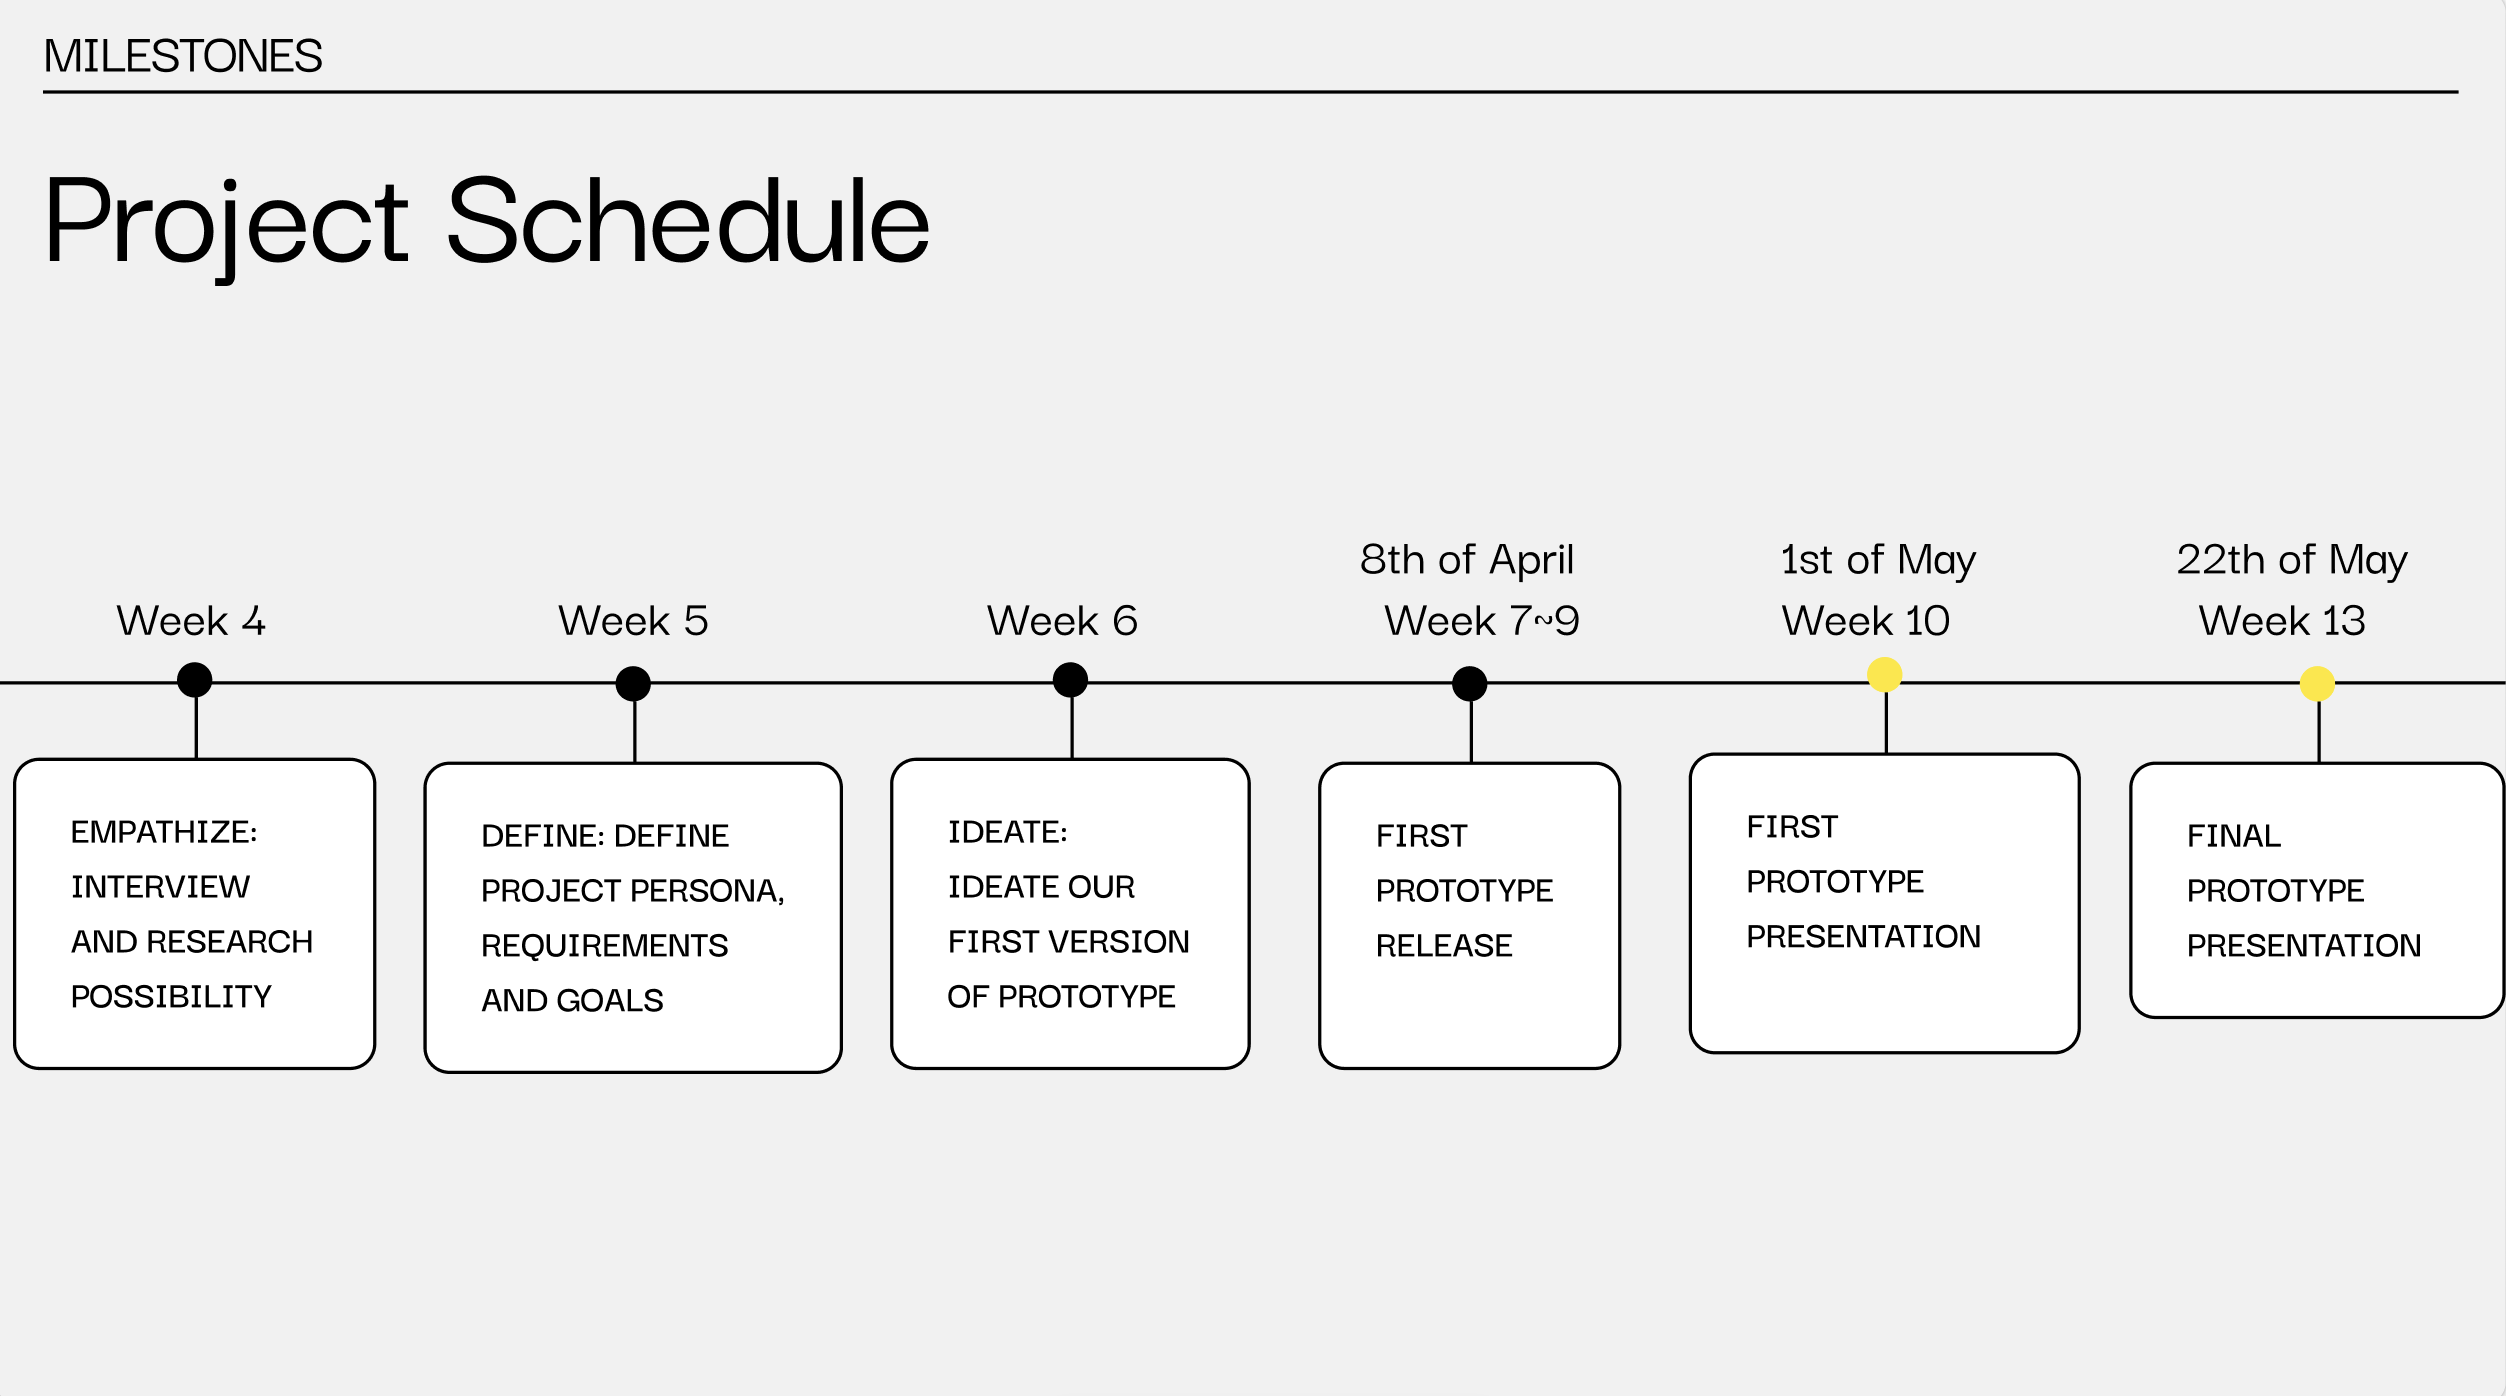
\includegraphics[width=\textwidth]{screenshot/priliminary_milestones.png}
    \caption{Milestones}
  \end{subfigure}
  \caption{Preliminary Design Stage Images}
  \label{fig:preliminary}
\end{figure}

% Wireframe Stage
\subsection{Wireframe Stage}
\begin{figure}[H]
  \centering
  % line 1
  \begin{subfigure}[b]{0.3\textwidth}
    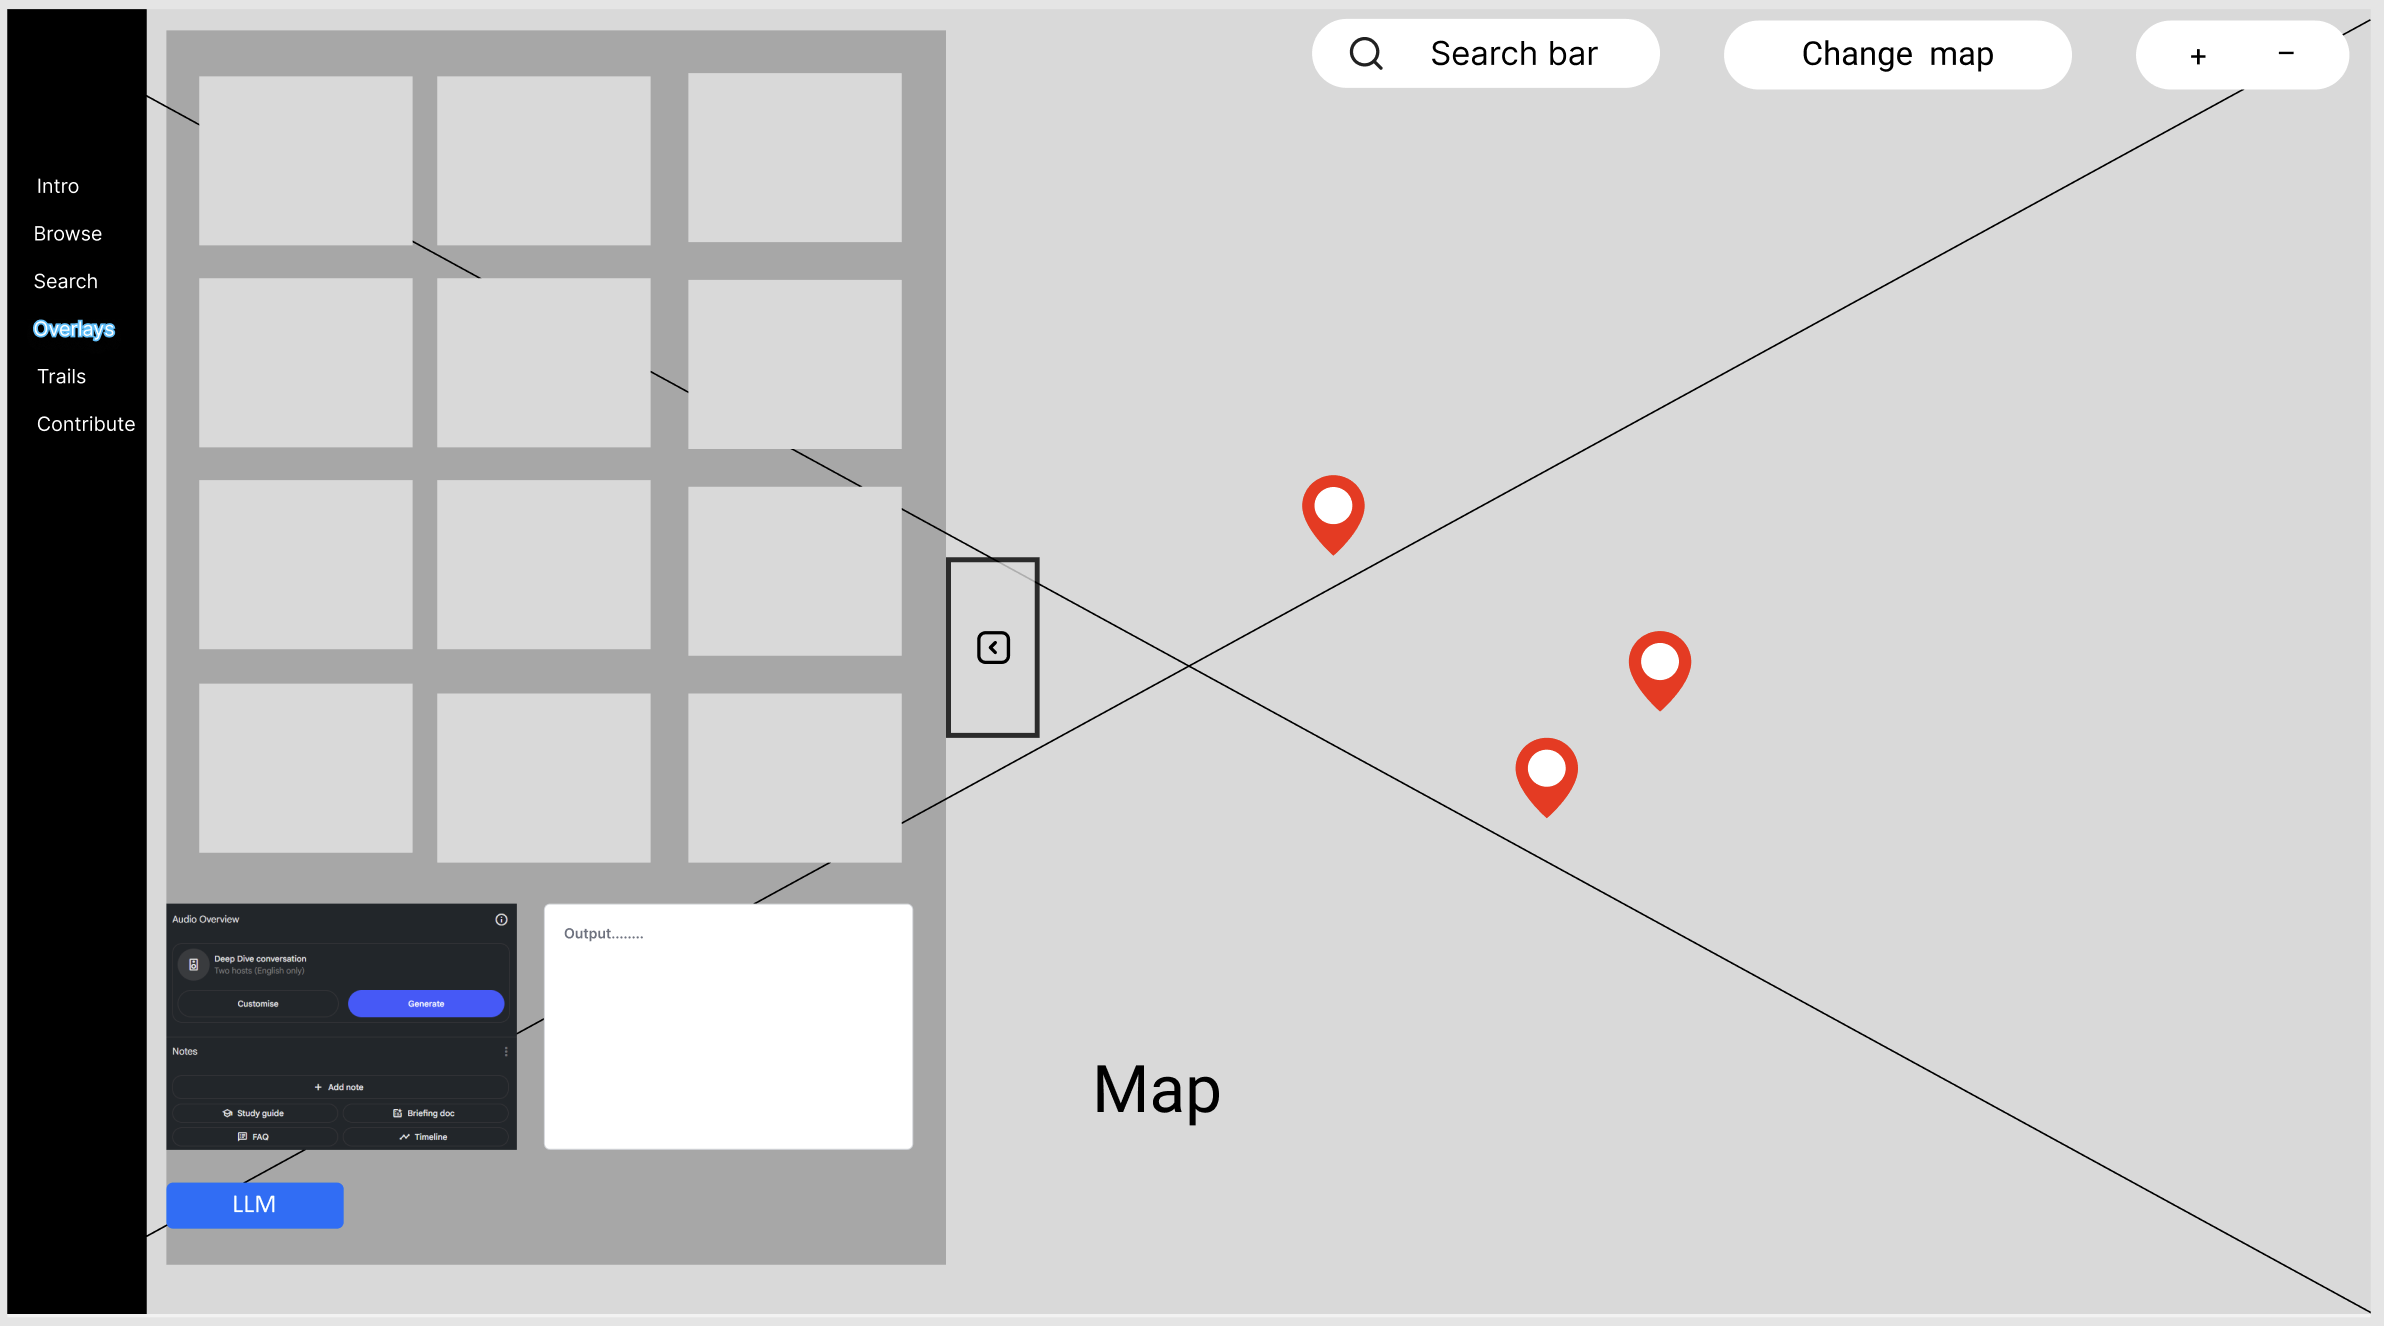
\includegraphics[width=\textwidth]{screenshot/wireframe_llm.png}
    \caption{LLM}
  \end{subfigure}\hfill
  \begin{subfigure}[b]{0.3\textwidth}
    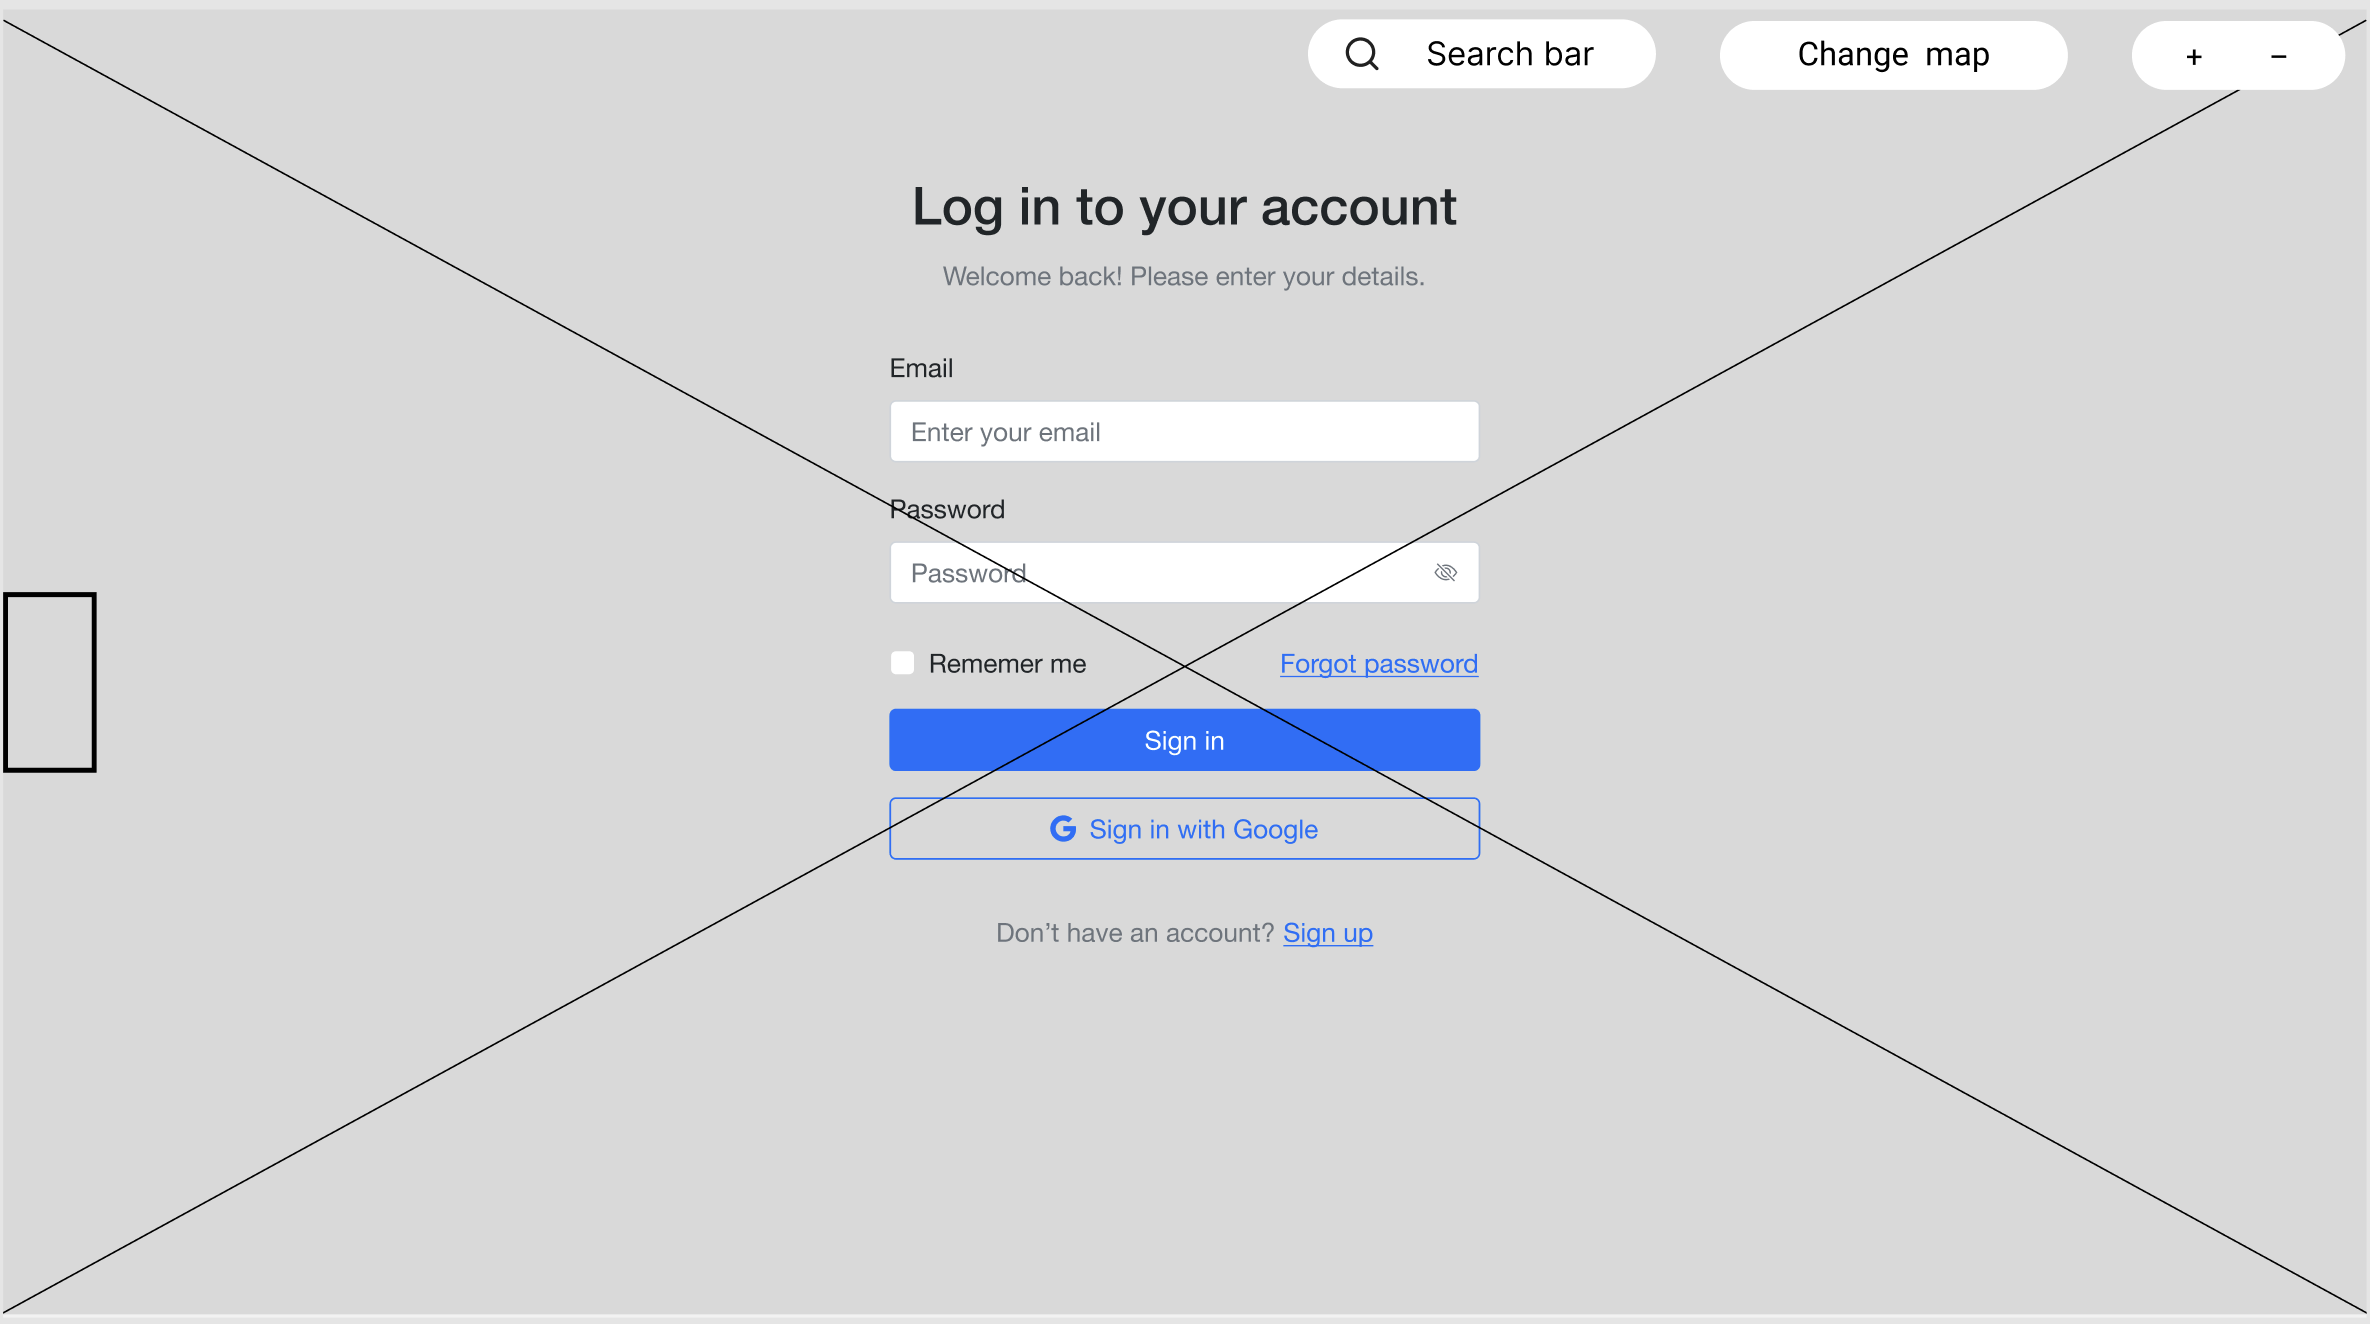
\includegraphics[width=\textwidth]{screenshot/wireframe_login.png}
    \caption{Login}
  \end{subfigure}\hfill
  \begin{subfigure}[b]{0.3\textwidth}
    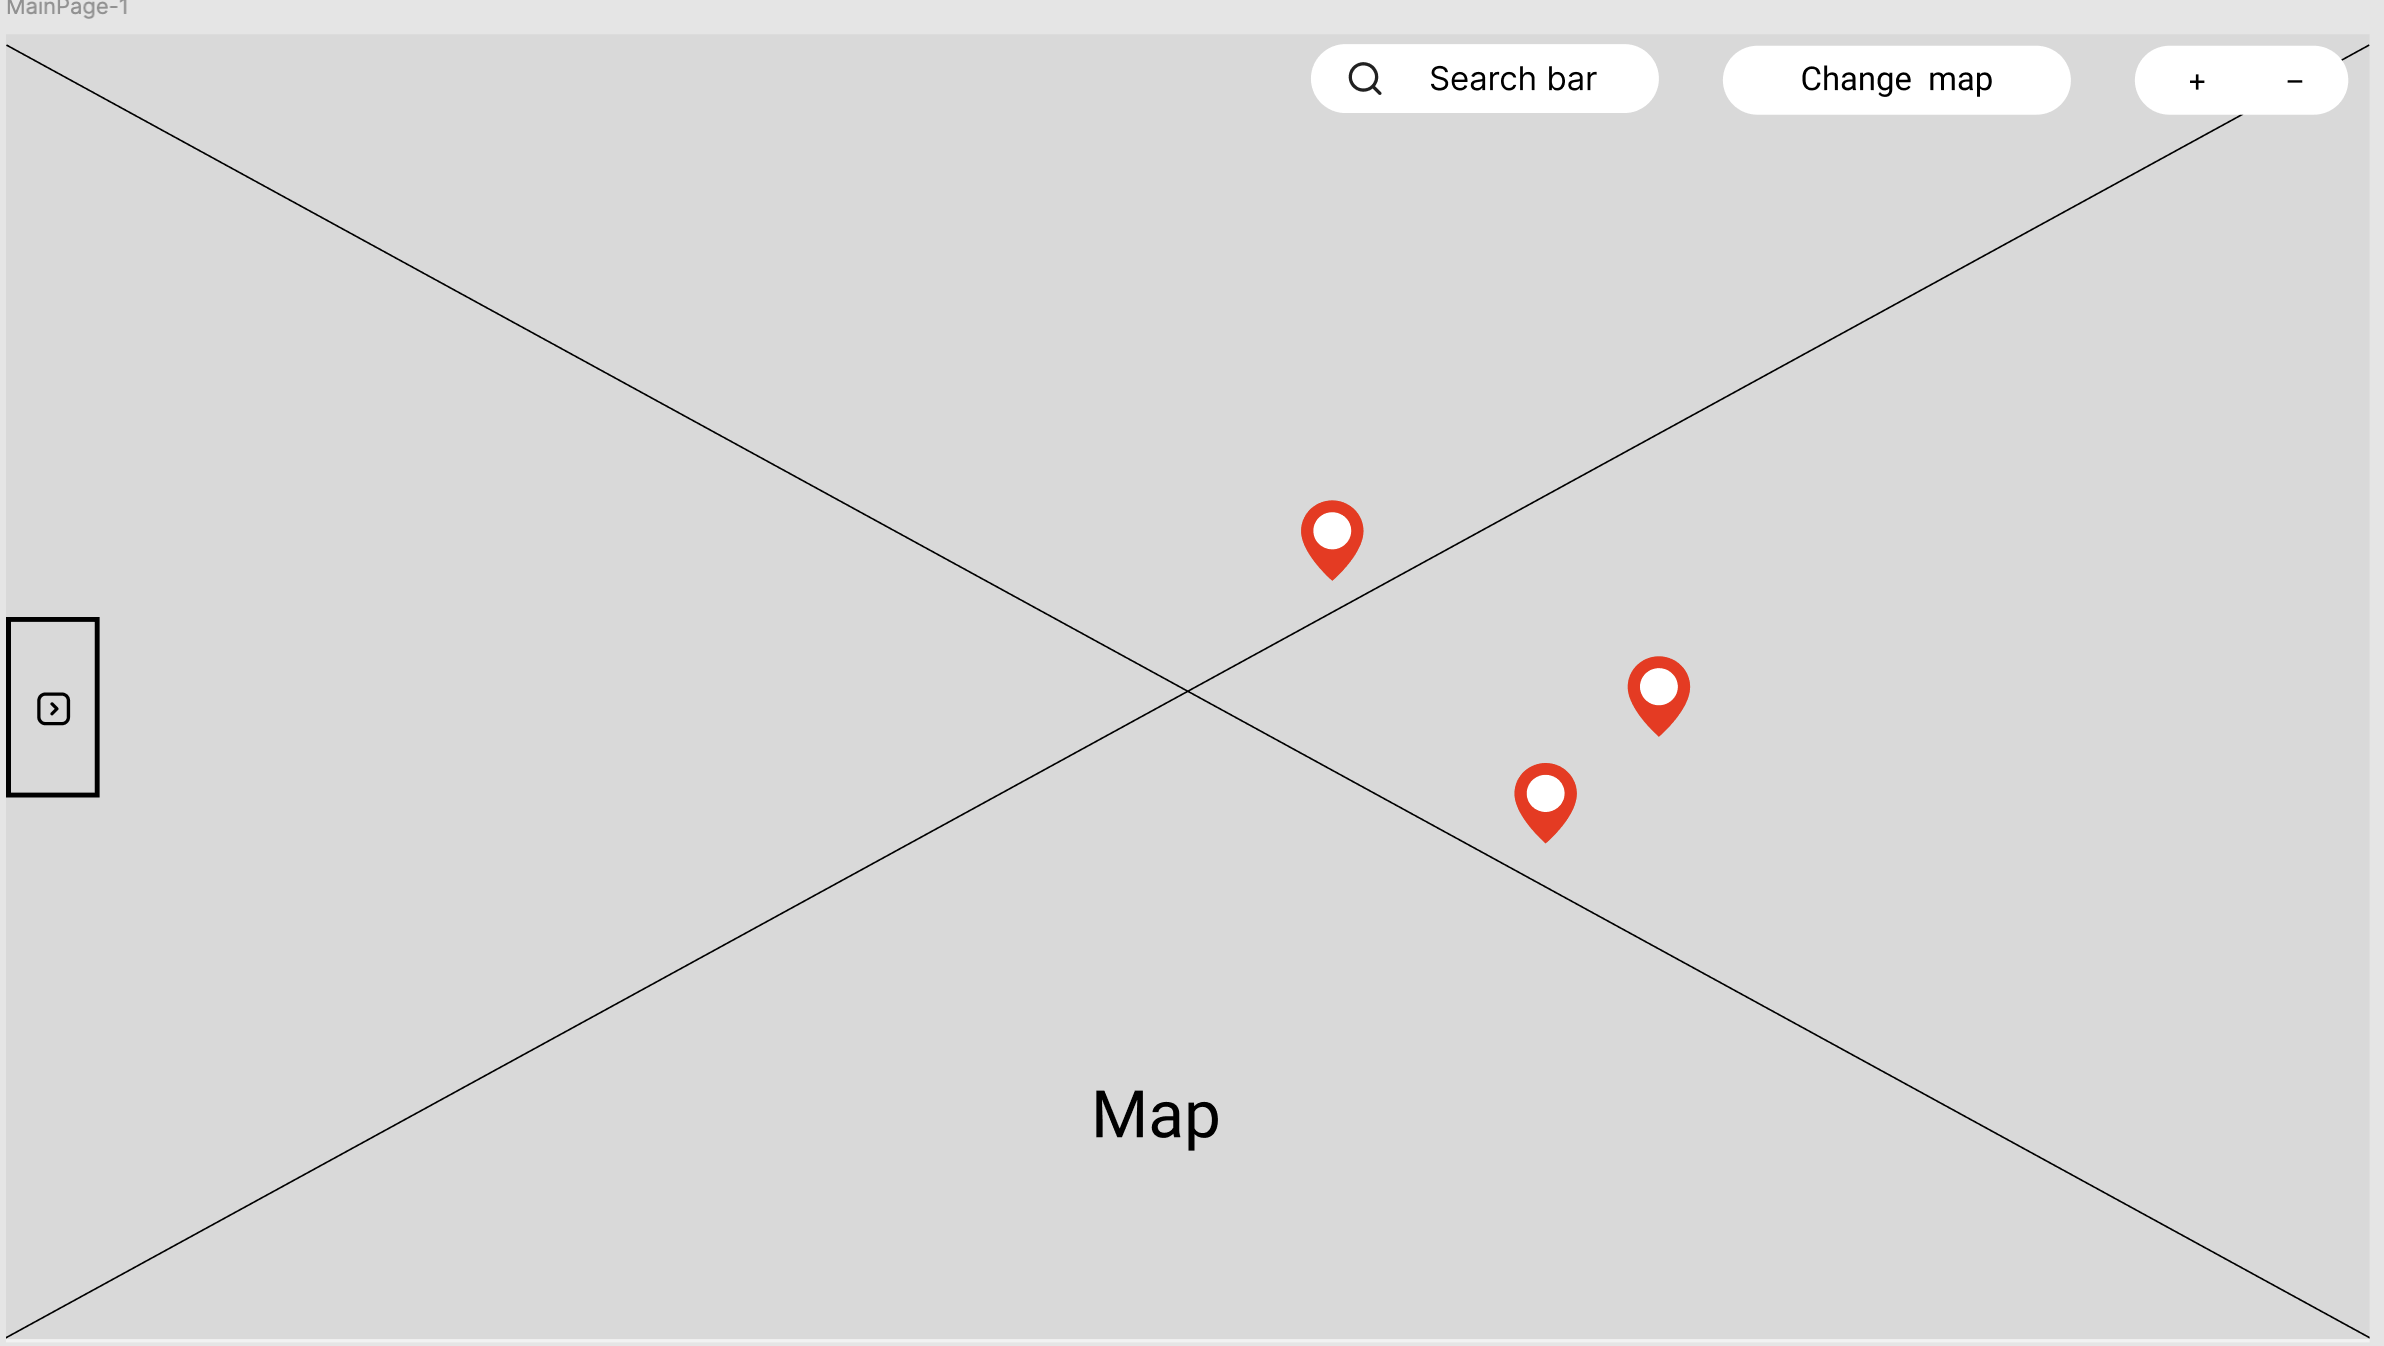
\includegraphics[width=\textwidth]{screenshot/wireframe_main.png}
    \caption{Main}
  \end{subfigure}

  \vspace{0.5cm}

  % line 2
  \begin{subfigure}[b]{0.3\textwidth}
    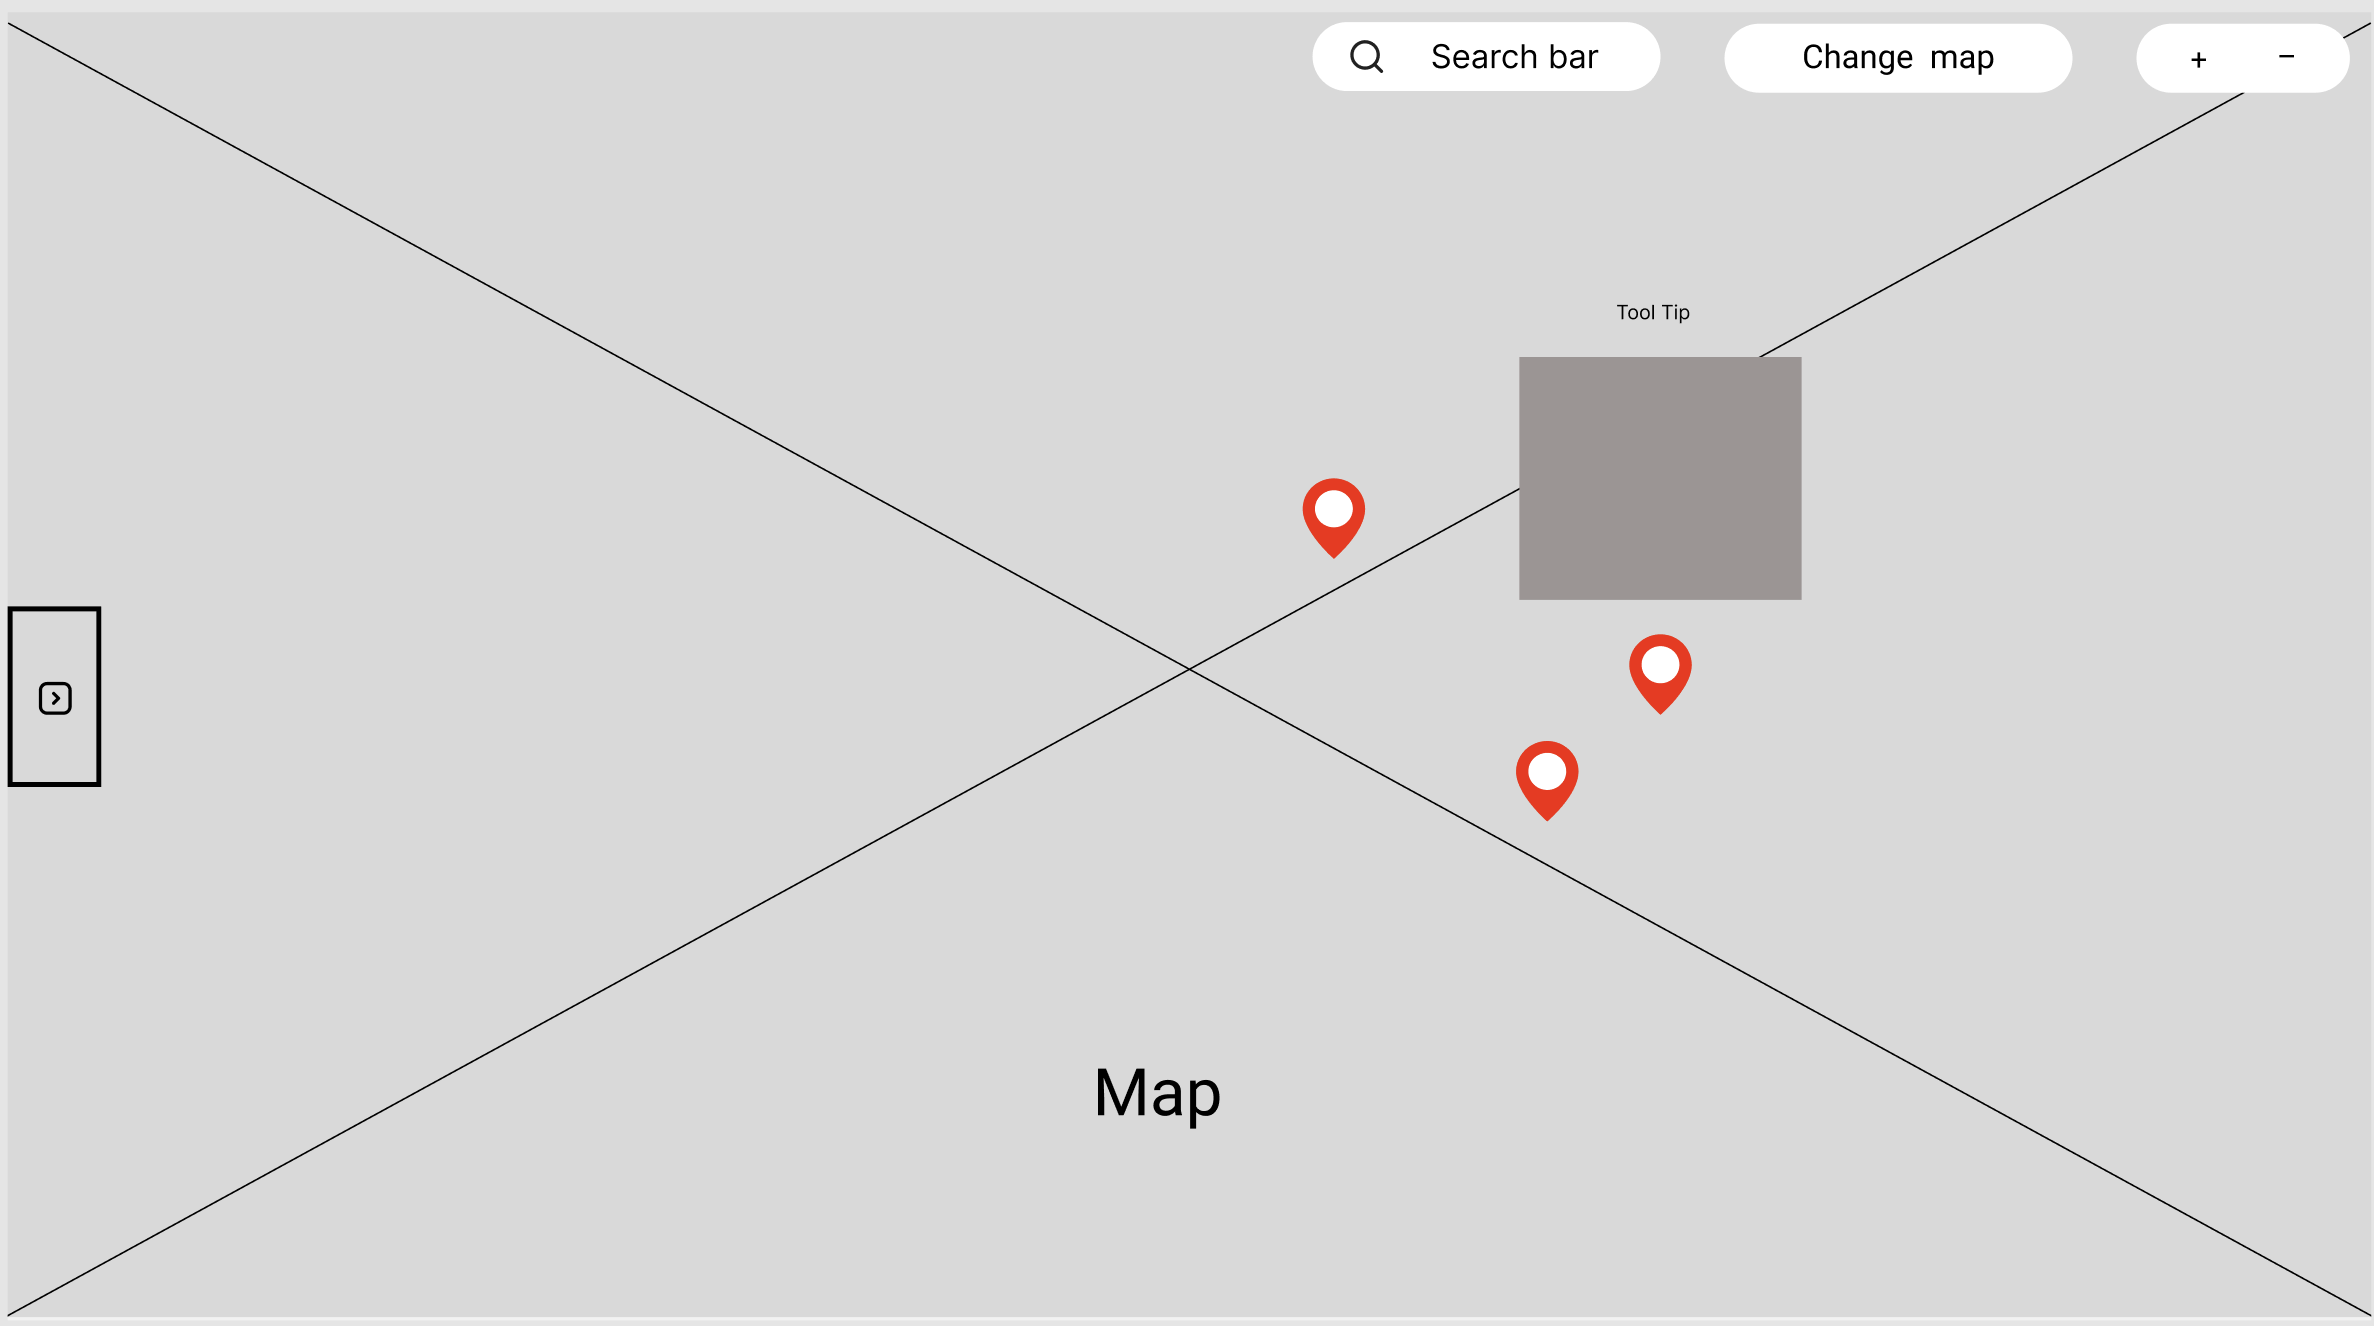
\includegraphics[width=\textwidth]{screenshot/wireframe_map_interaction.png}
    \caption{Map Interaction}
  \end{subfigure}\hfill
  \begin{subfigure}[b]{0.3\textwidth}
    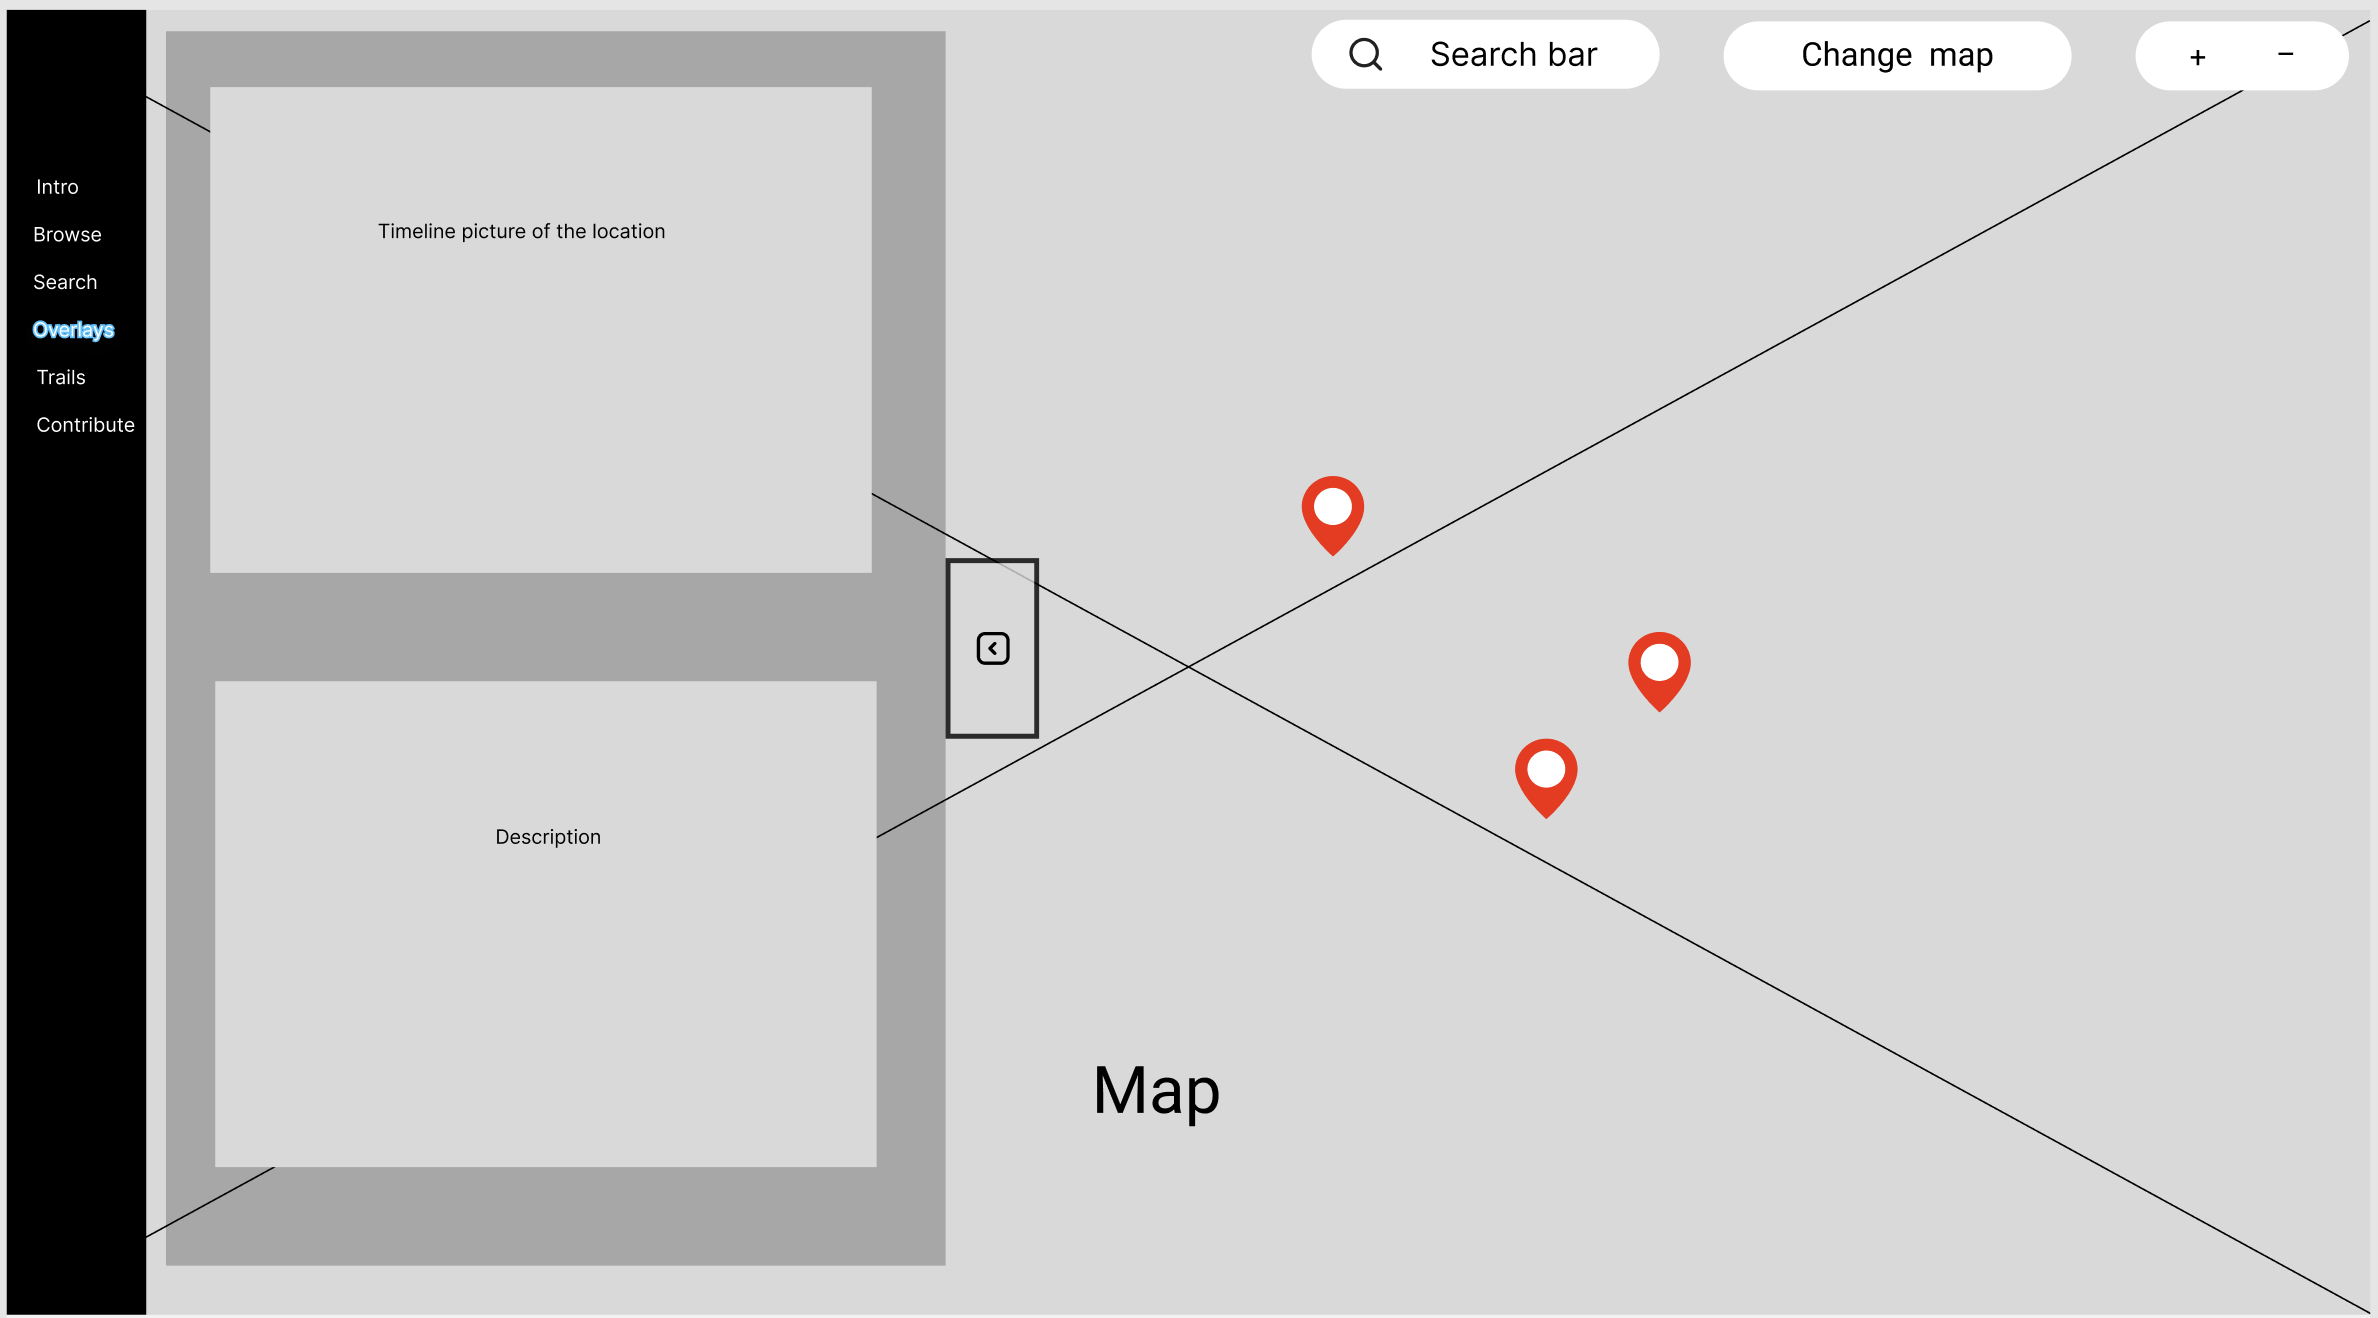
\includegraphics[width=\textwidth]{screenshot/wireframe_overlay2.png}
    \caption{Overlay 2}
  \end{subfigure}\hfill
  \begin{subfigure}[b]{0.3\textwidth}
    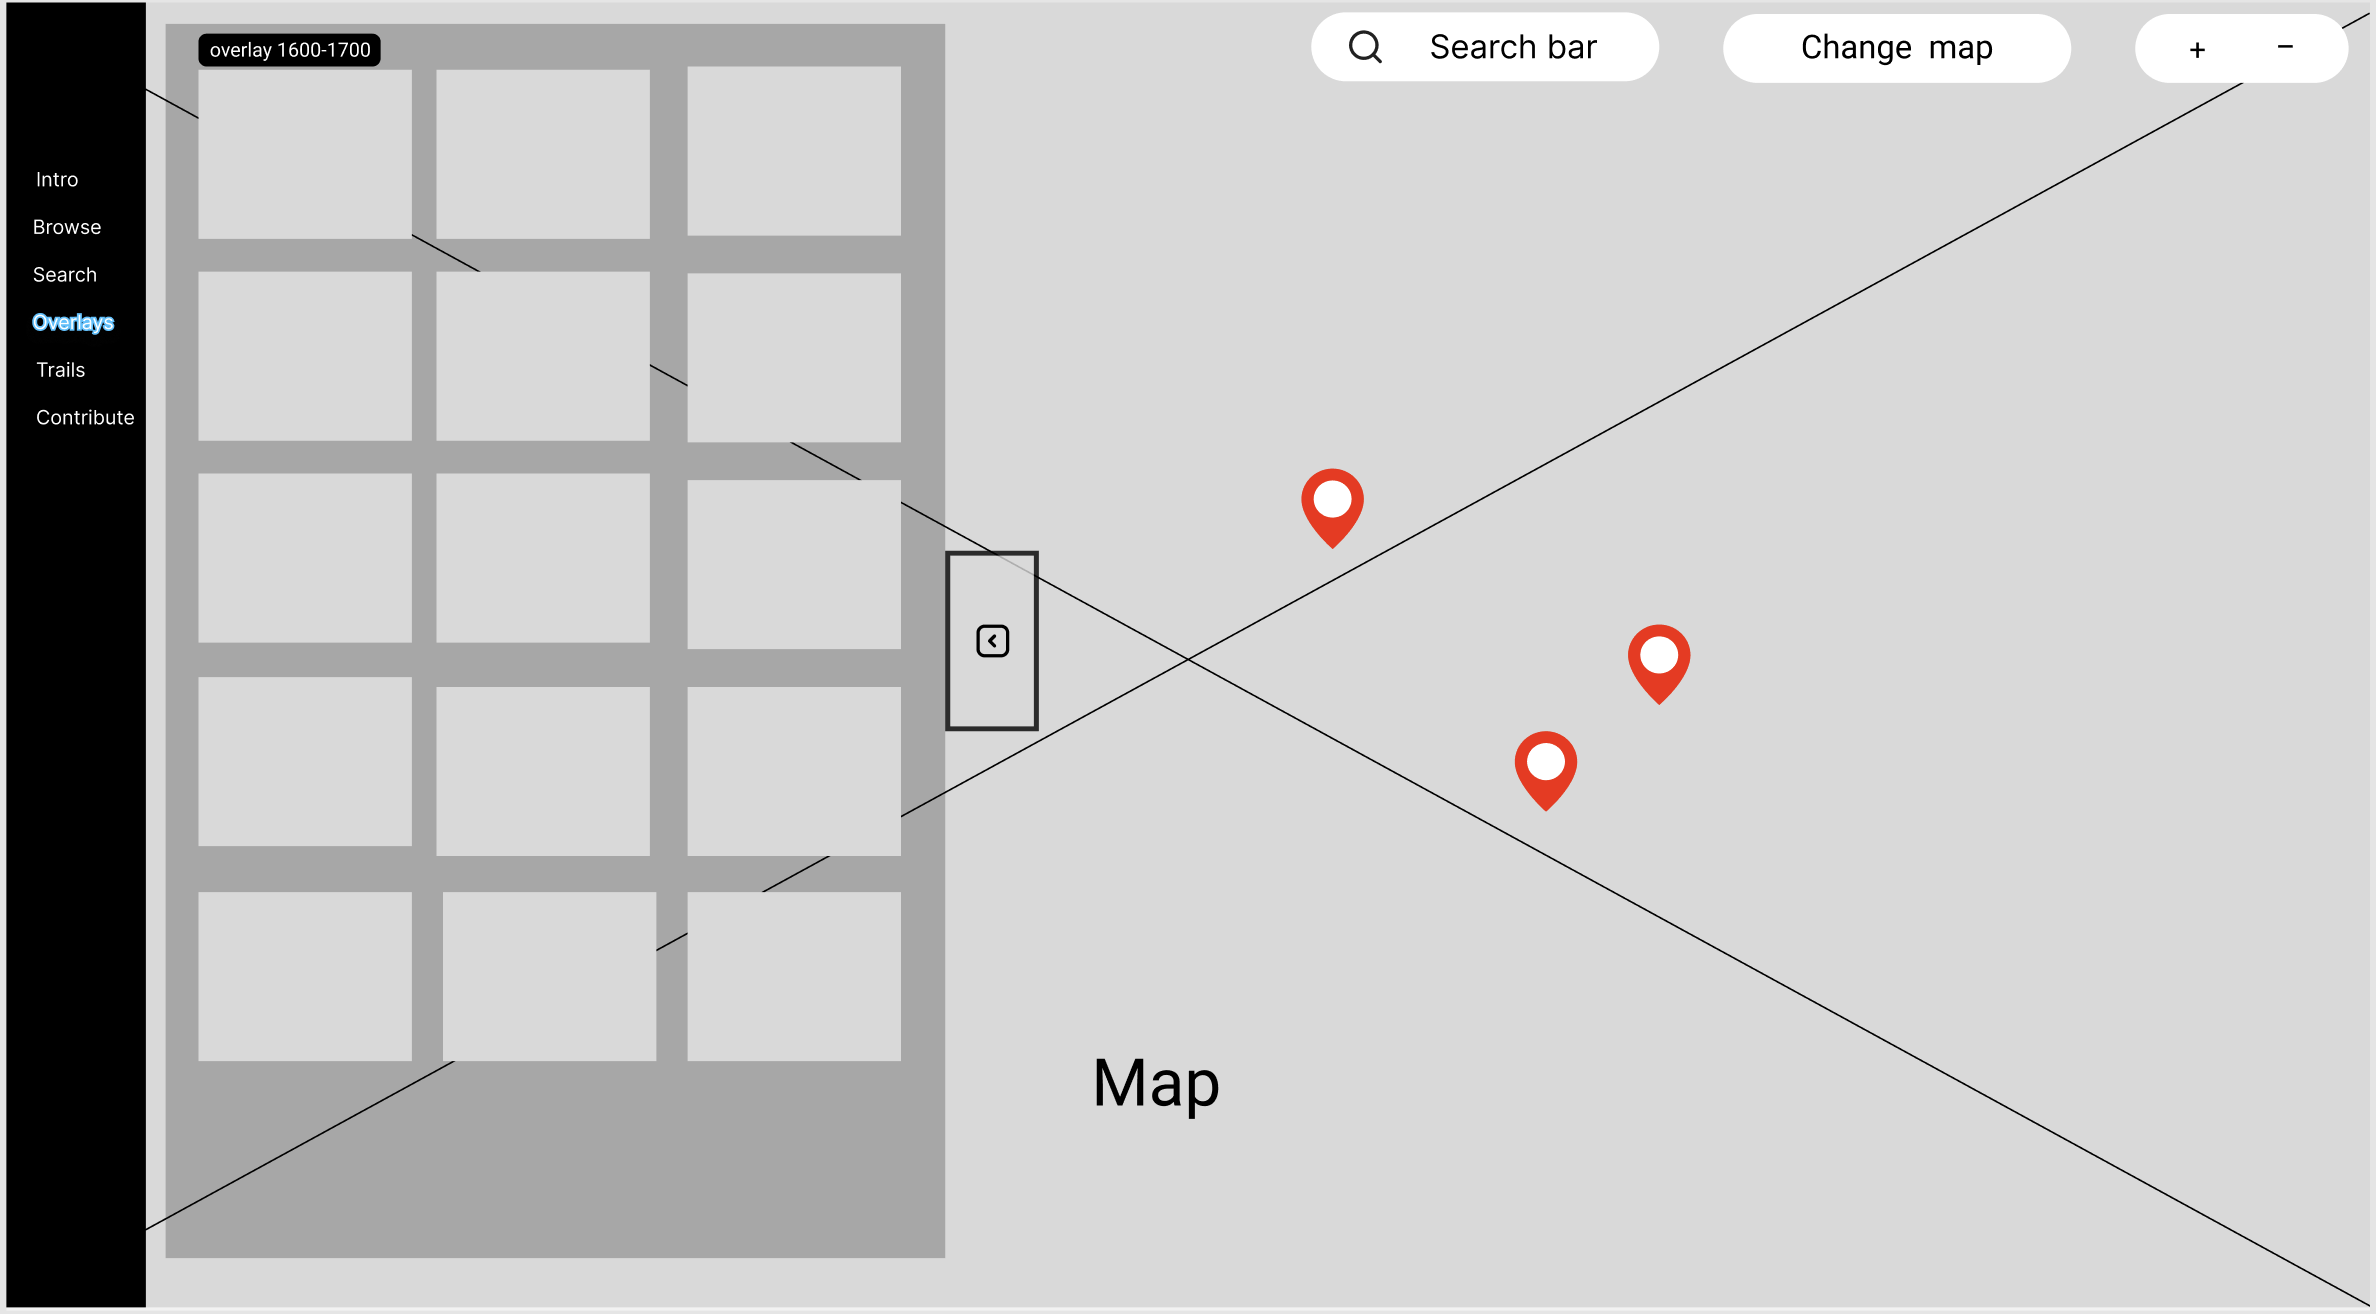
\includegraphics[width=\textwidth]{screenshot/wireframe_overlays.png}
    \caption{Overlays}
  \end{subfigure}

  \vspace{0.5cm}

  % line 3
  \begin{subfigure}[b]{0.3\textwidth}
    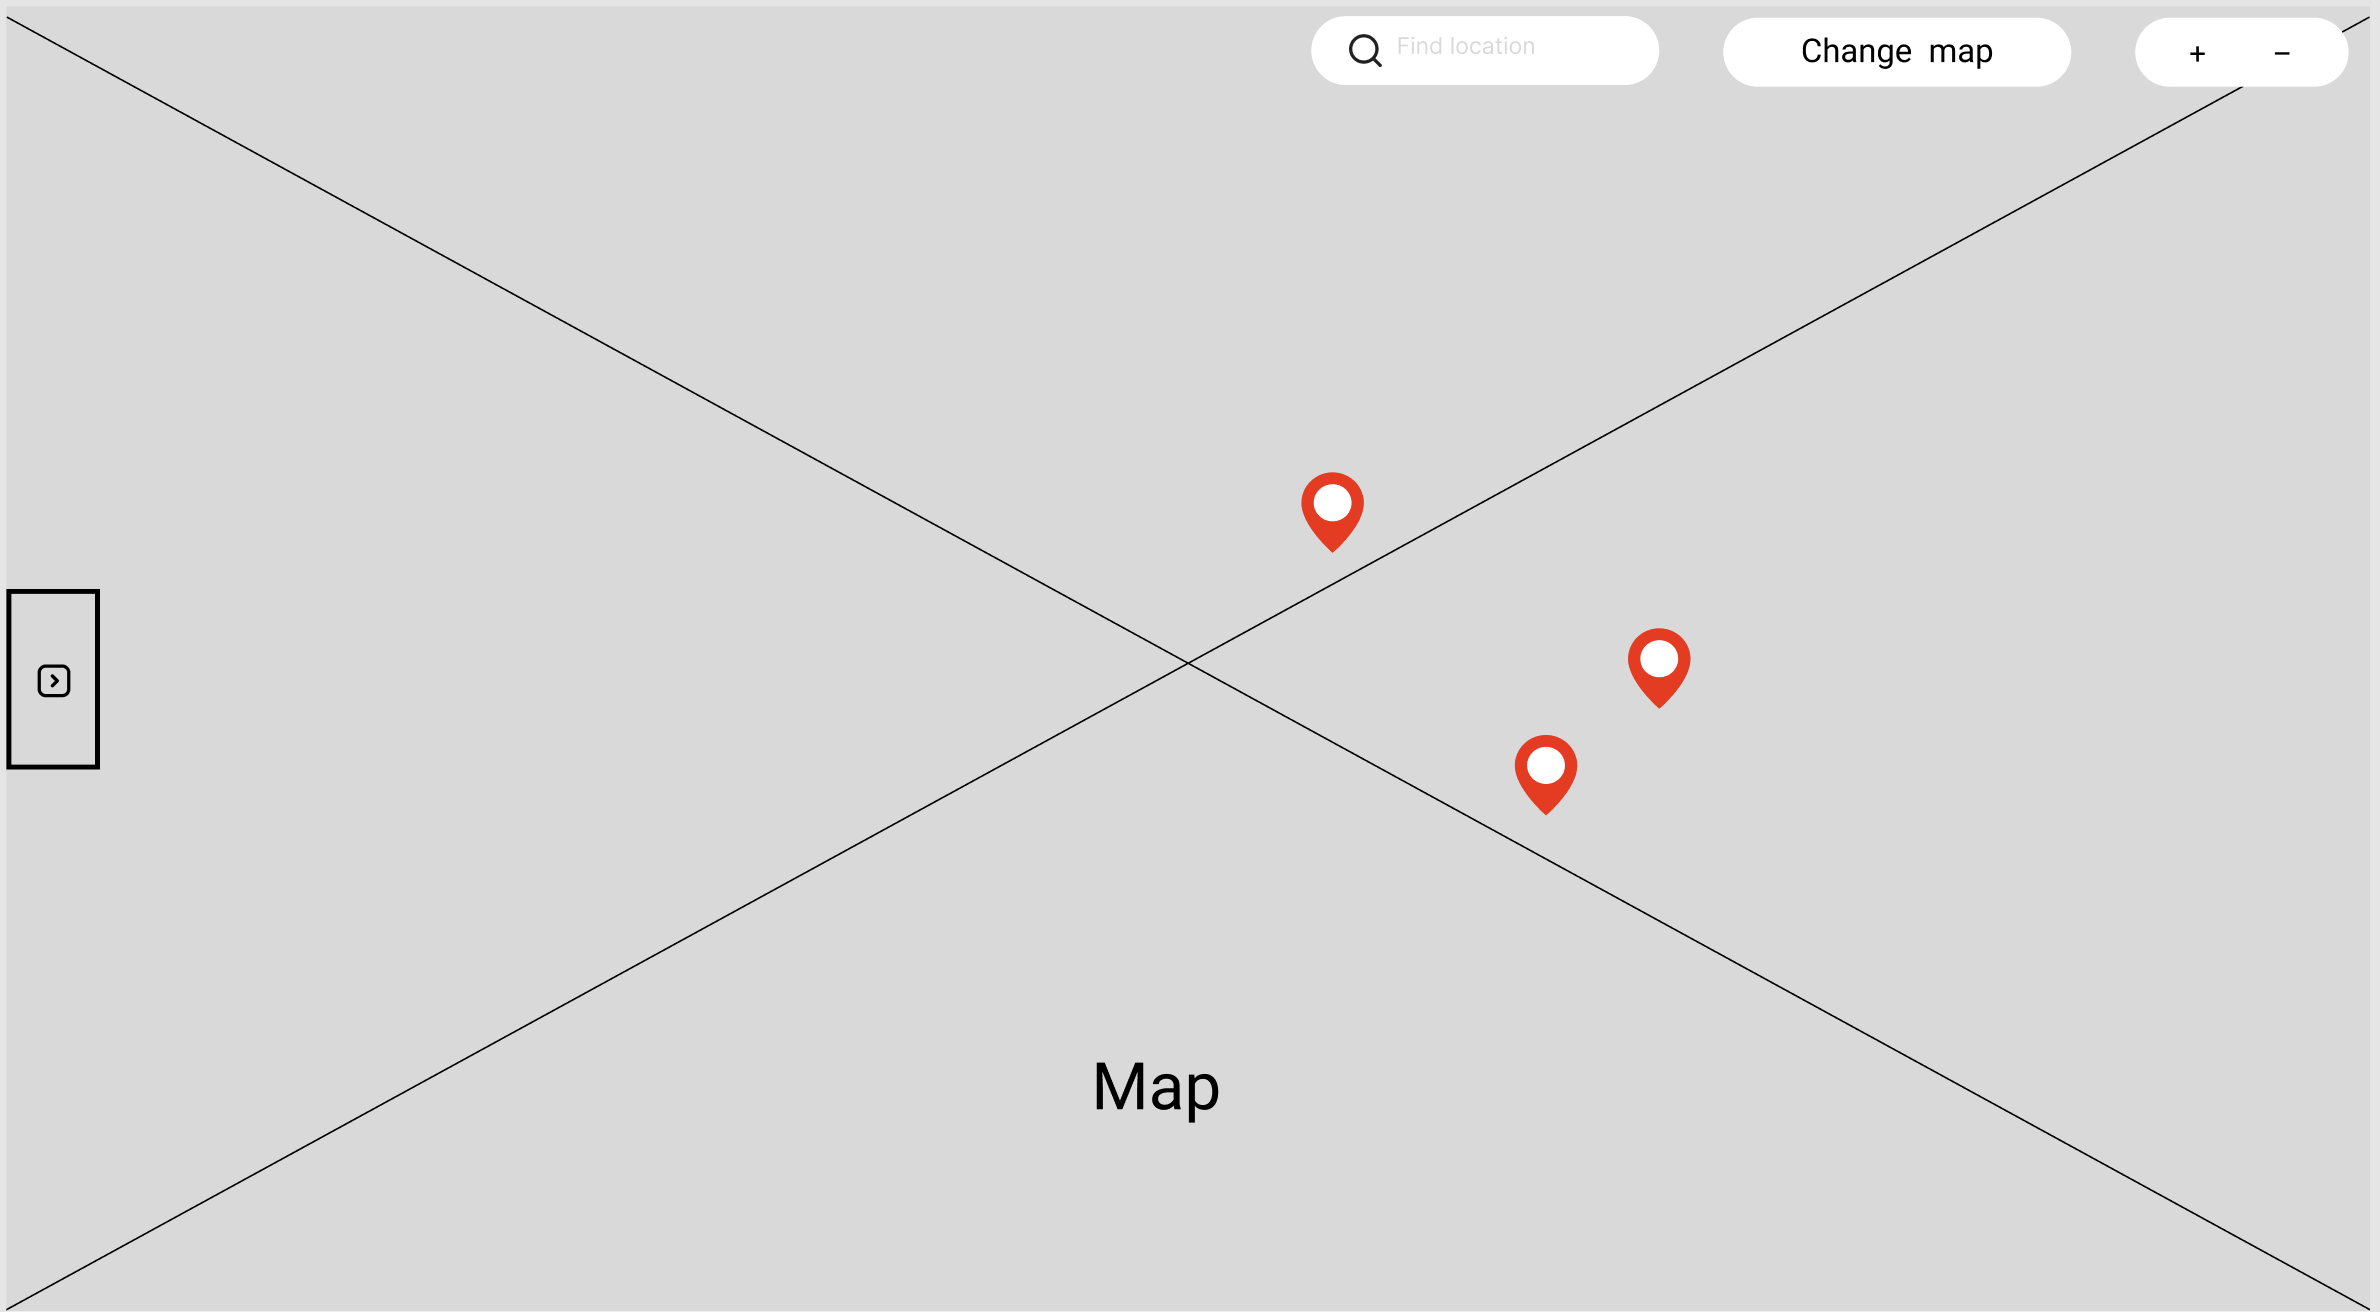
\includegraphics[width=\textwidth]{screenshot/wireframe_search.png}
    \caption{Search}
  \end{subfigure}\hfill
  \begin{subfigure}[b]{0.3\textwidth}
    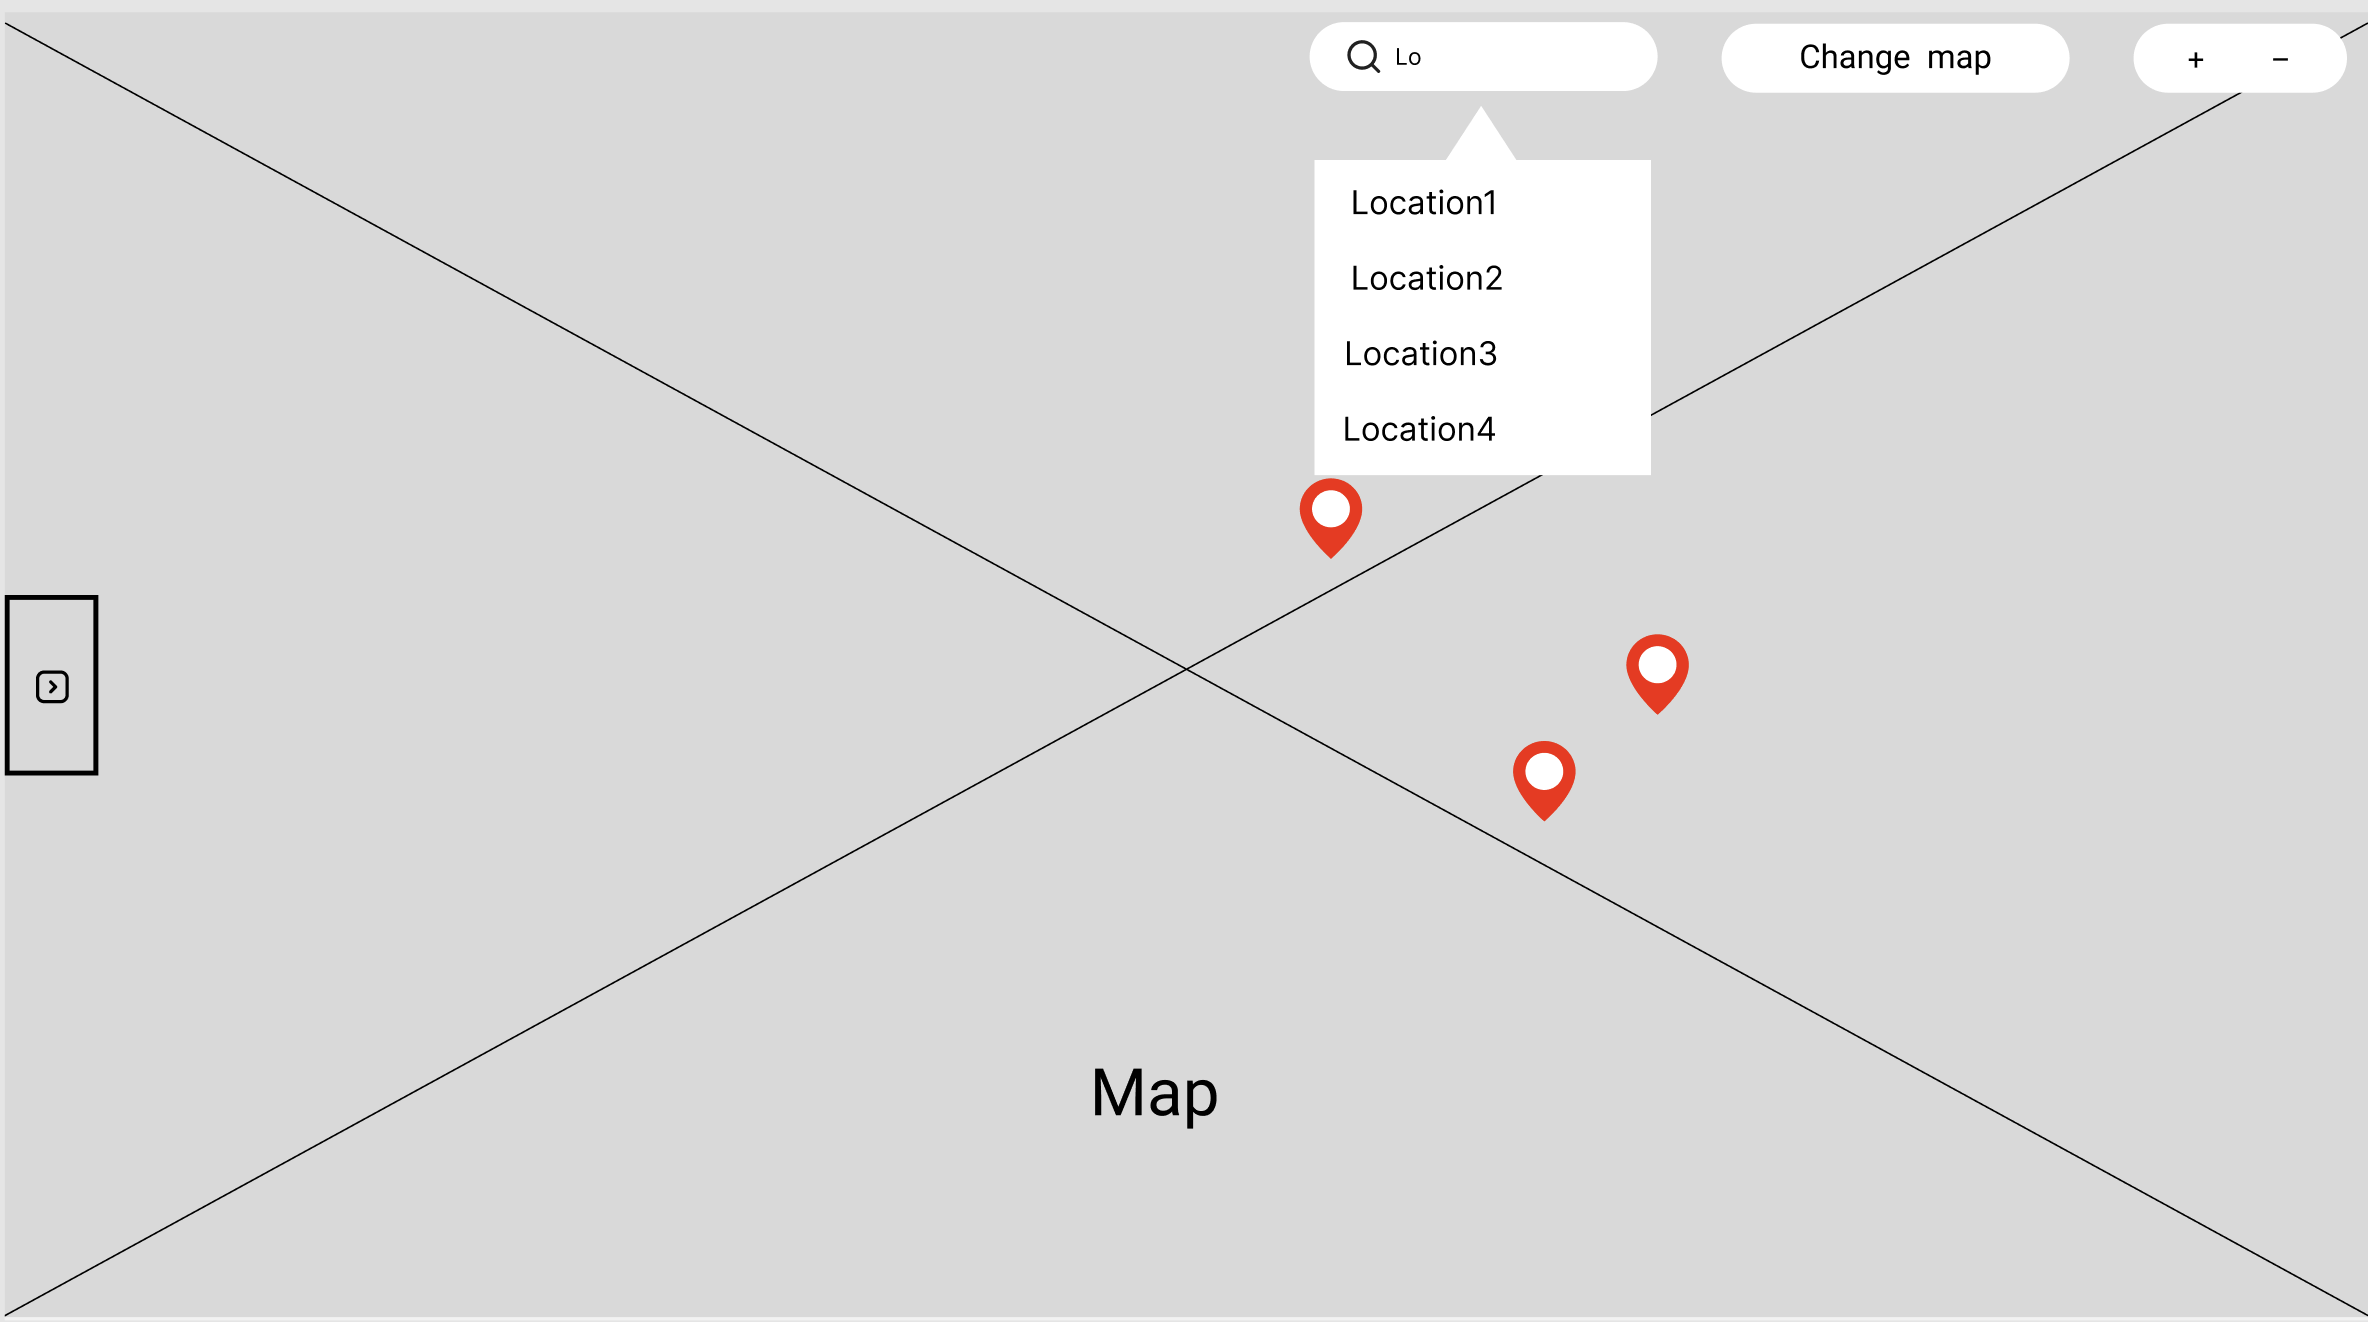
\includegraphics[width=\textwidth]{screenshot/wireframe_search2.png}
    \caption{Search 2}
  \end{subfigure}\hfill
  \begin{subfigure}[b]{0.3\textwidth}
    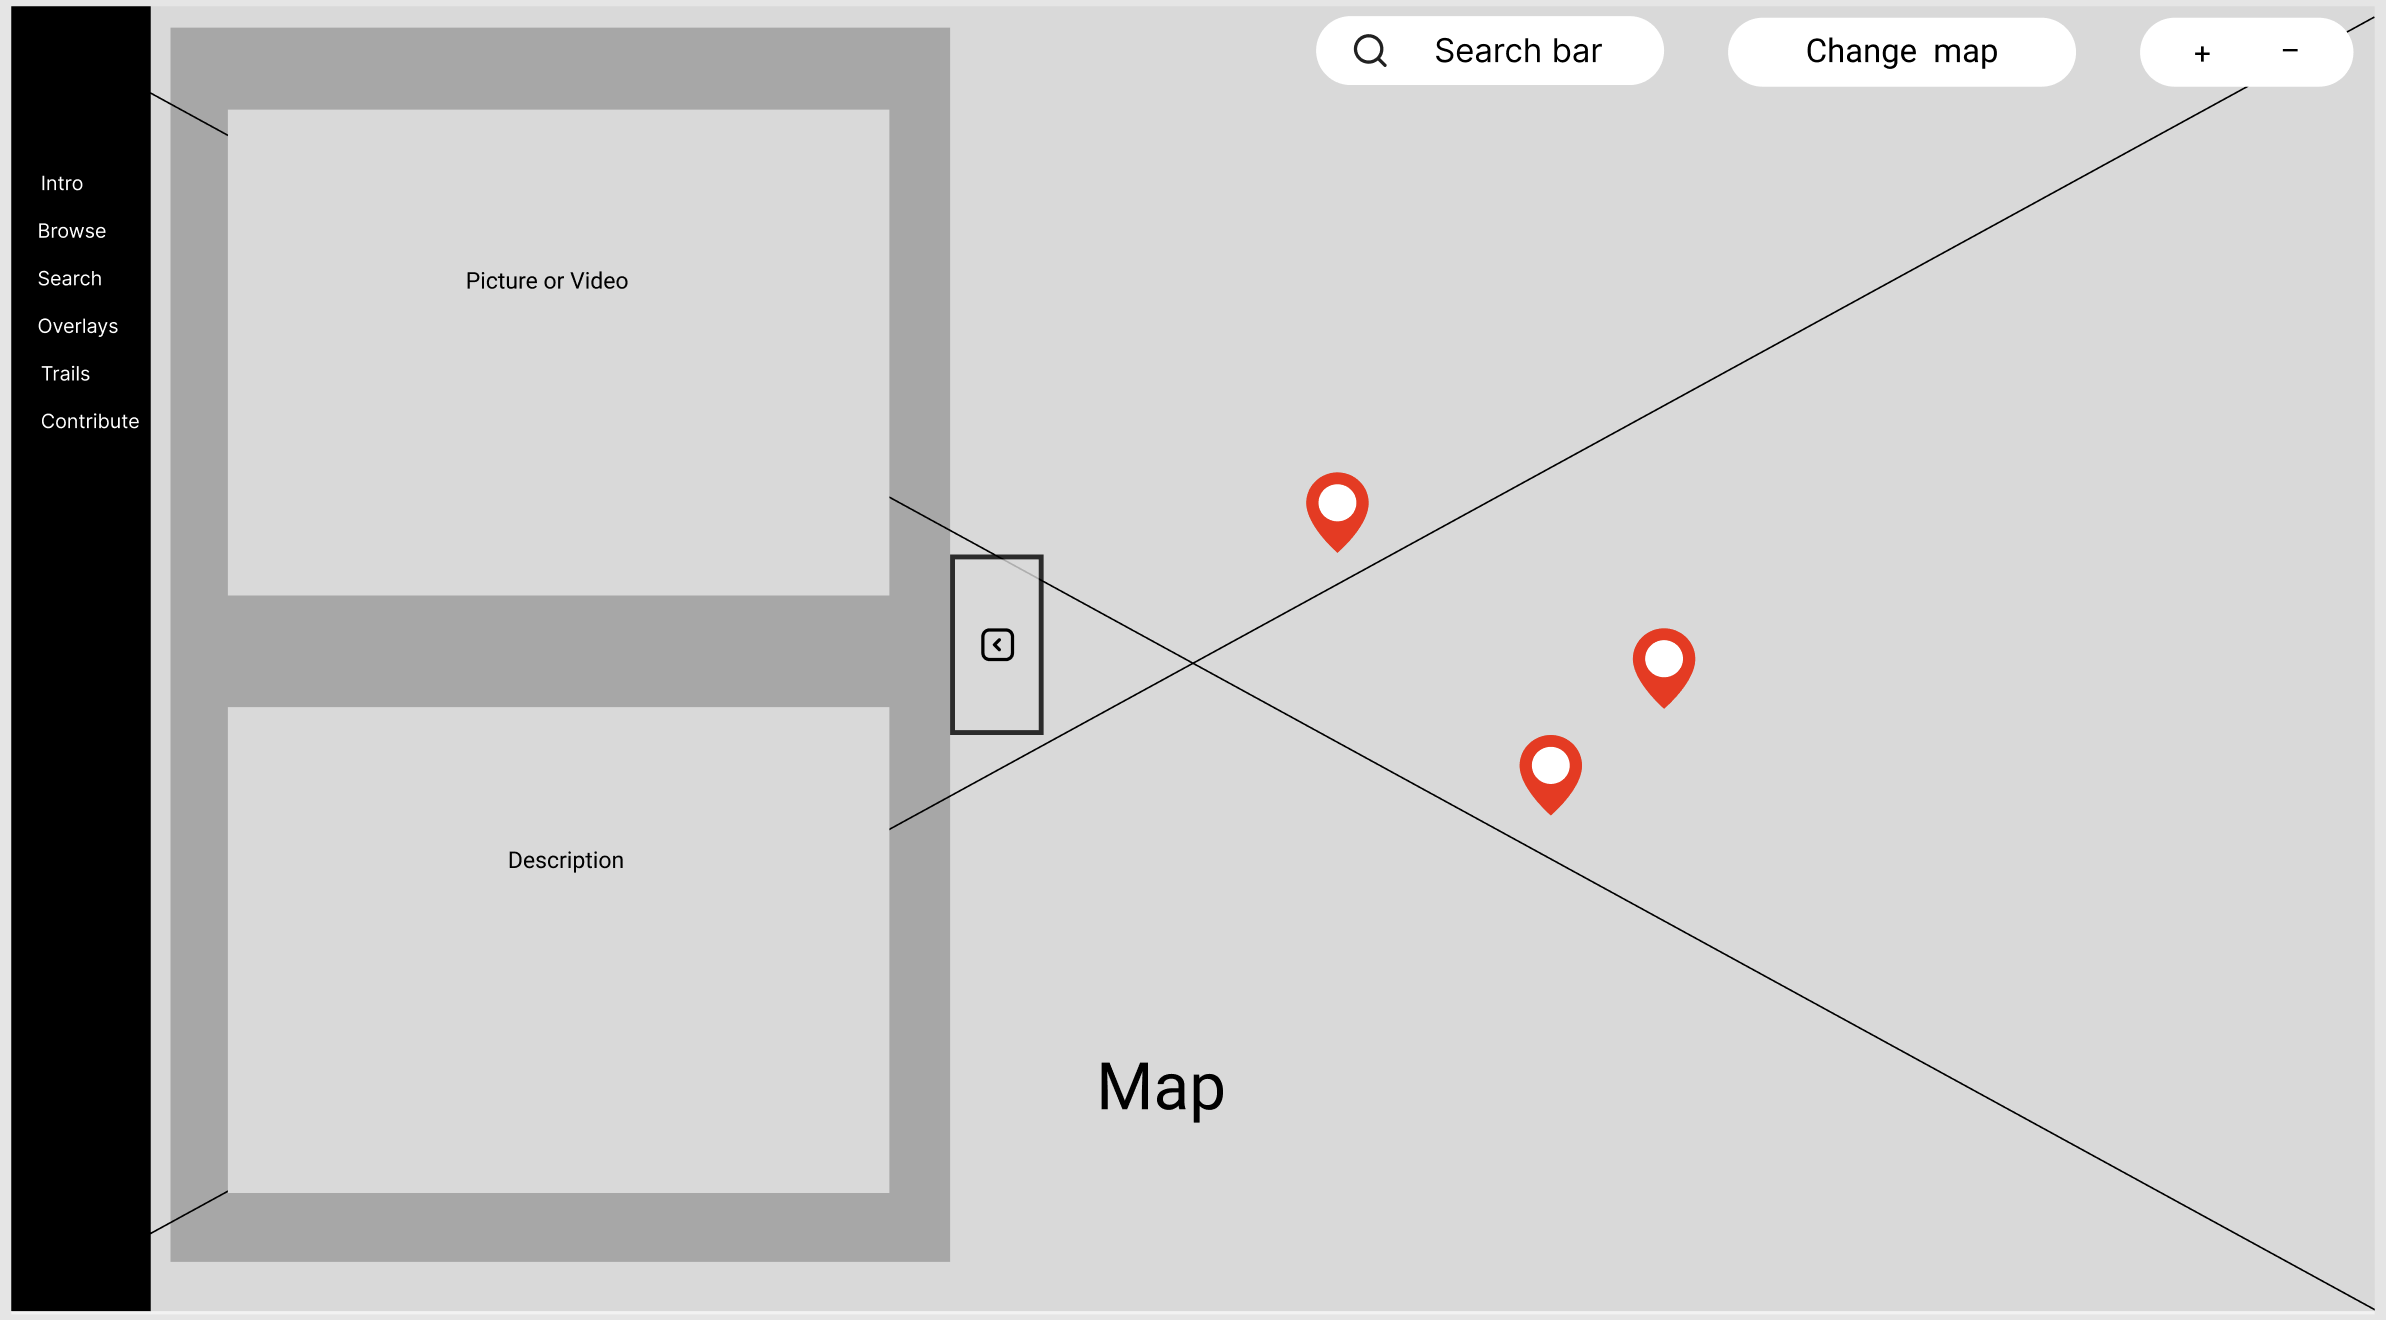
\includegraphics[width=\textwidth]{screenshot/wireframe_sidepanel.png}
    \caption{Side Panel}
  \end{subfigure}

  \vspace{0.5cm}

  % line 4
  \begin{subfigure}[b]{0.3\textwidth}
    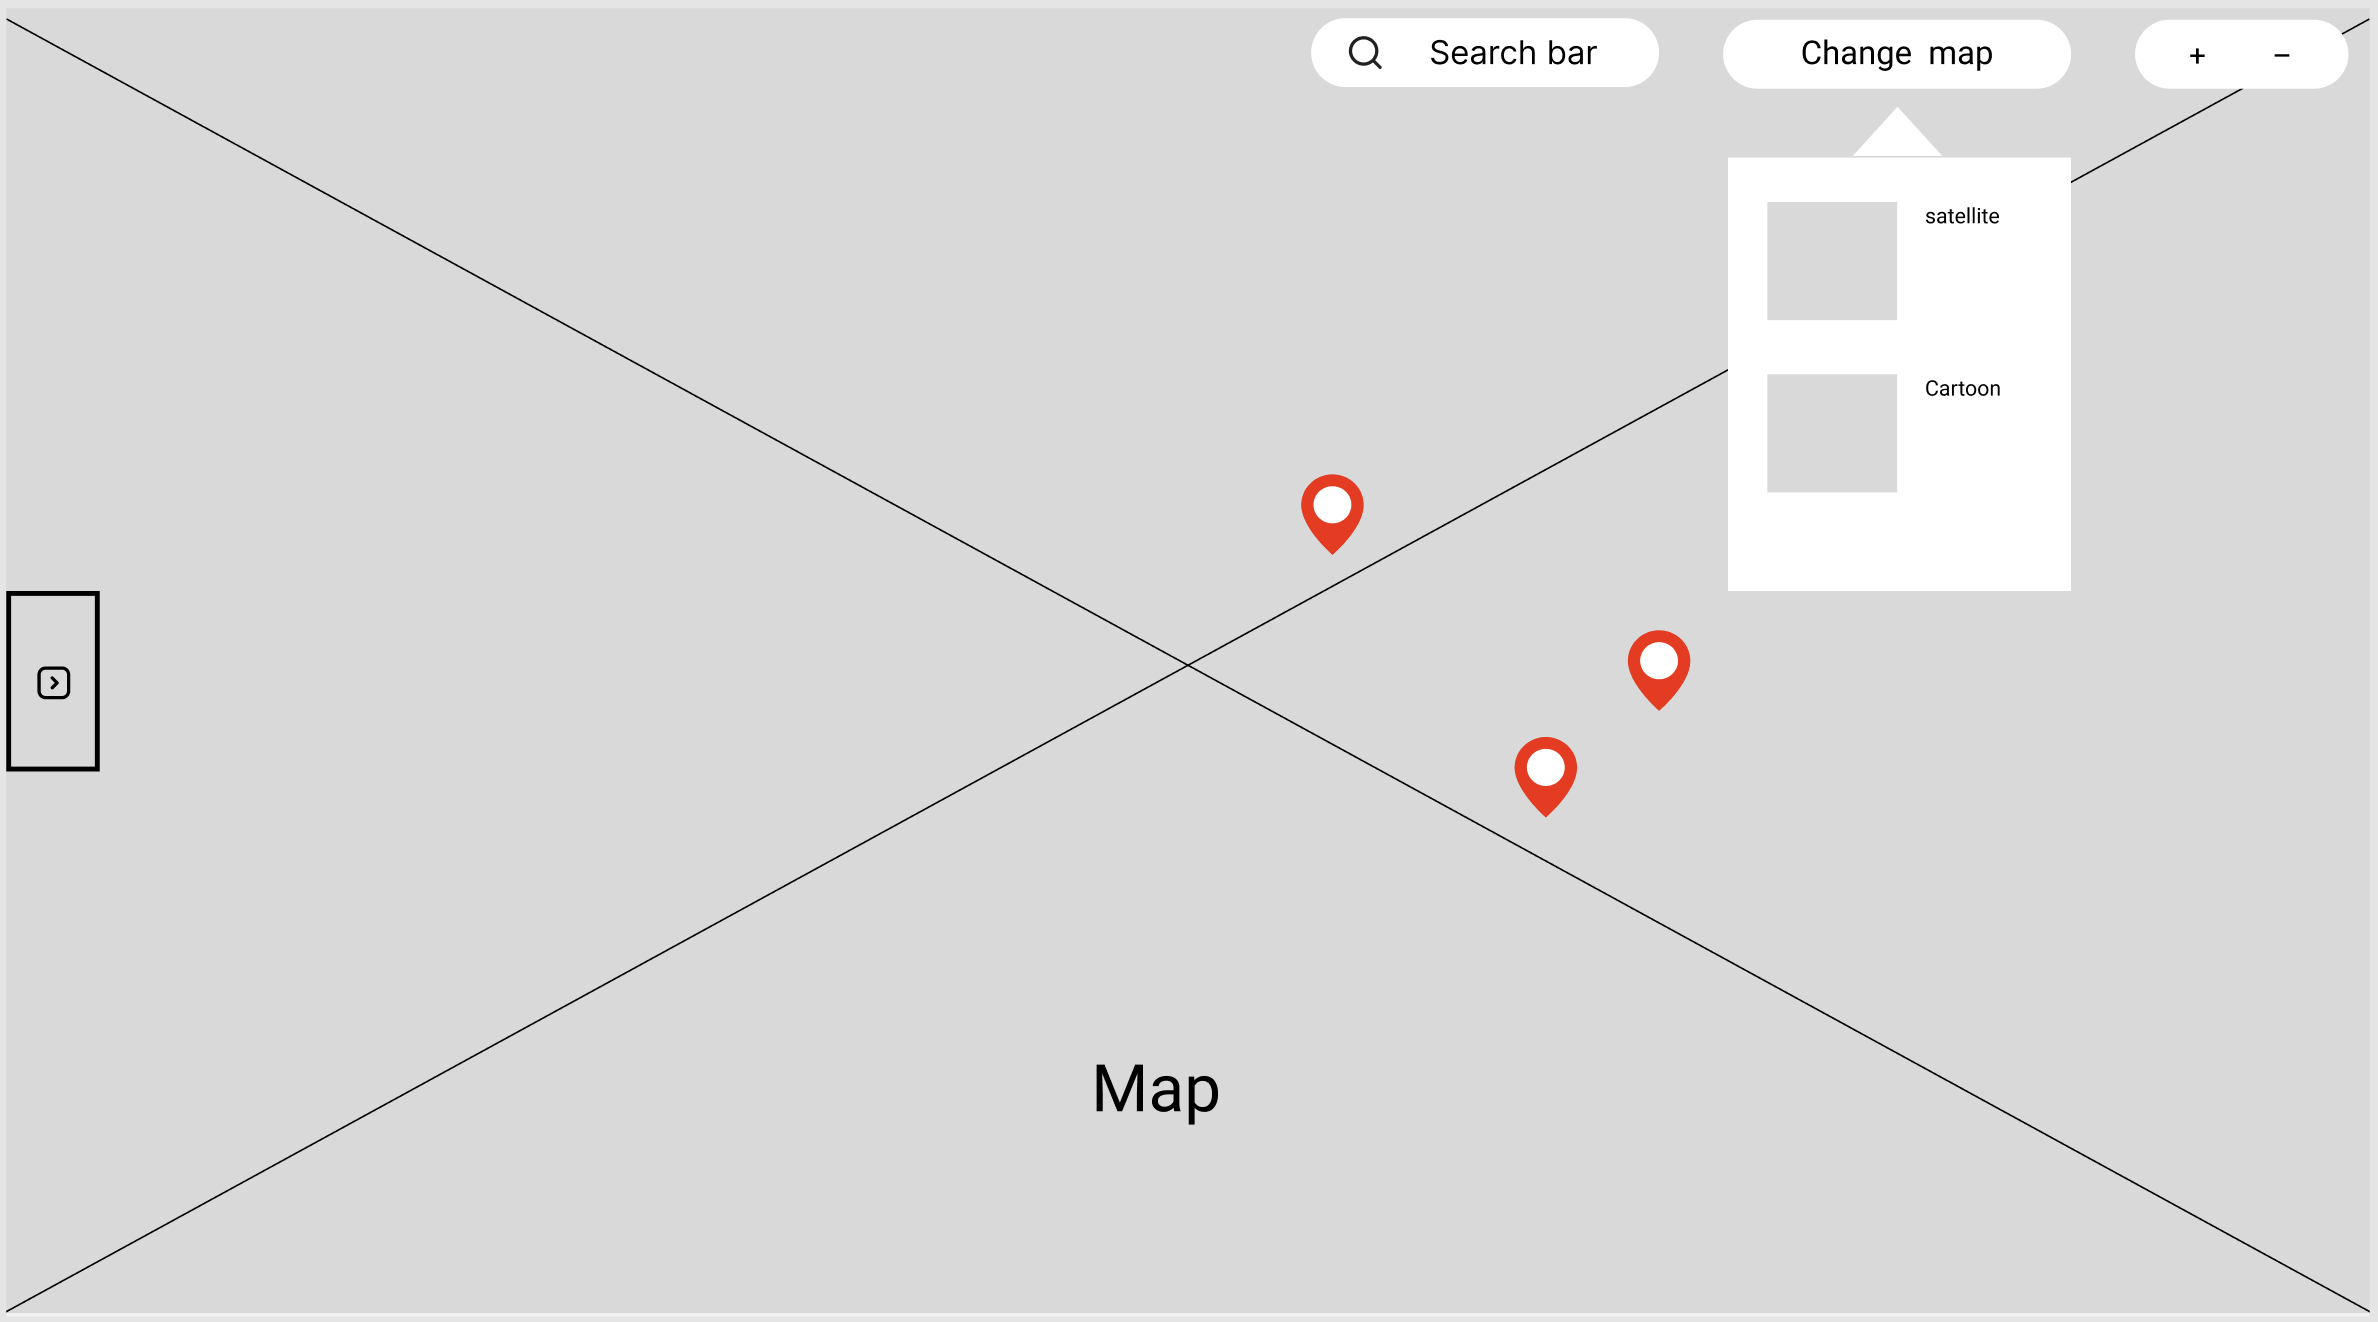
\includegraphics[width=\textwidth]{screenshot/wireframe_changemap.png}
    \caption{Change Map}
  \end{subfigure}

  \caption{Wireframe Stage Images}
  \label{fig:wireframe}
\end{figure}

% Prototype Stage
\subsection{Prototype Stage}
\begin{figure}[H]
  \centering
  % line 1
  \begin{subfigure}[b]{0.3\textwidth}
    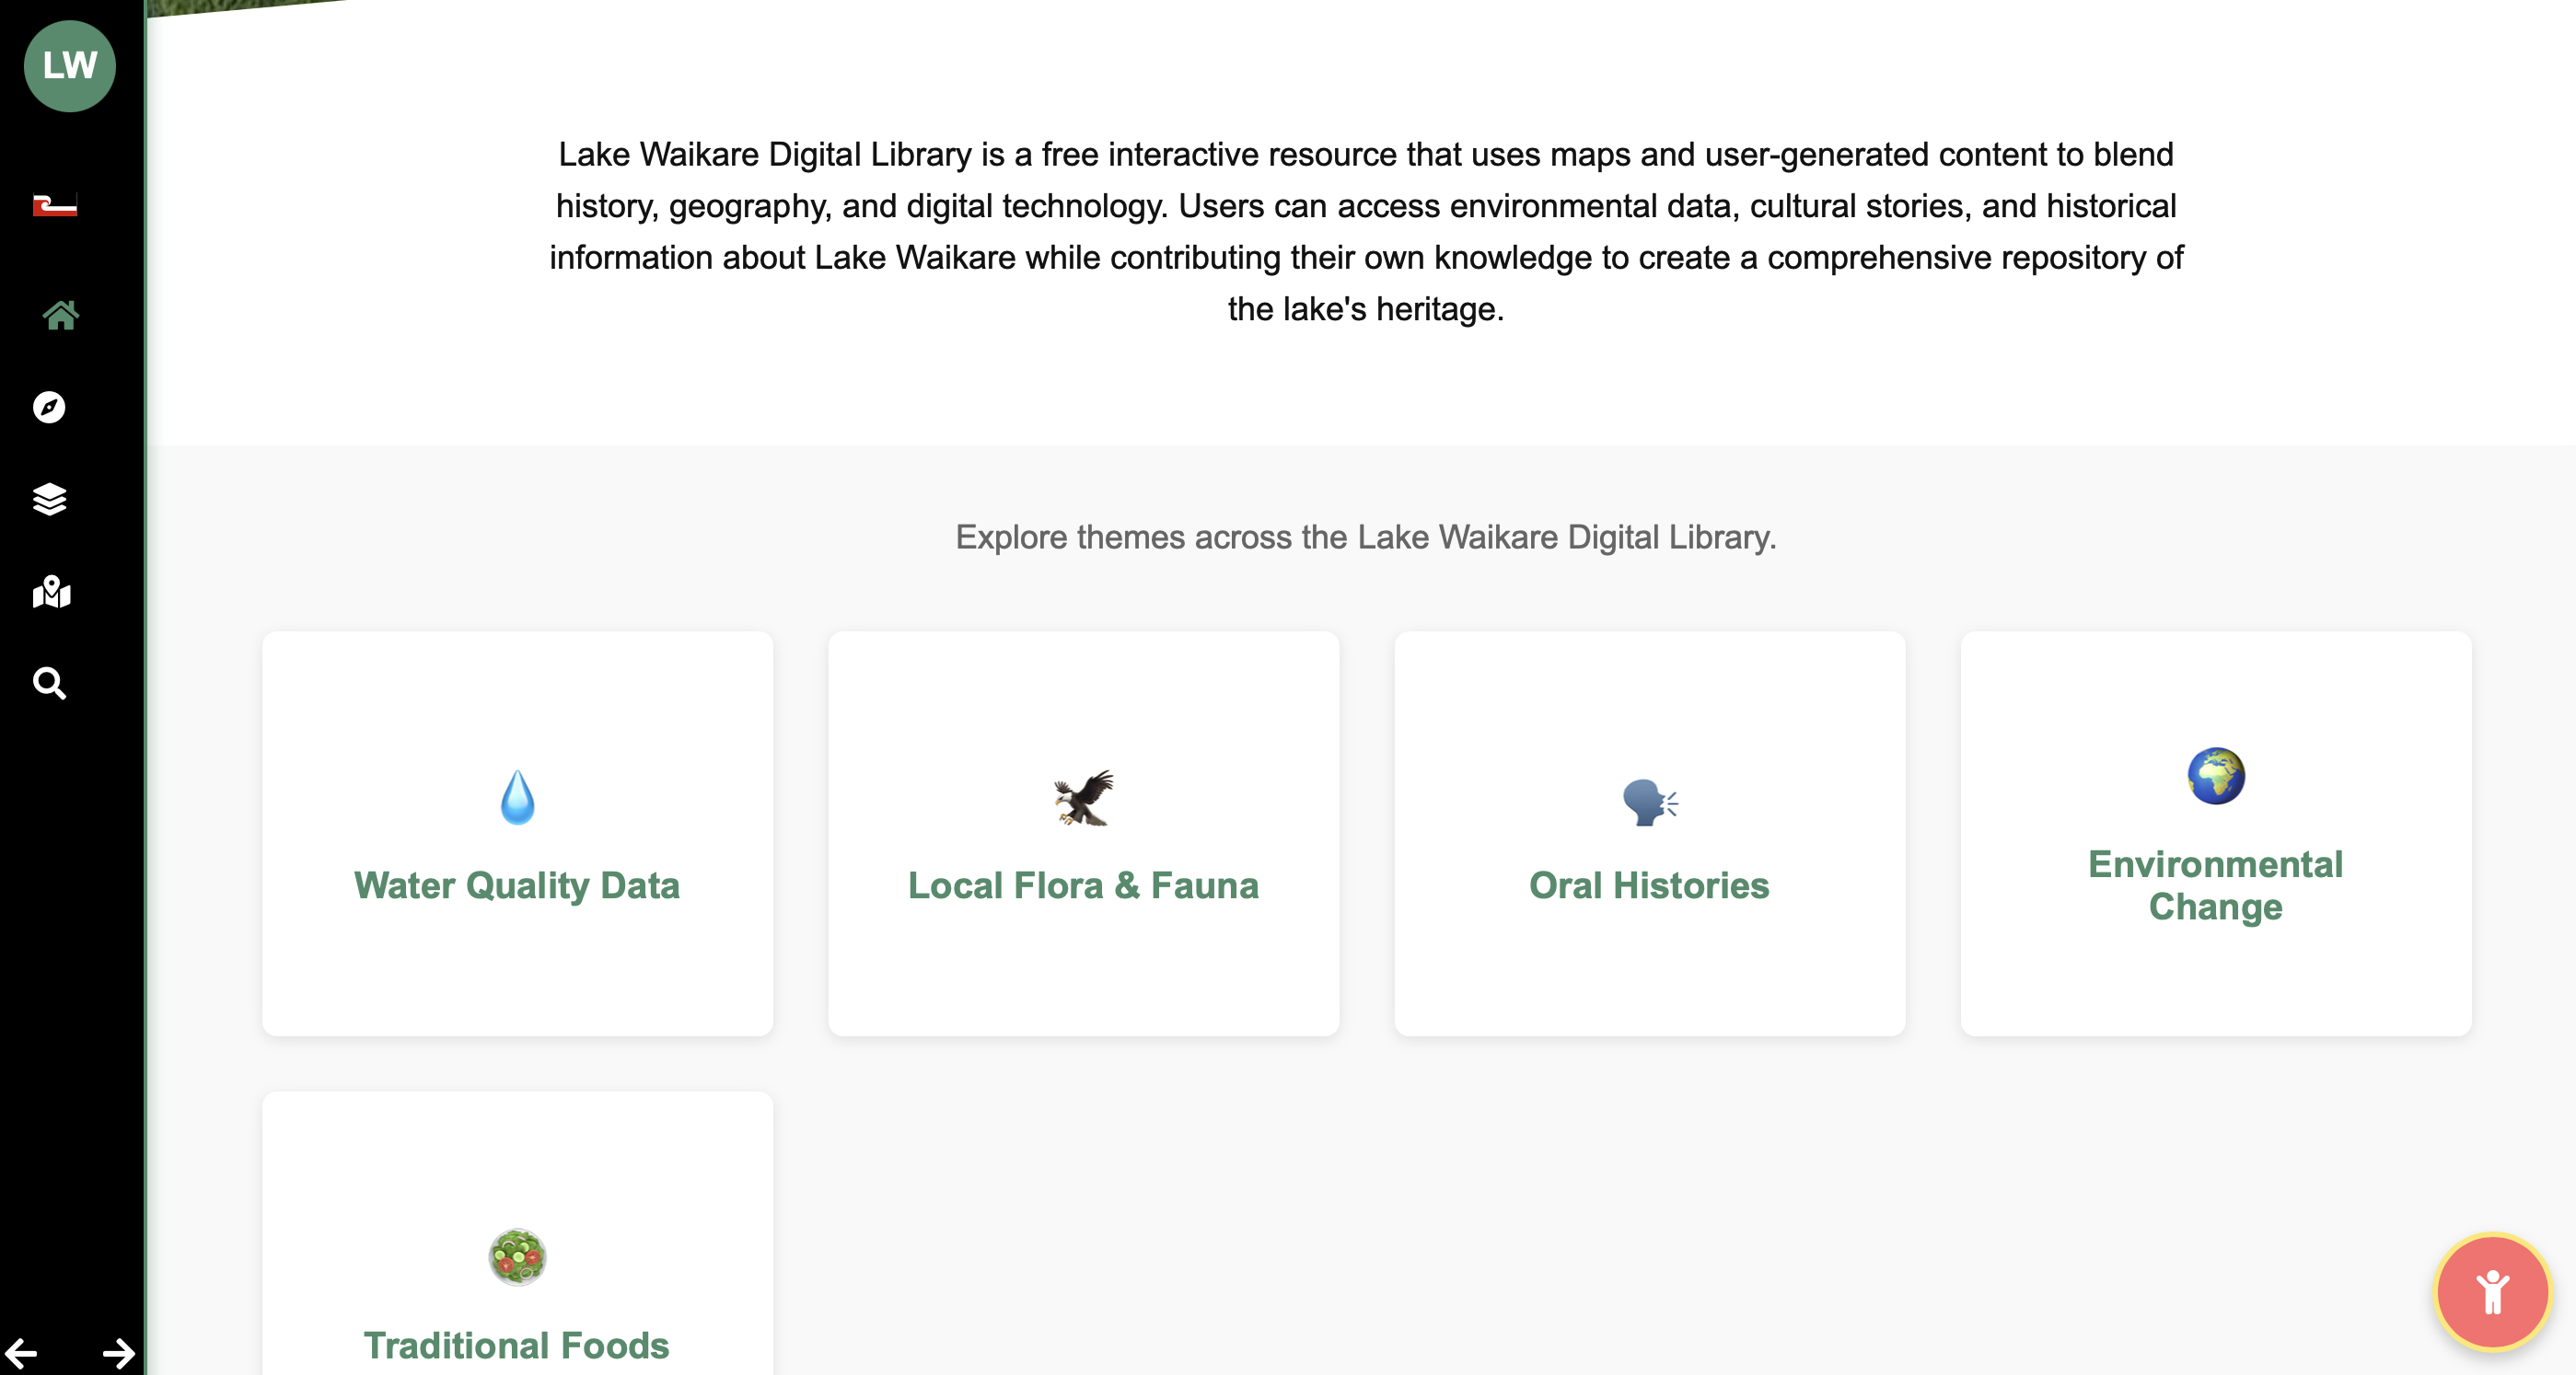
\includegraphics[width=\textwidth]{screenshot/prototype_main1.png}
    \caption{Main 1}
  \end{subfigure}\hfill
  \begin{subfigure}[b]{0.3\textwidth}
    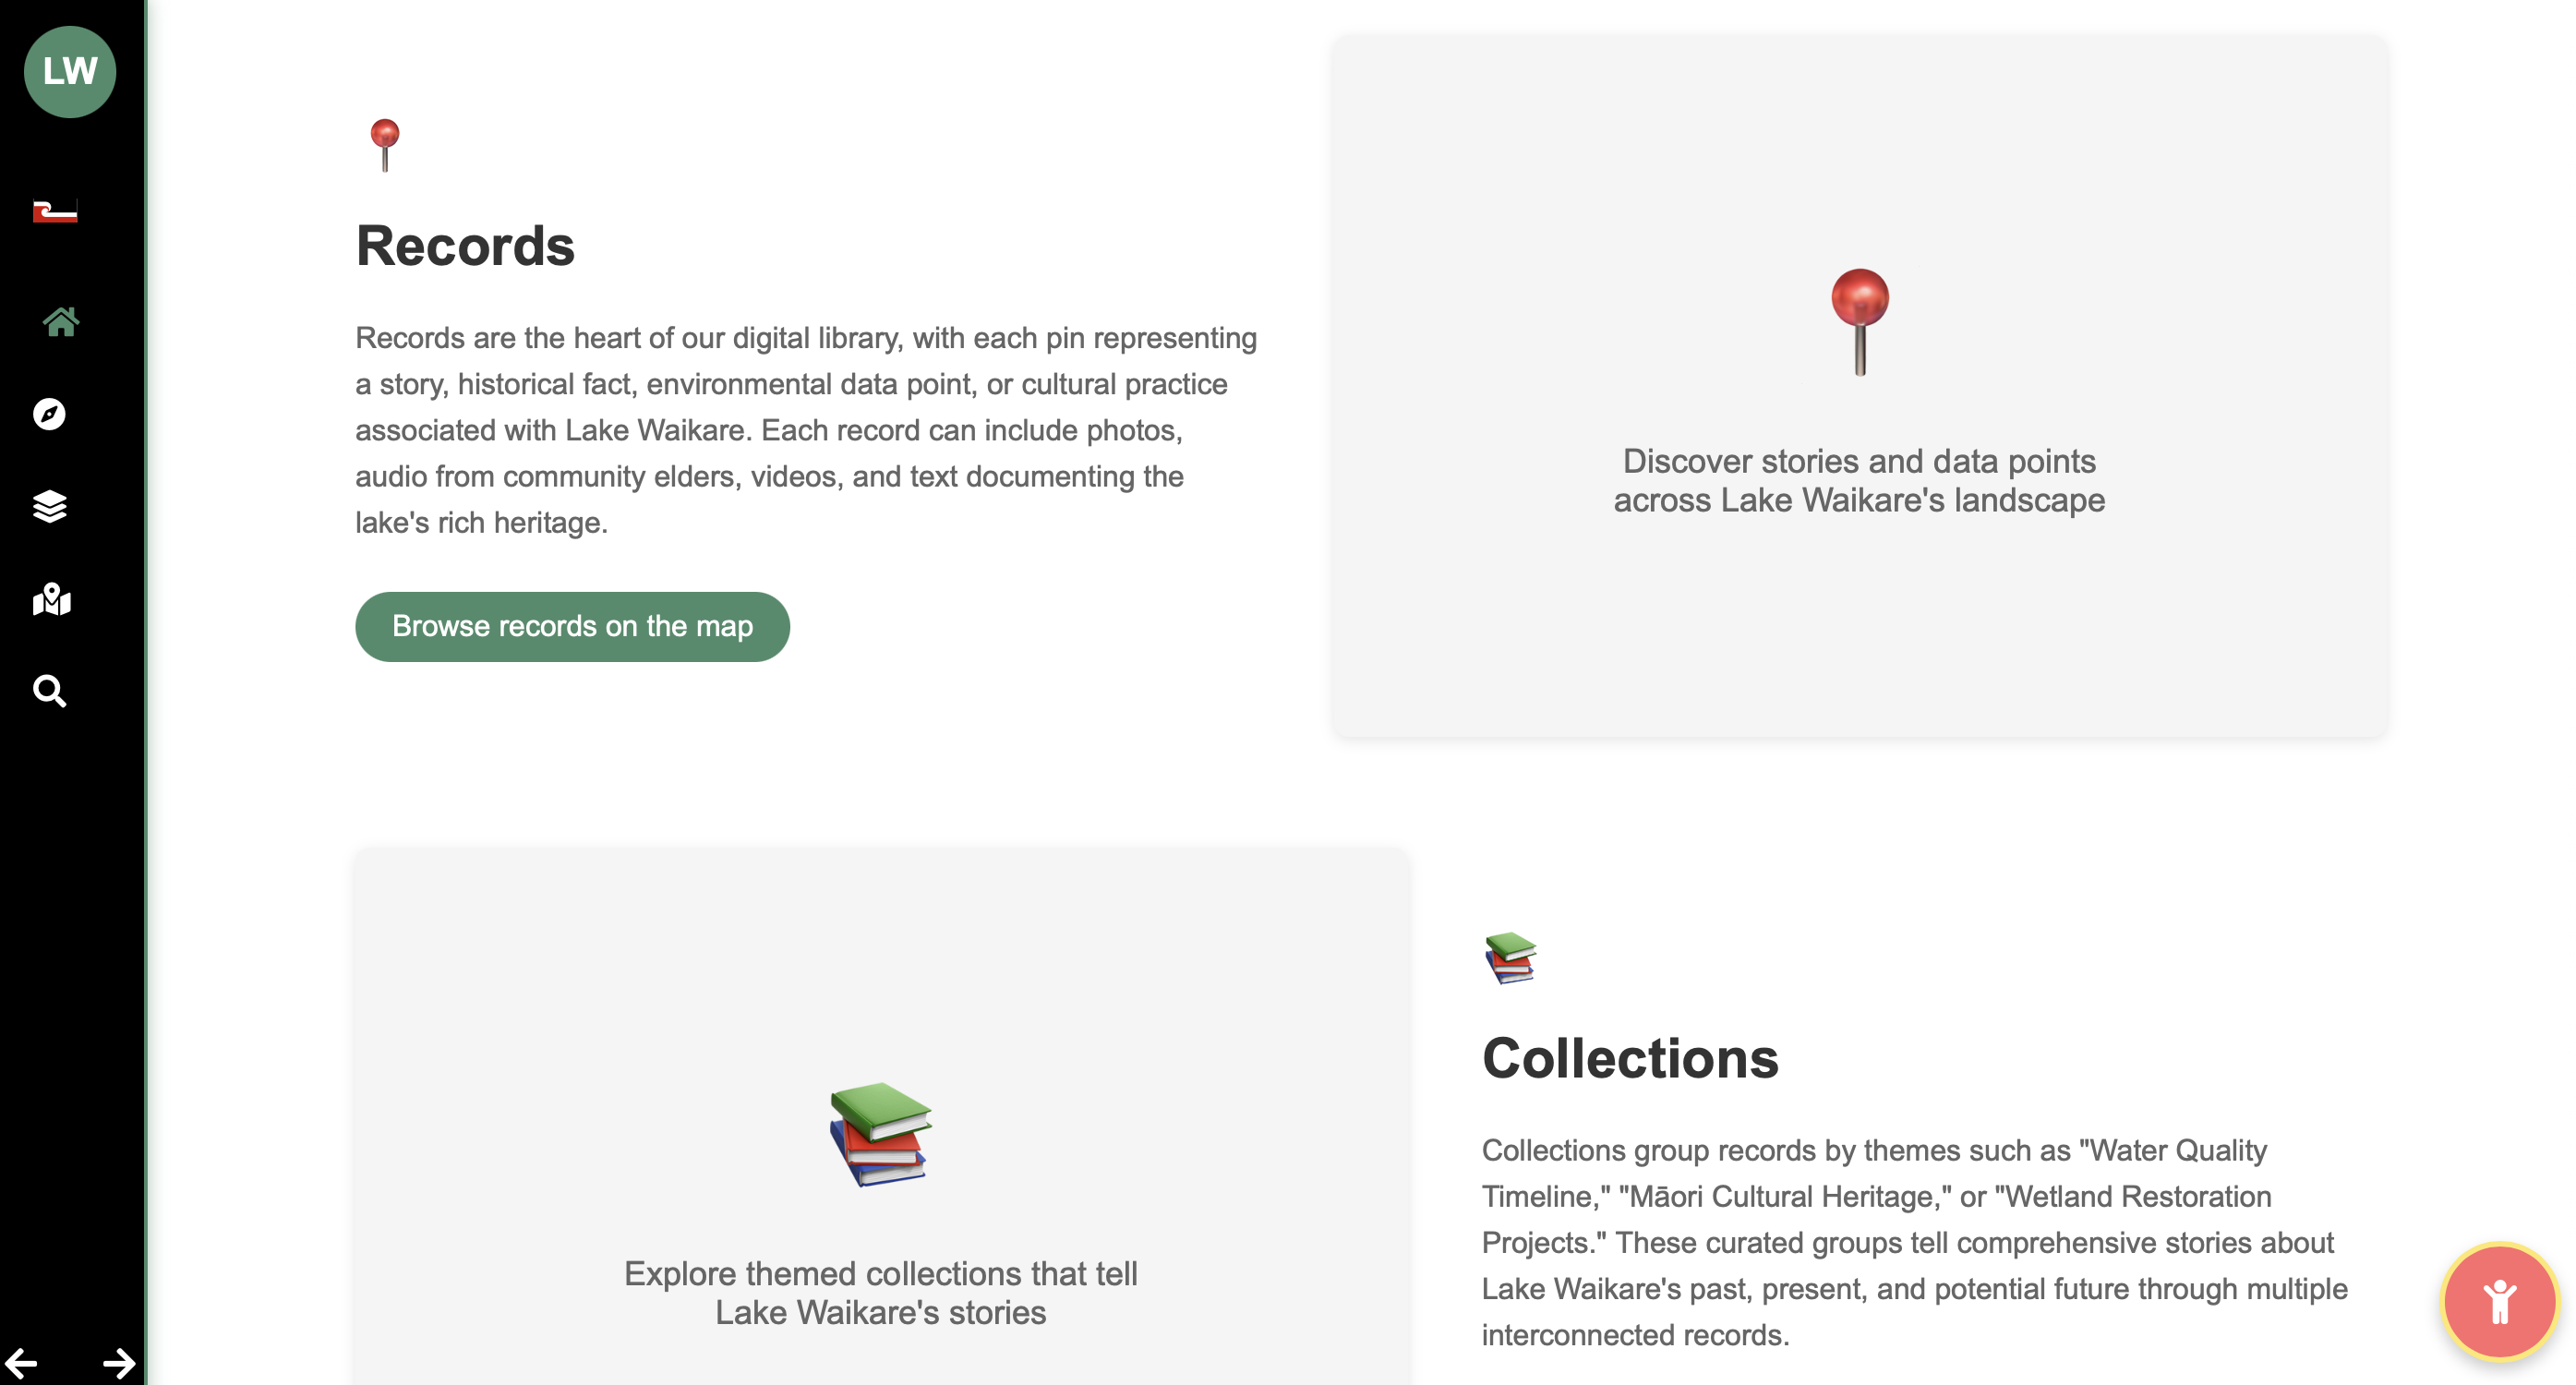
\includegraphics[width=\textwidth]{screenshot/prototype_main2.png}
    \caption{Main 2}
  \end{subfigure}\hfill
  \begin{subfigure}[b]{0.3\textwidth}
    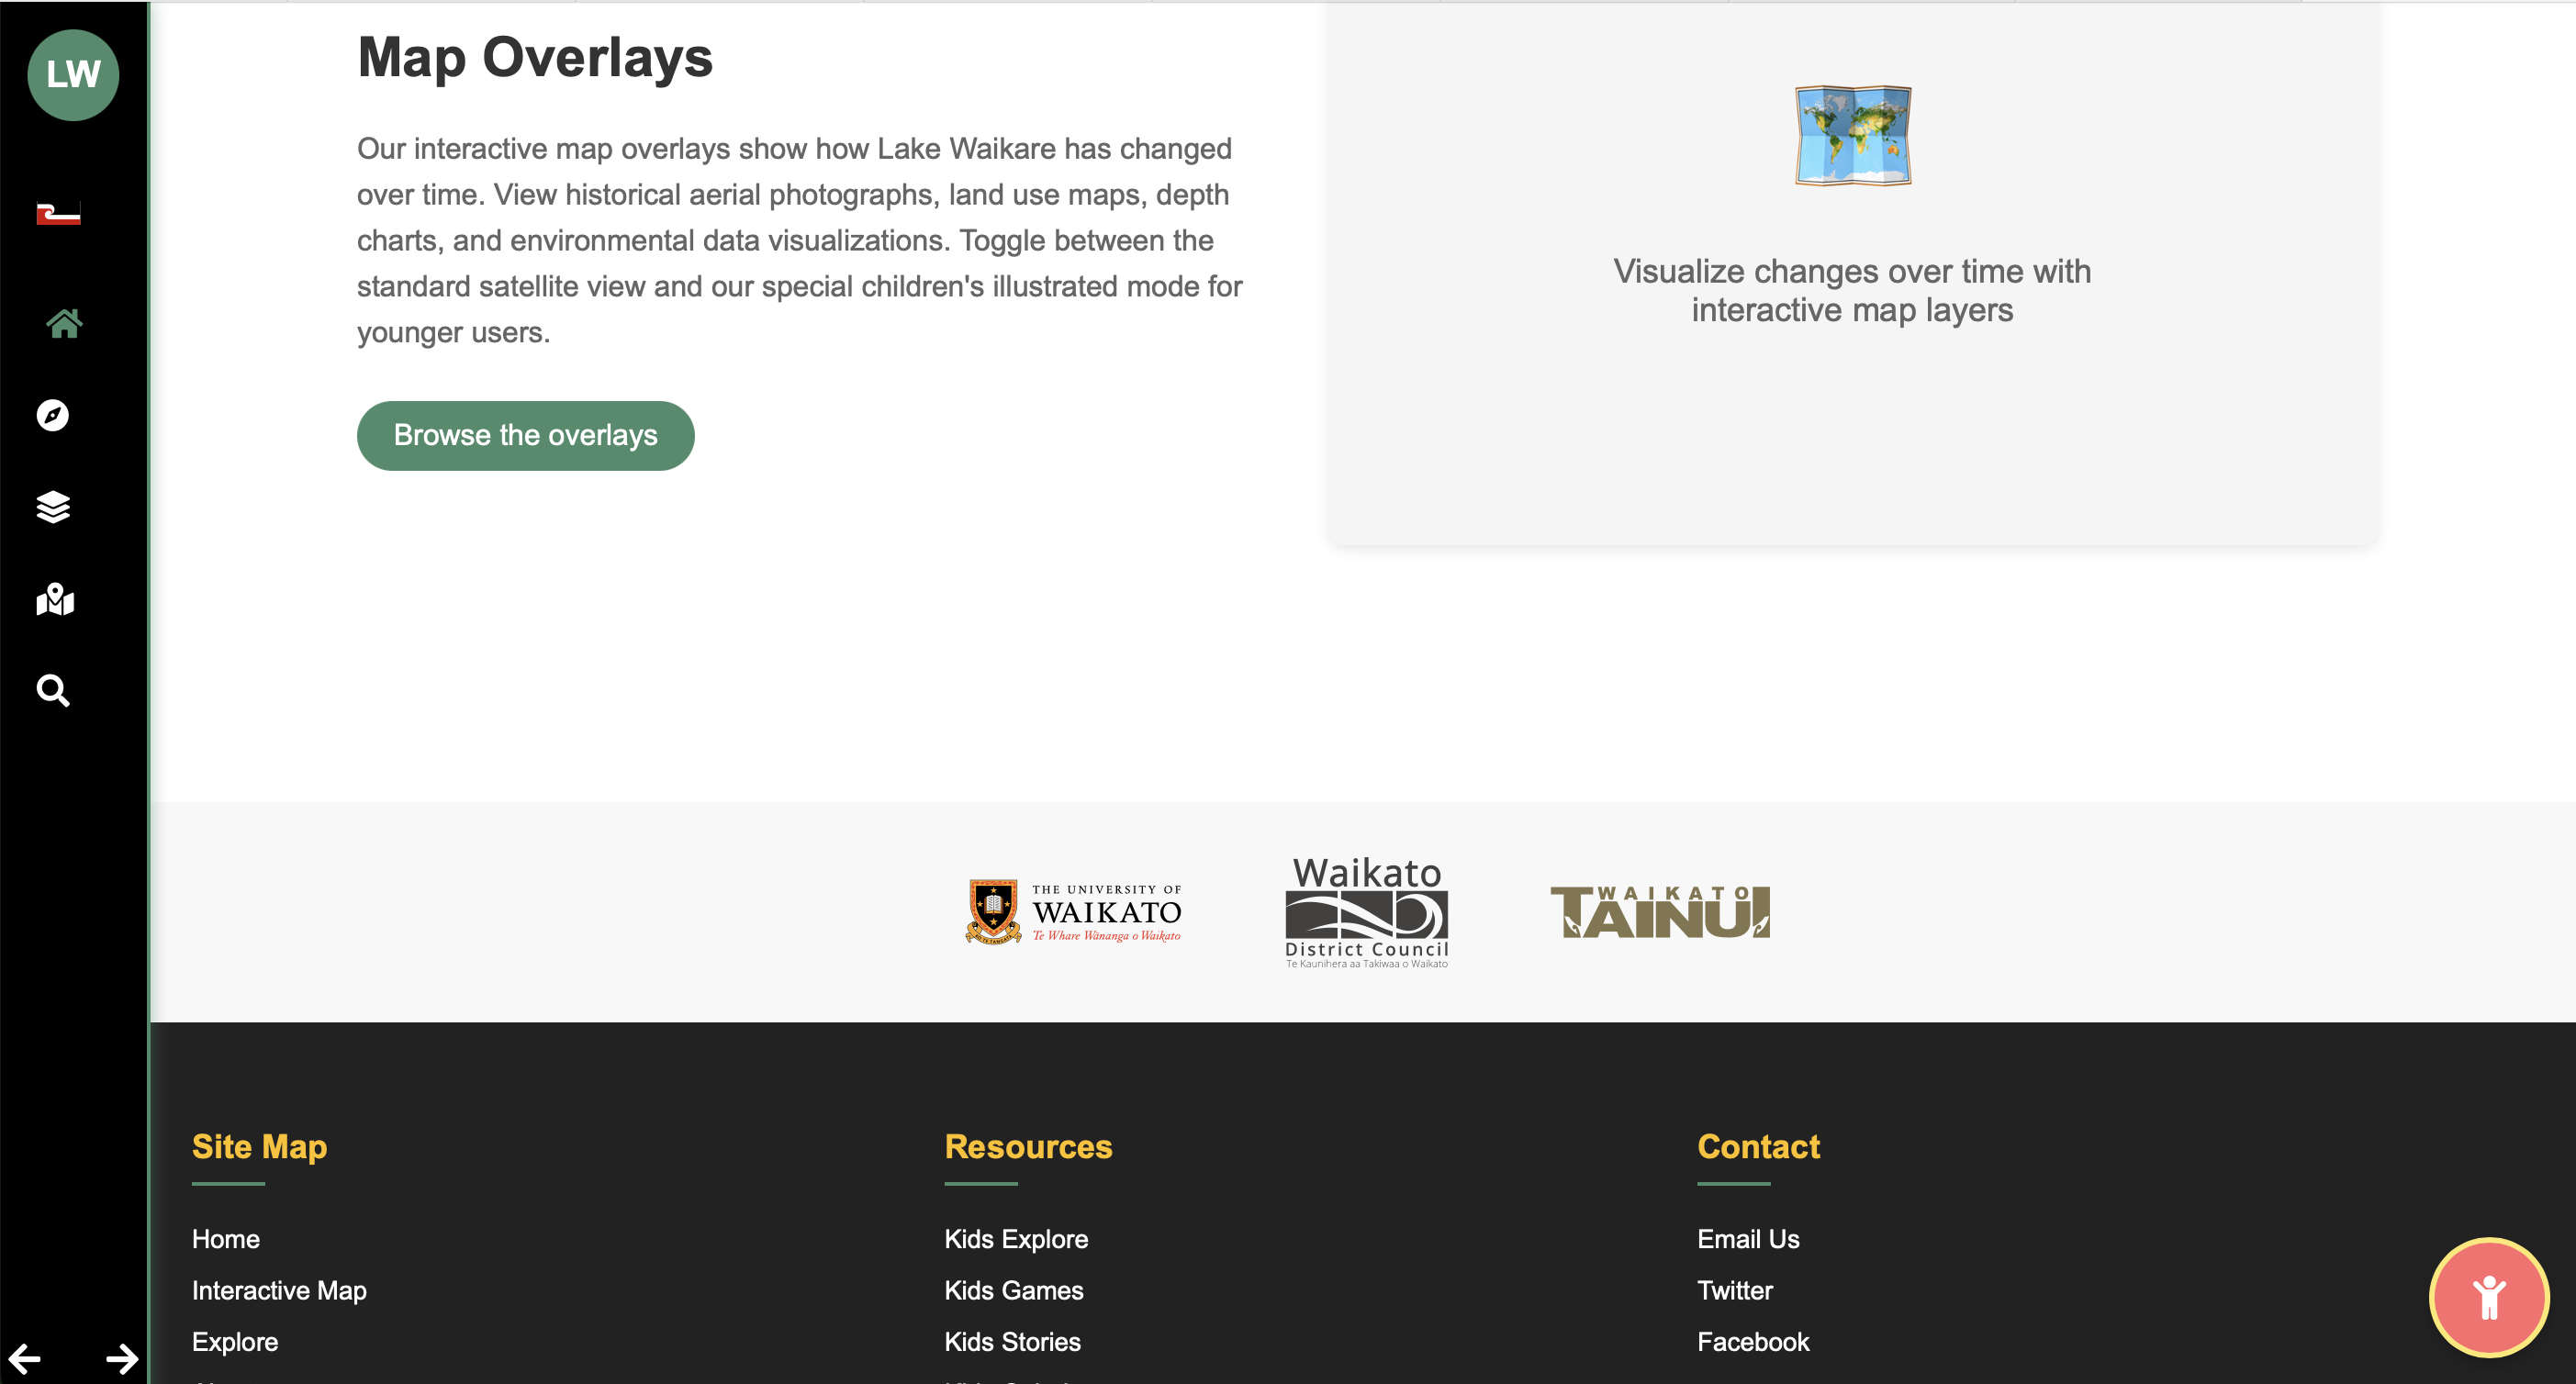
\includegraphics[width=\textwidth]{screenshot/prototype_main3.png}
    \caption{Main 3}
  \end{subfigure}

  \vspace{0.5cm}

  % line 2
  \begin{subfigure}[b]{0.3\textwidth}
    \includegraphics[width=\textwidth]{screenshot/prototype_maori_language.png}
    \caption{Maori Language}
  \end{subfigure}\hfill
  \begin{subfigure}[b]{0.3\textwidth}
    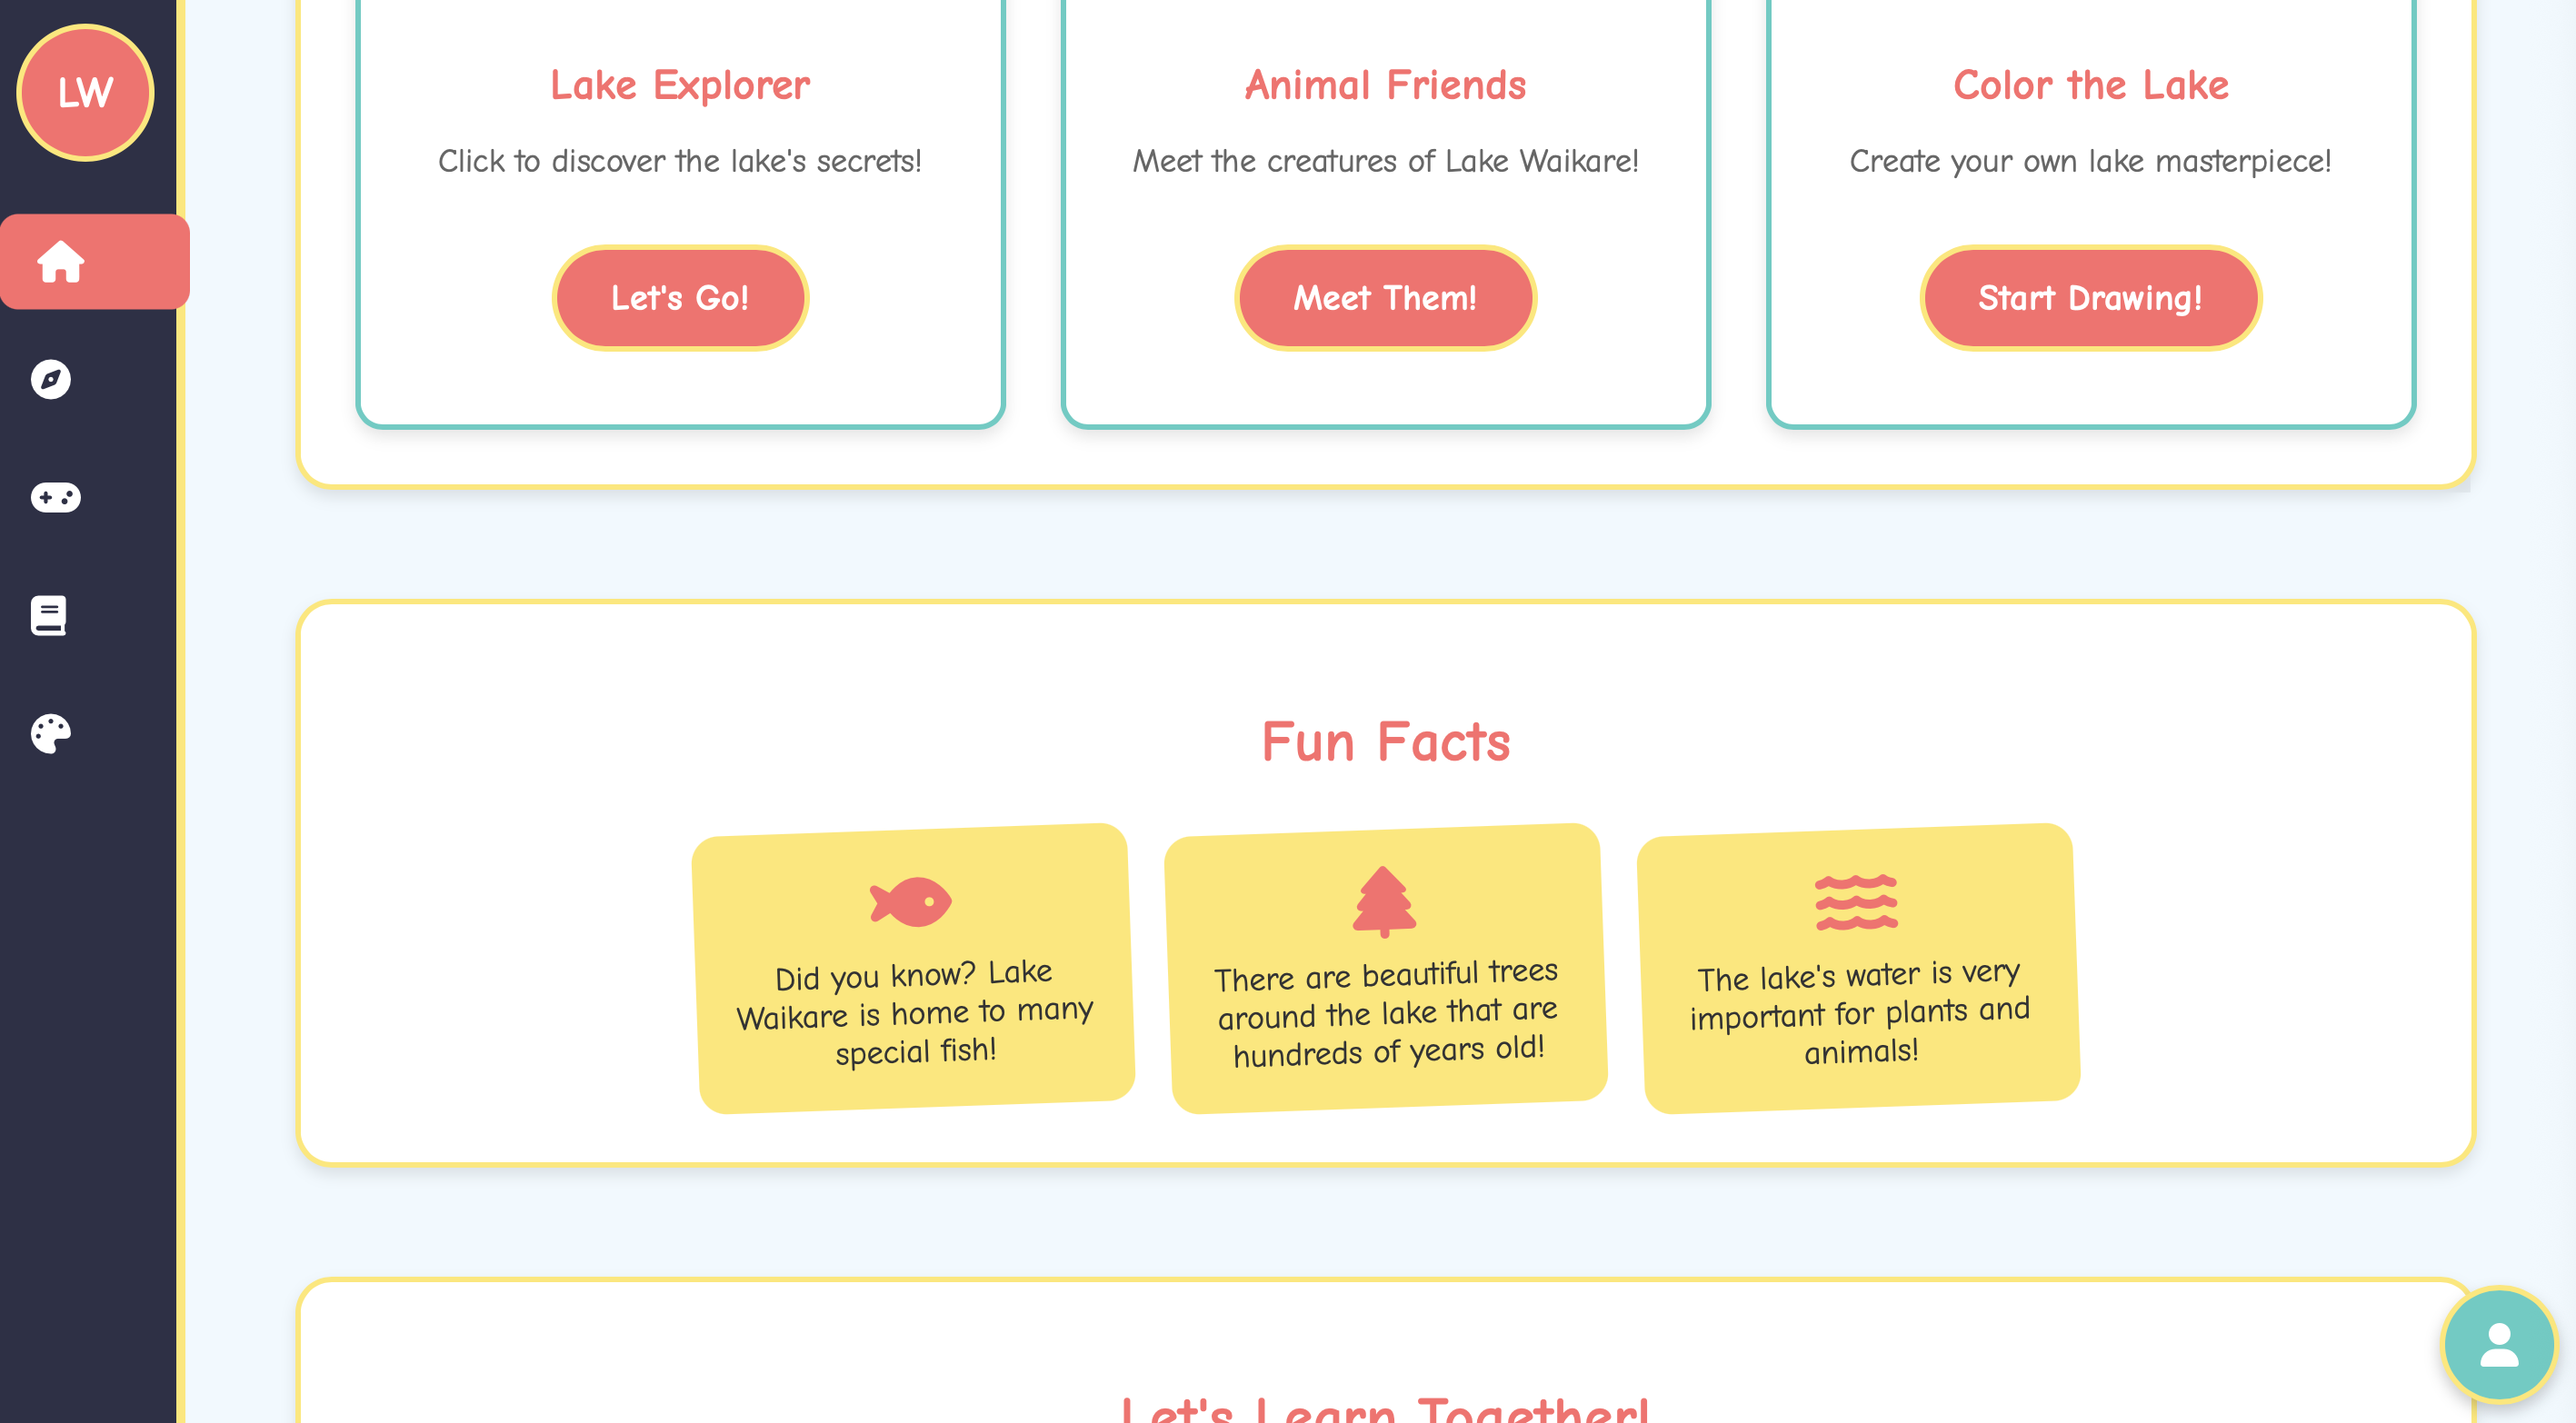
\includegraphics[width=\textwidth]{screenshot/prototype_childmode.png}
    \caption{Child Mode}
  \end{subfigure}\hfill
  \begin{subfigure}[b]{0.3\textwidth}
    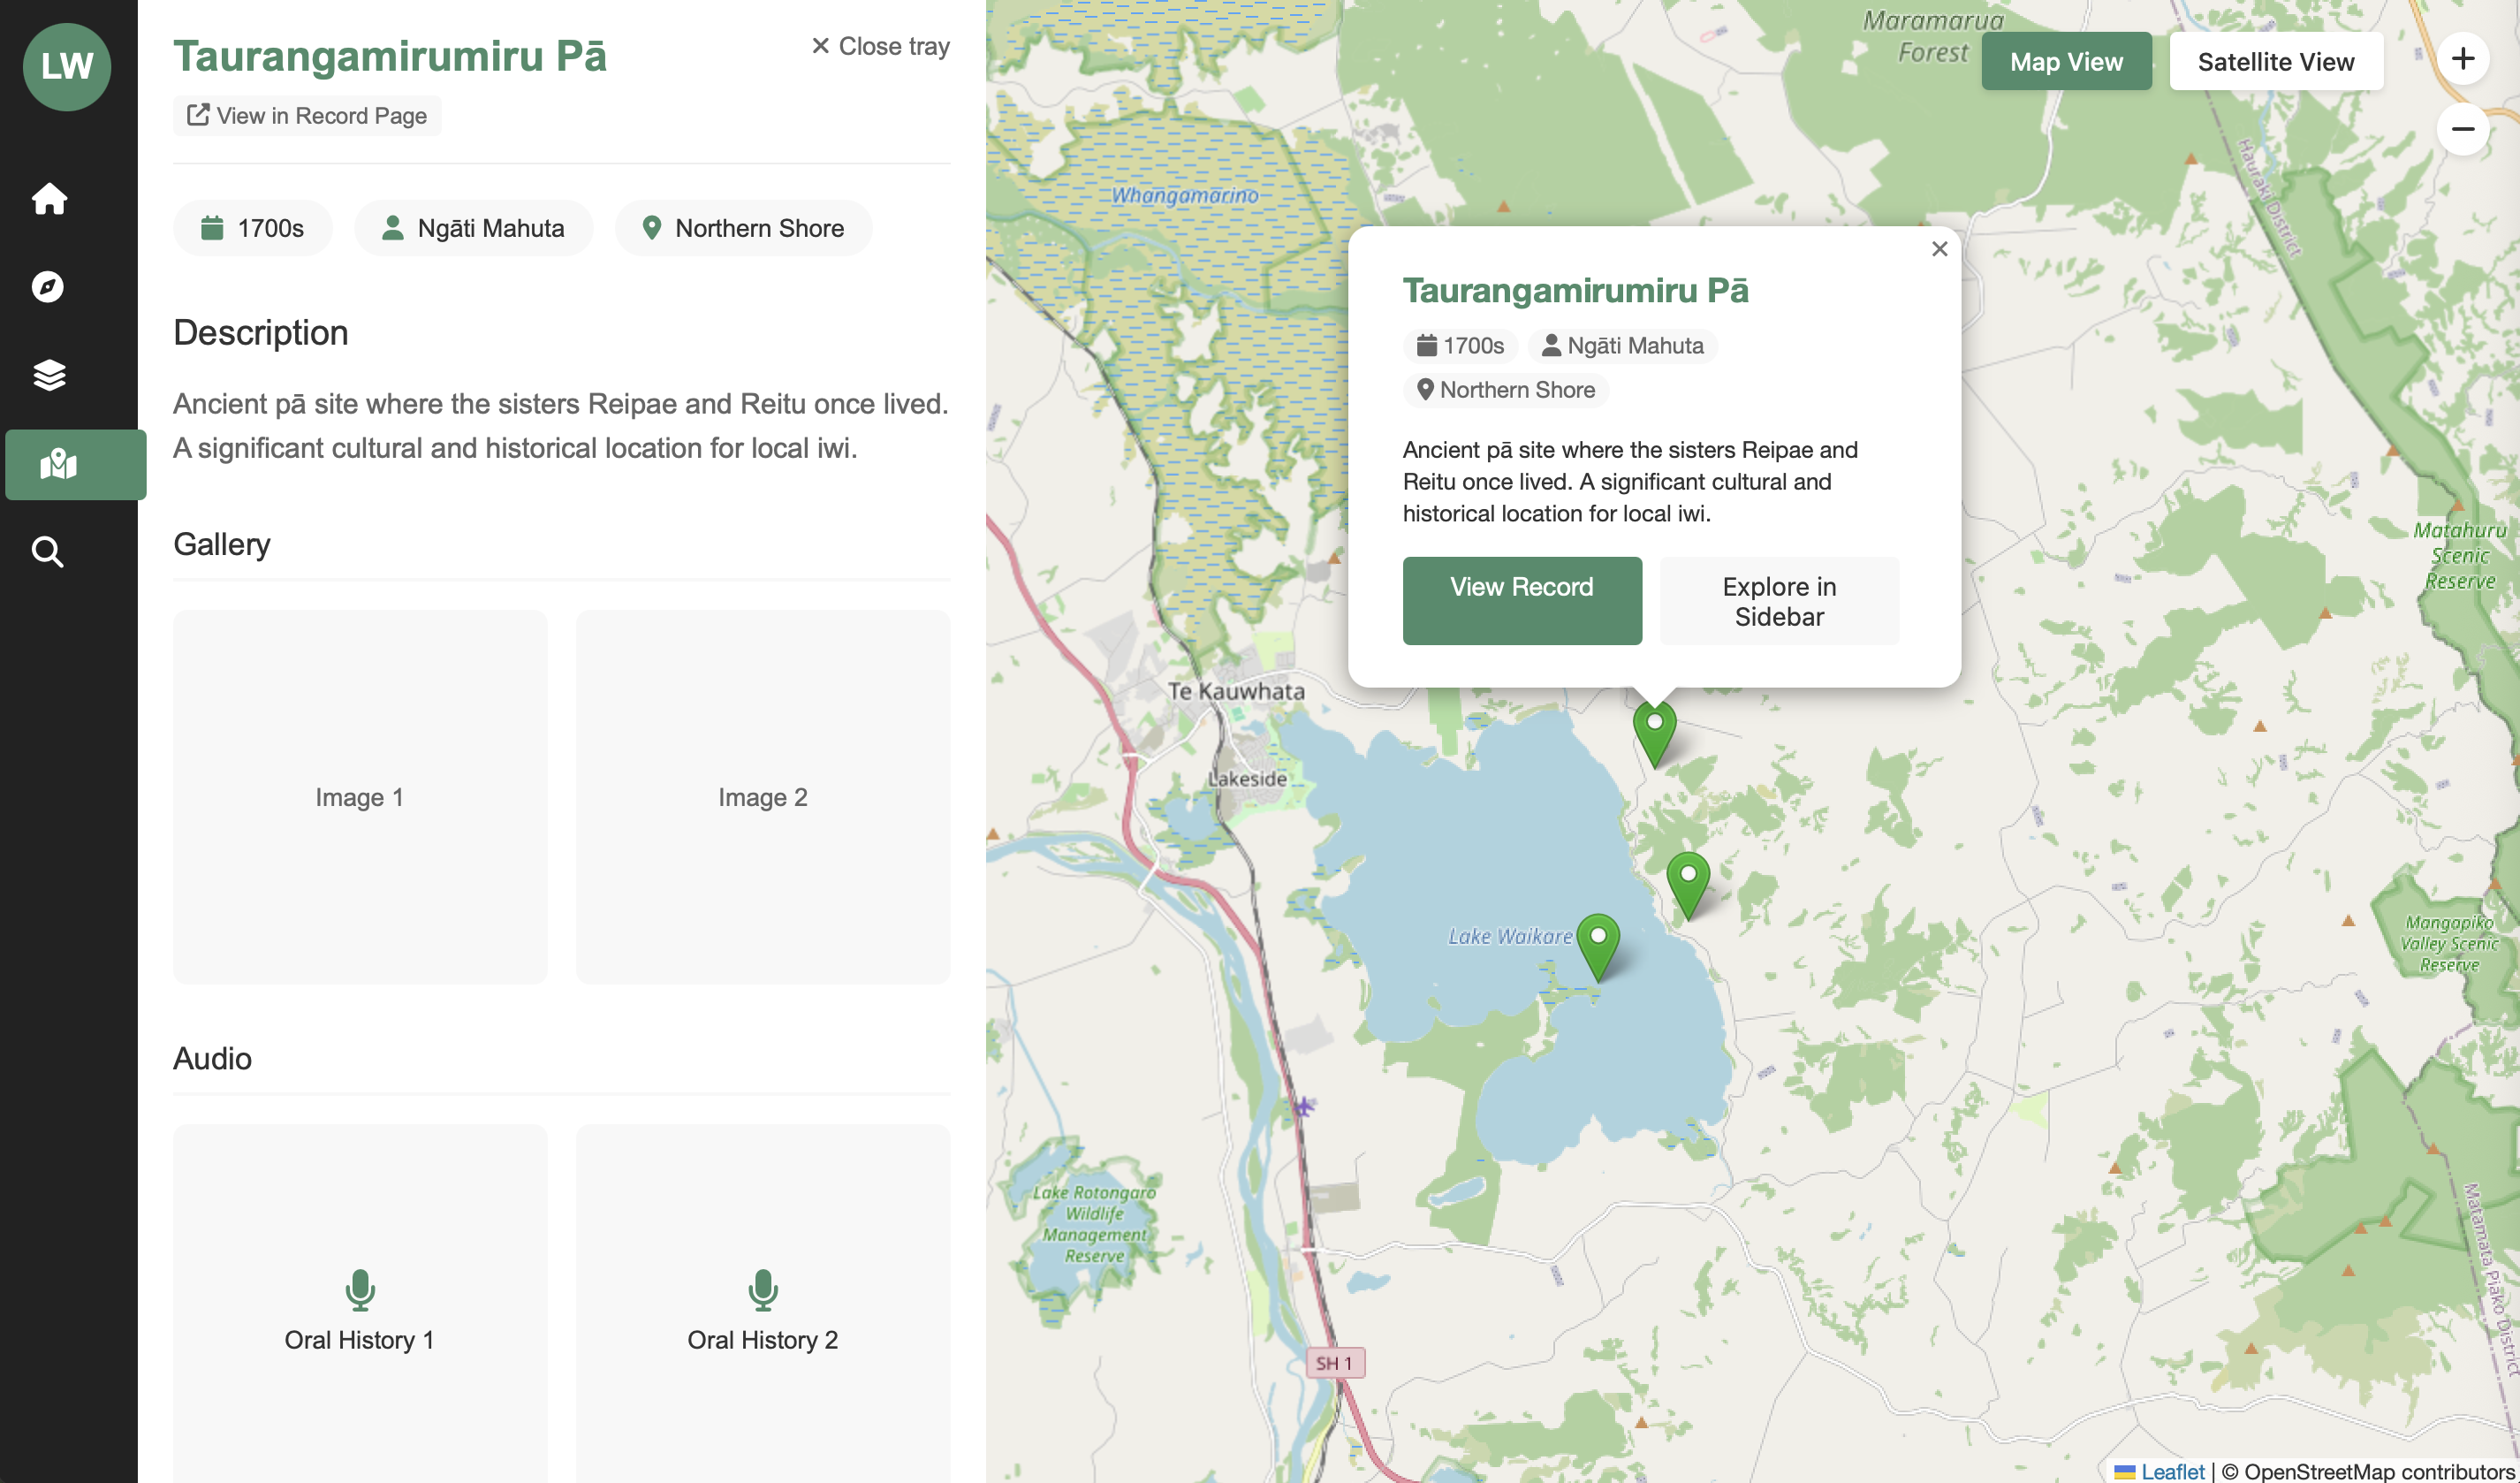
\includegraphics[width=\textwidth]{screenshot/prototype_mapview.png}
    \caption{Map View}
  \end{subfigure}

  \vspace{0.5cm}

  % line 3
  \begin{subfigure}[b]{0.3\textwidth}
    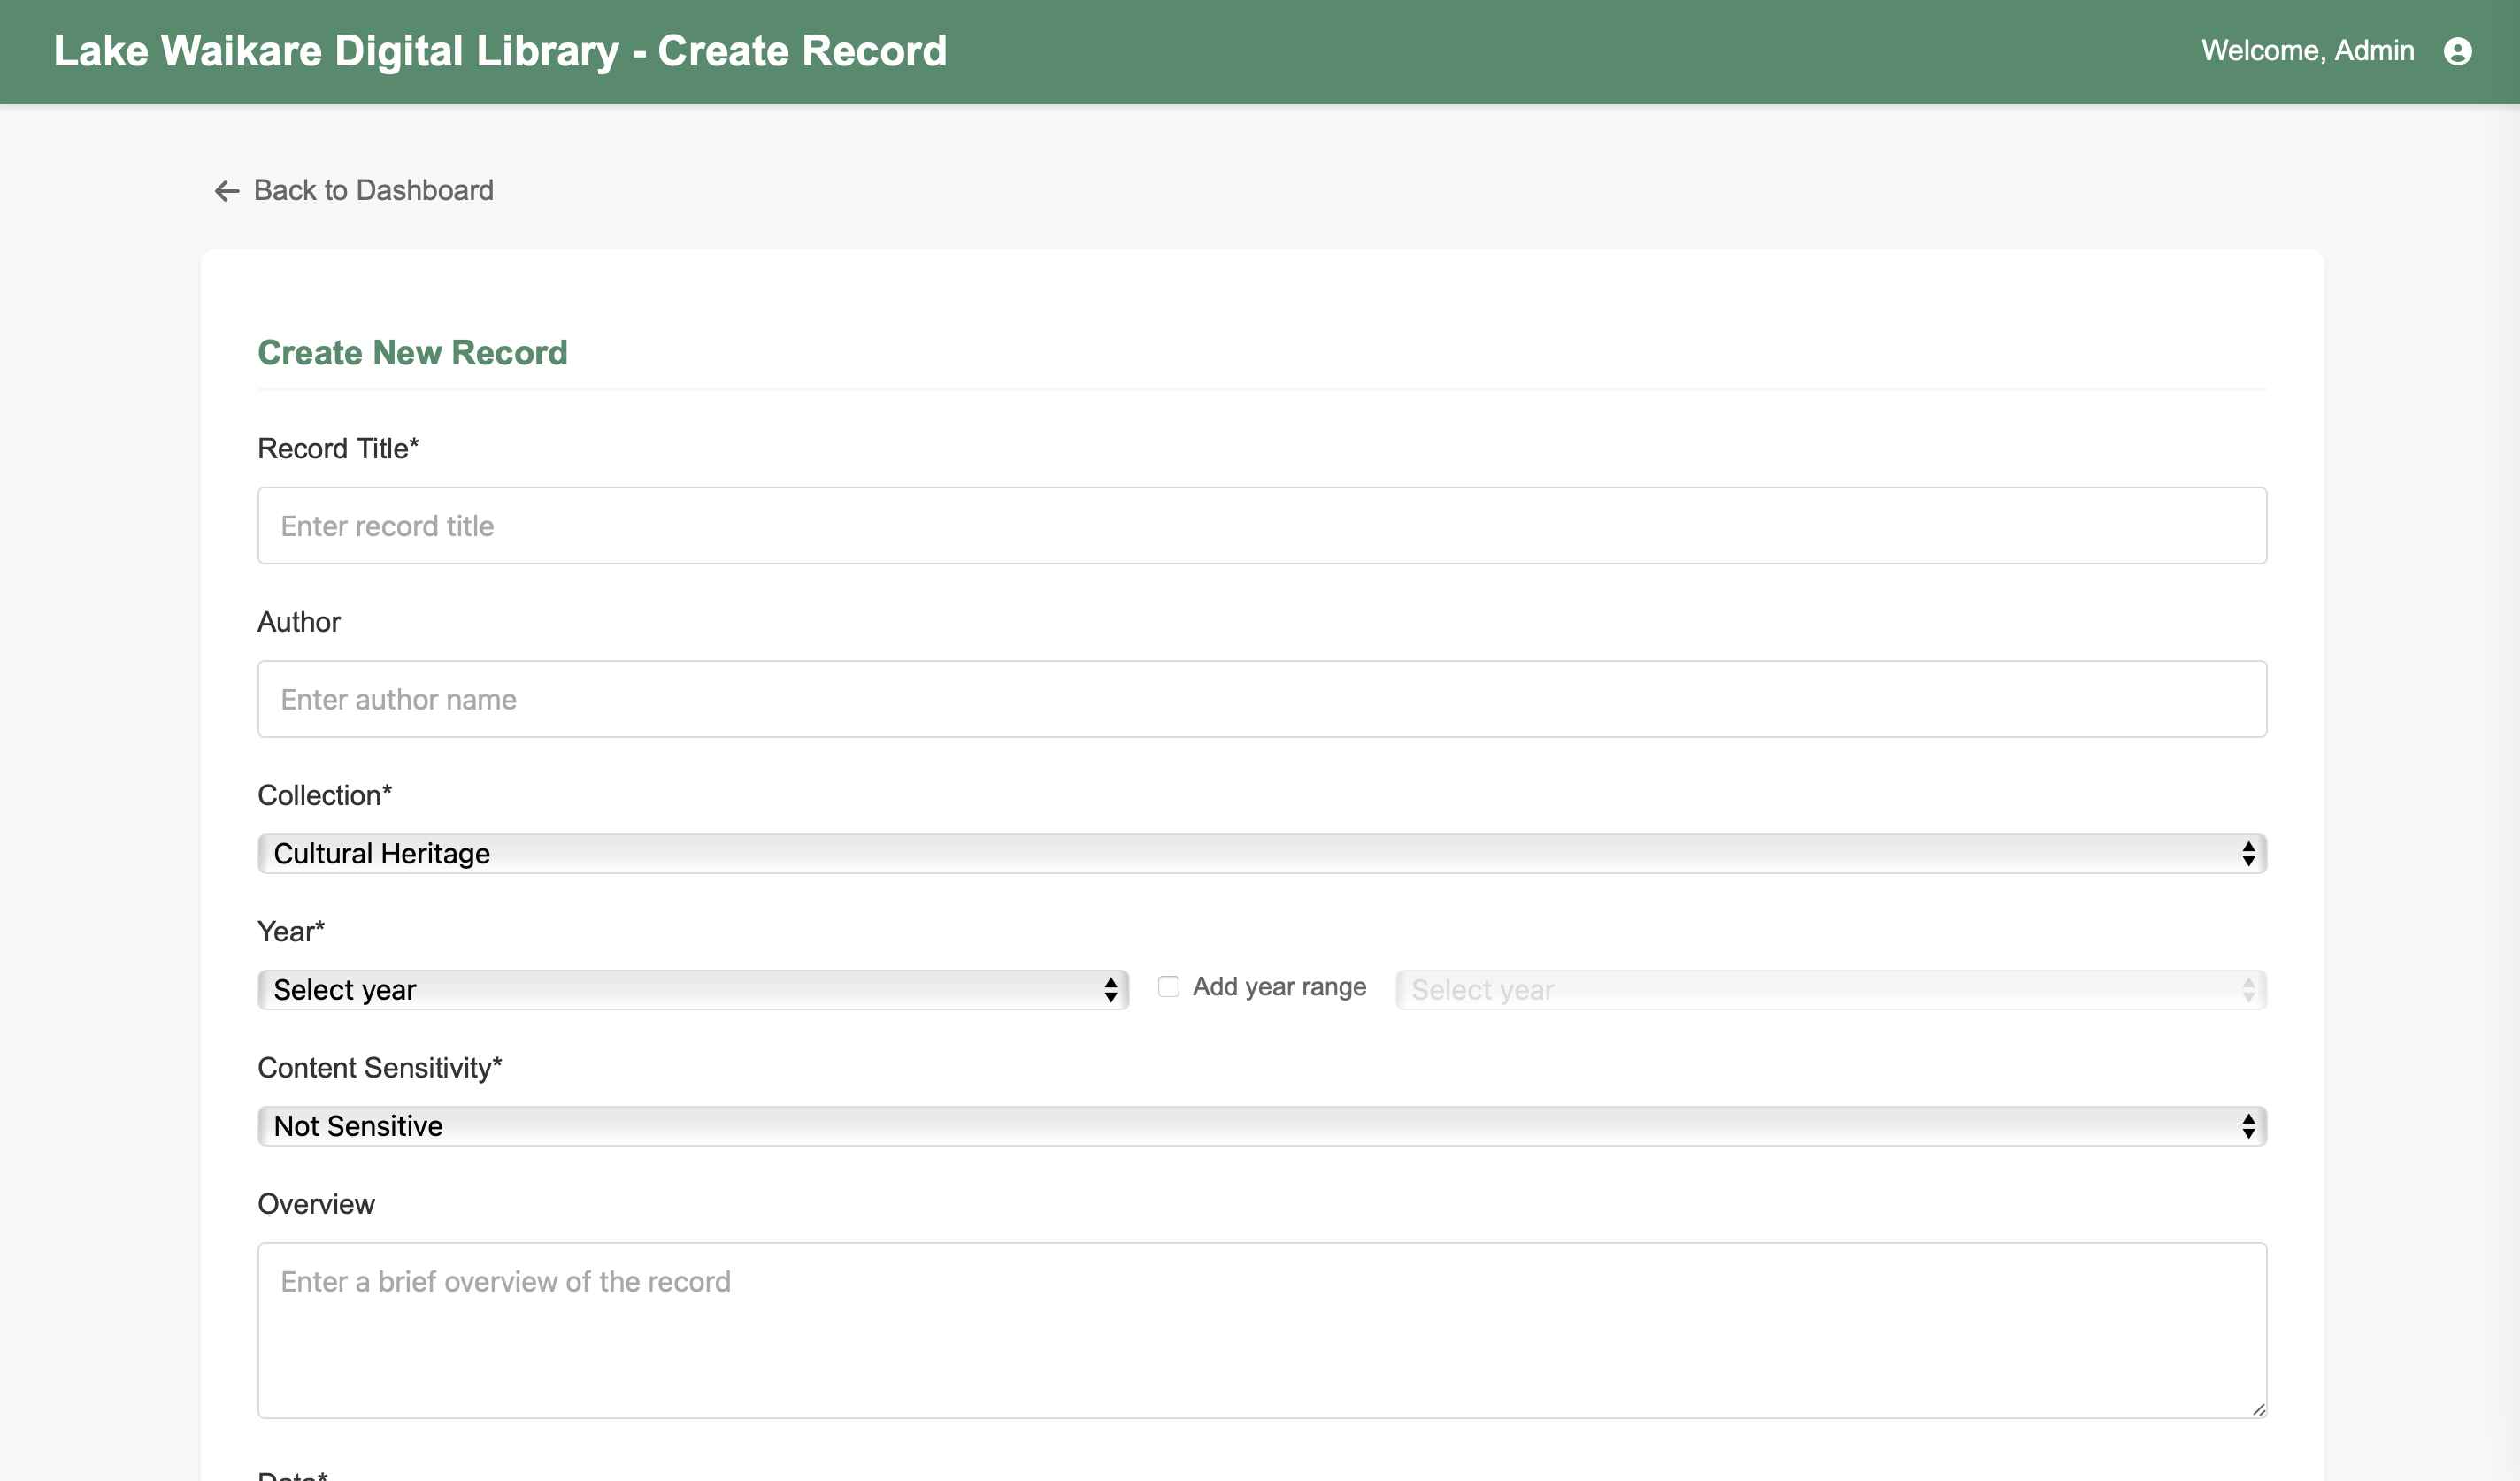
\includegraphics[width=\textwidth]{screenshot/prototype_dashboard_createrecord.png}
    \caption{Dashboard Create Record}
  \end{subfigure}\hfill
  \begin{subfigure}[b]{0.3\textwidth}
    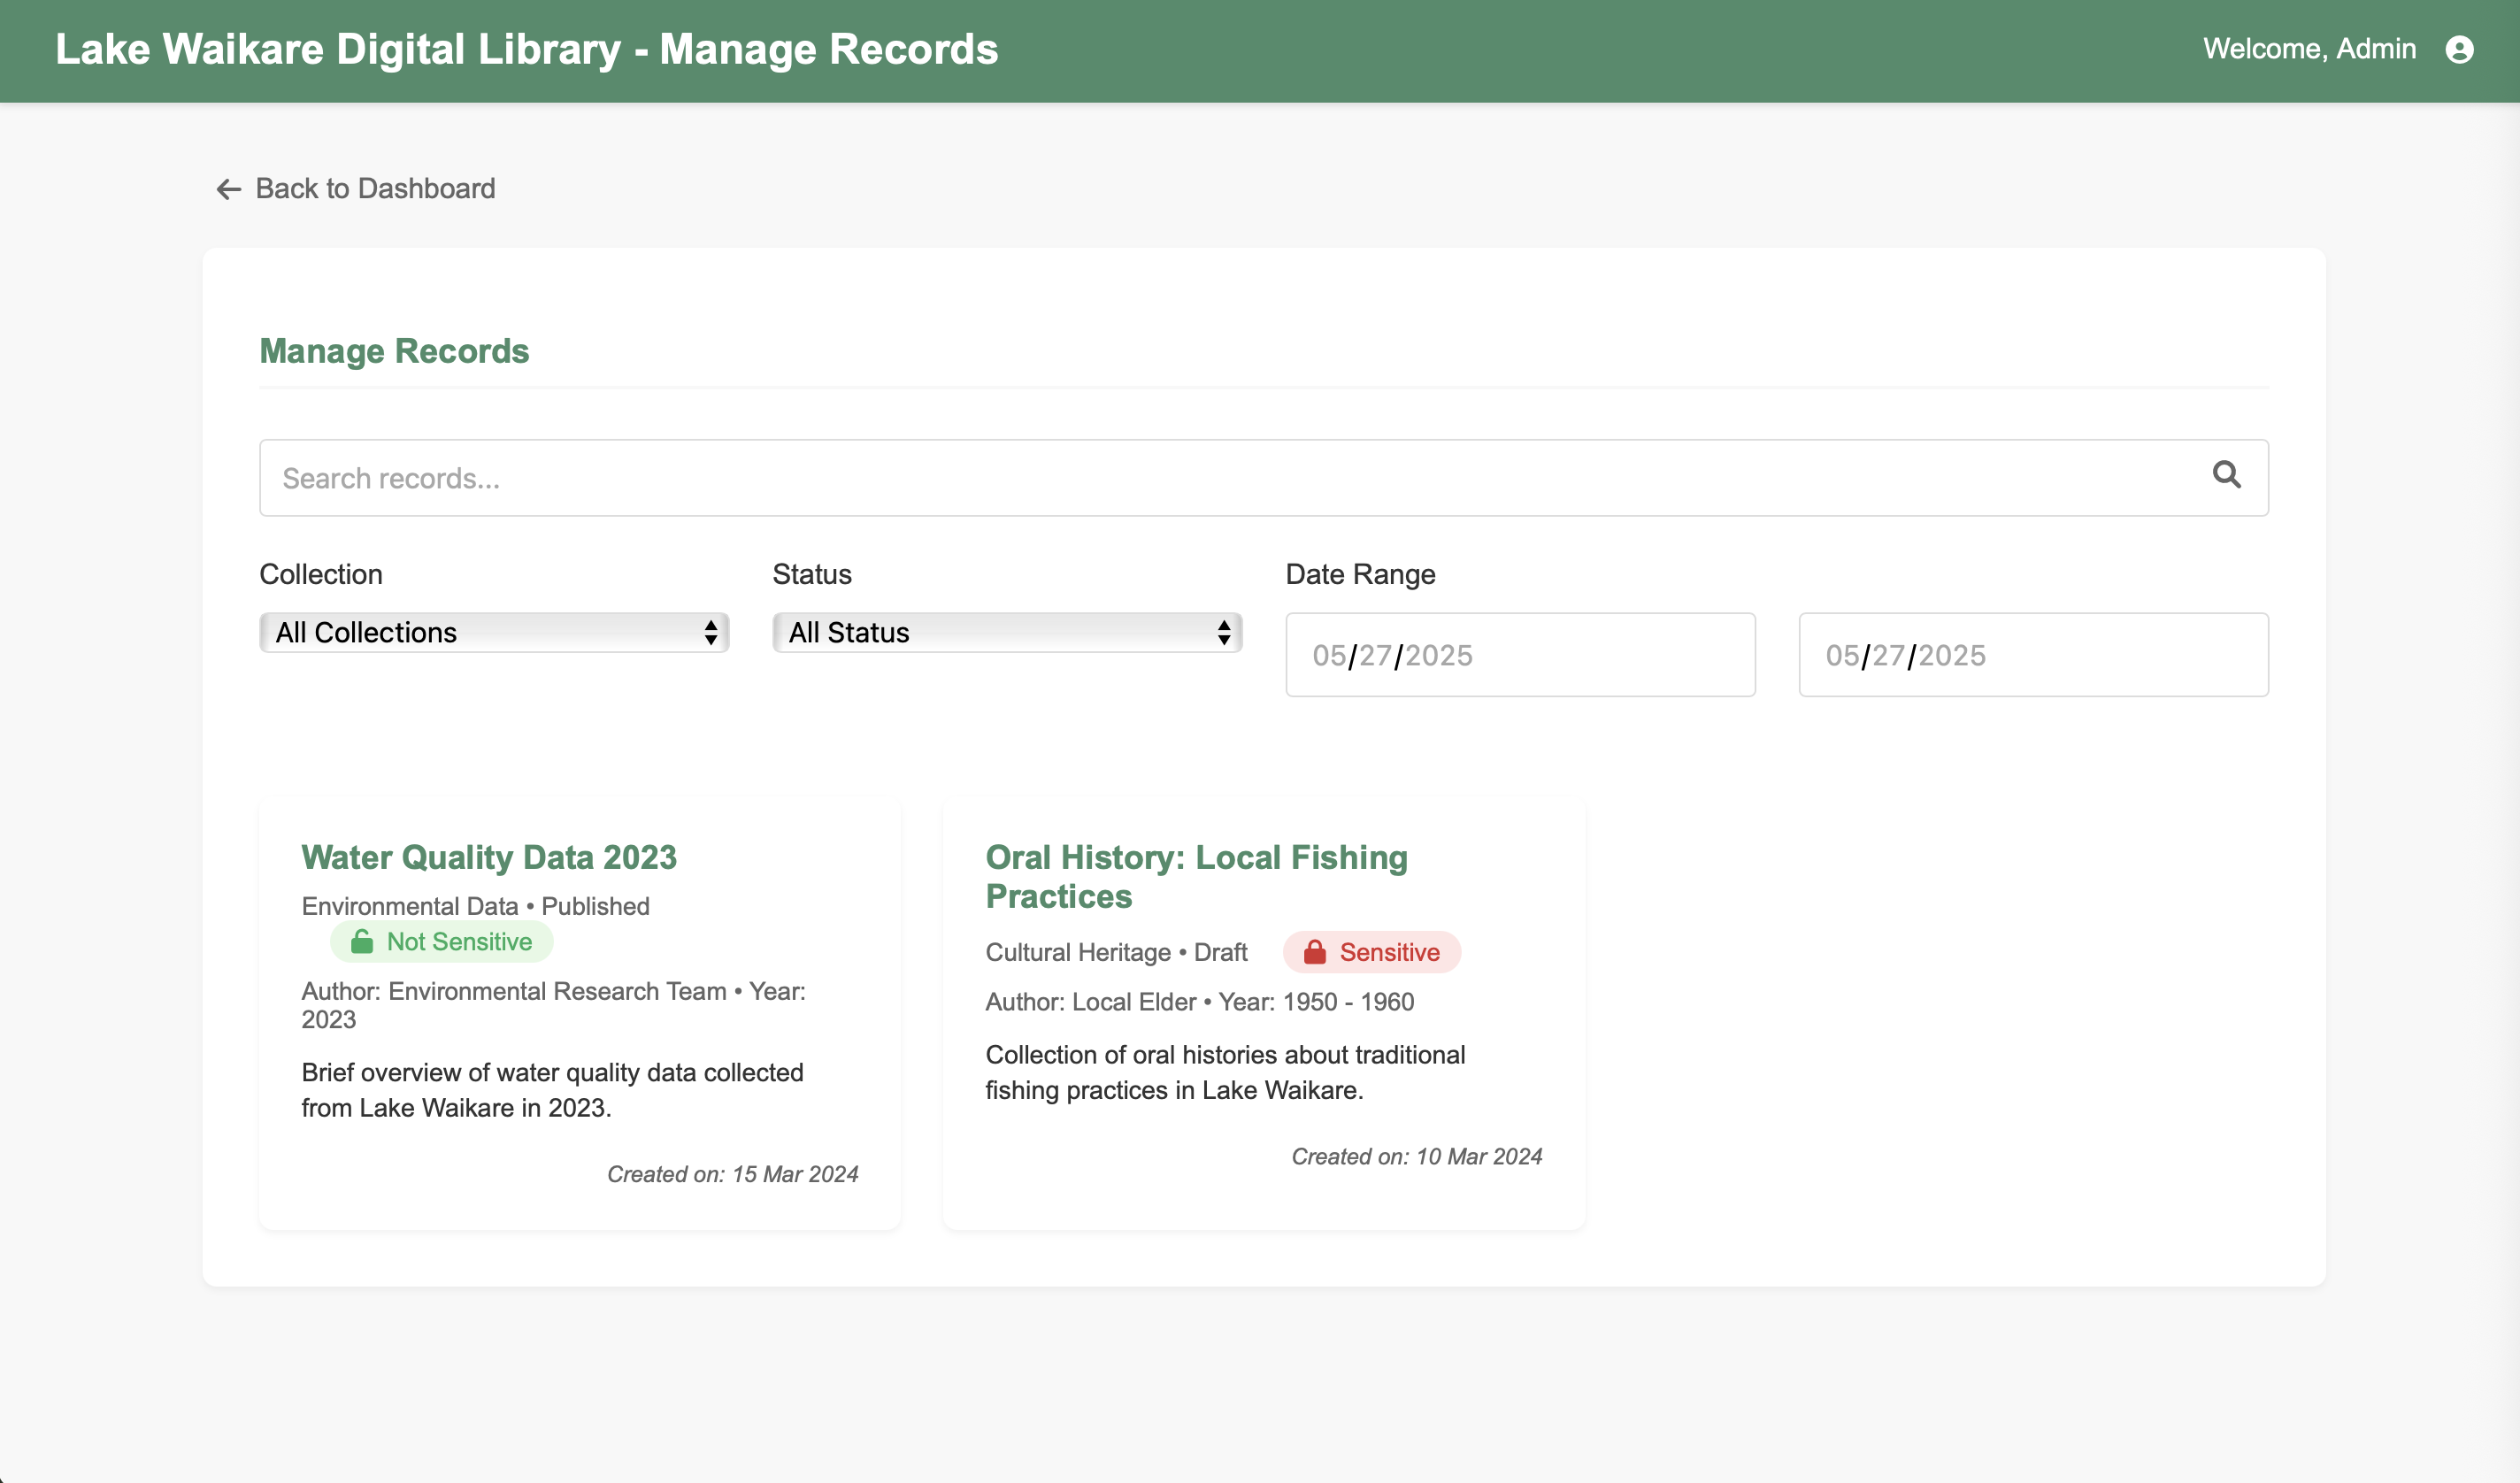
\includegraphics[width=\textwidth]{screenshot/prototype_dashboard_managerecord.png}
    \caption{Dashboard Manage Record}
  \end{subfigure}\hfill
  \begin{subfigure}[b]{0.3\textwidth}
    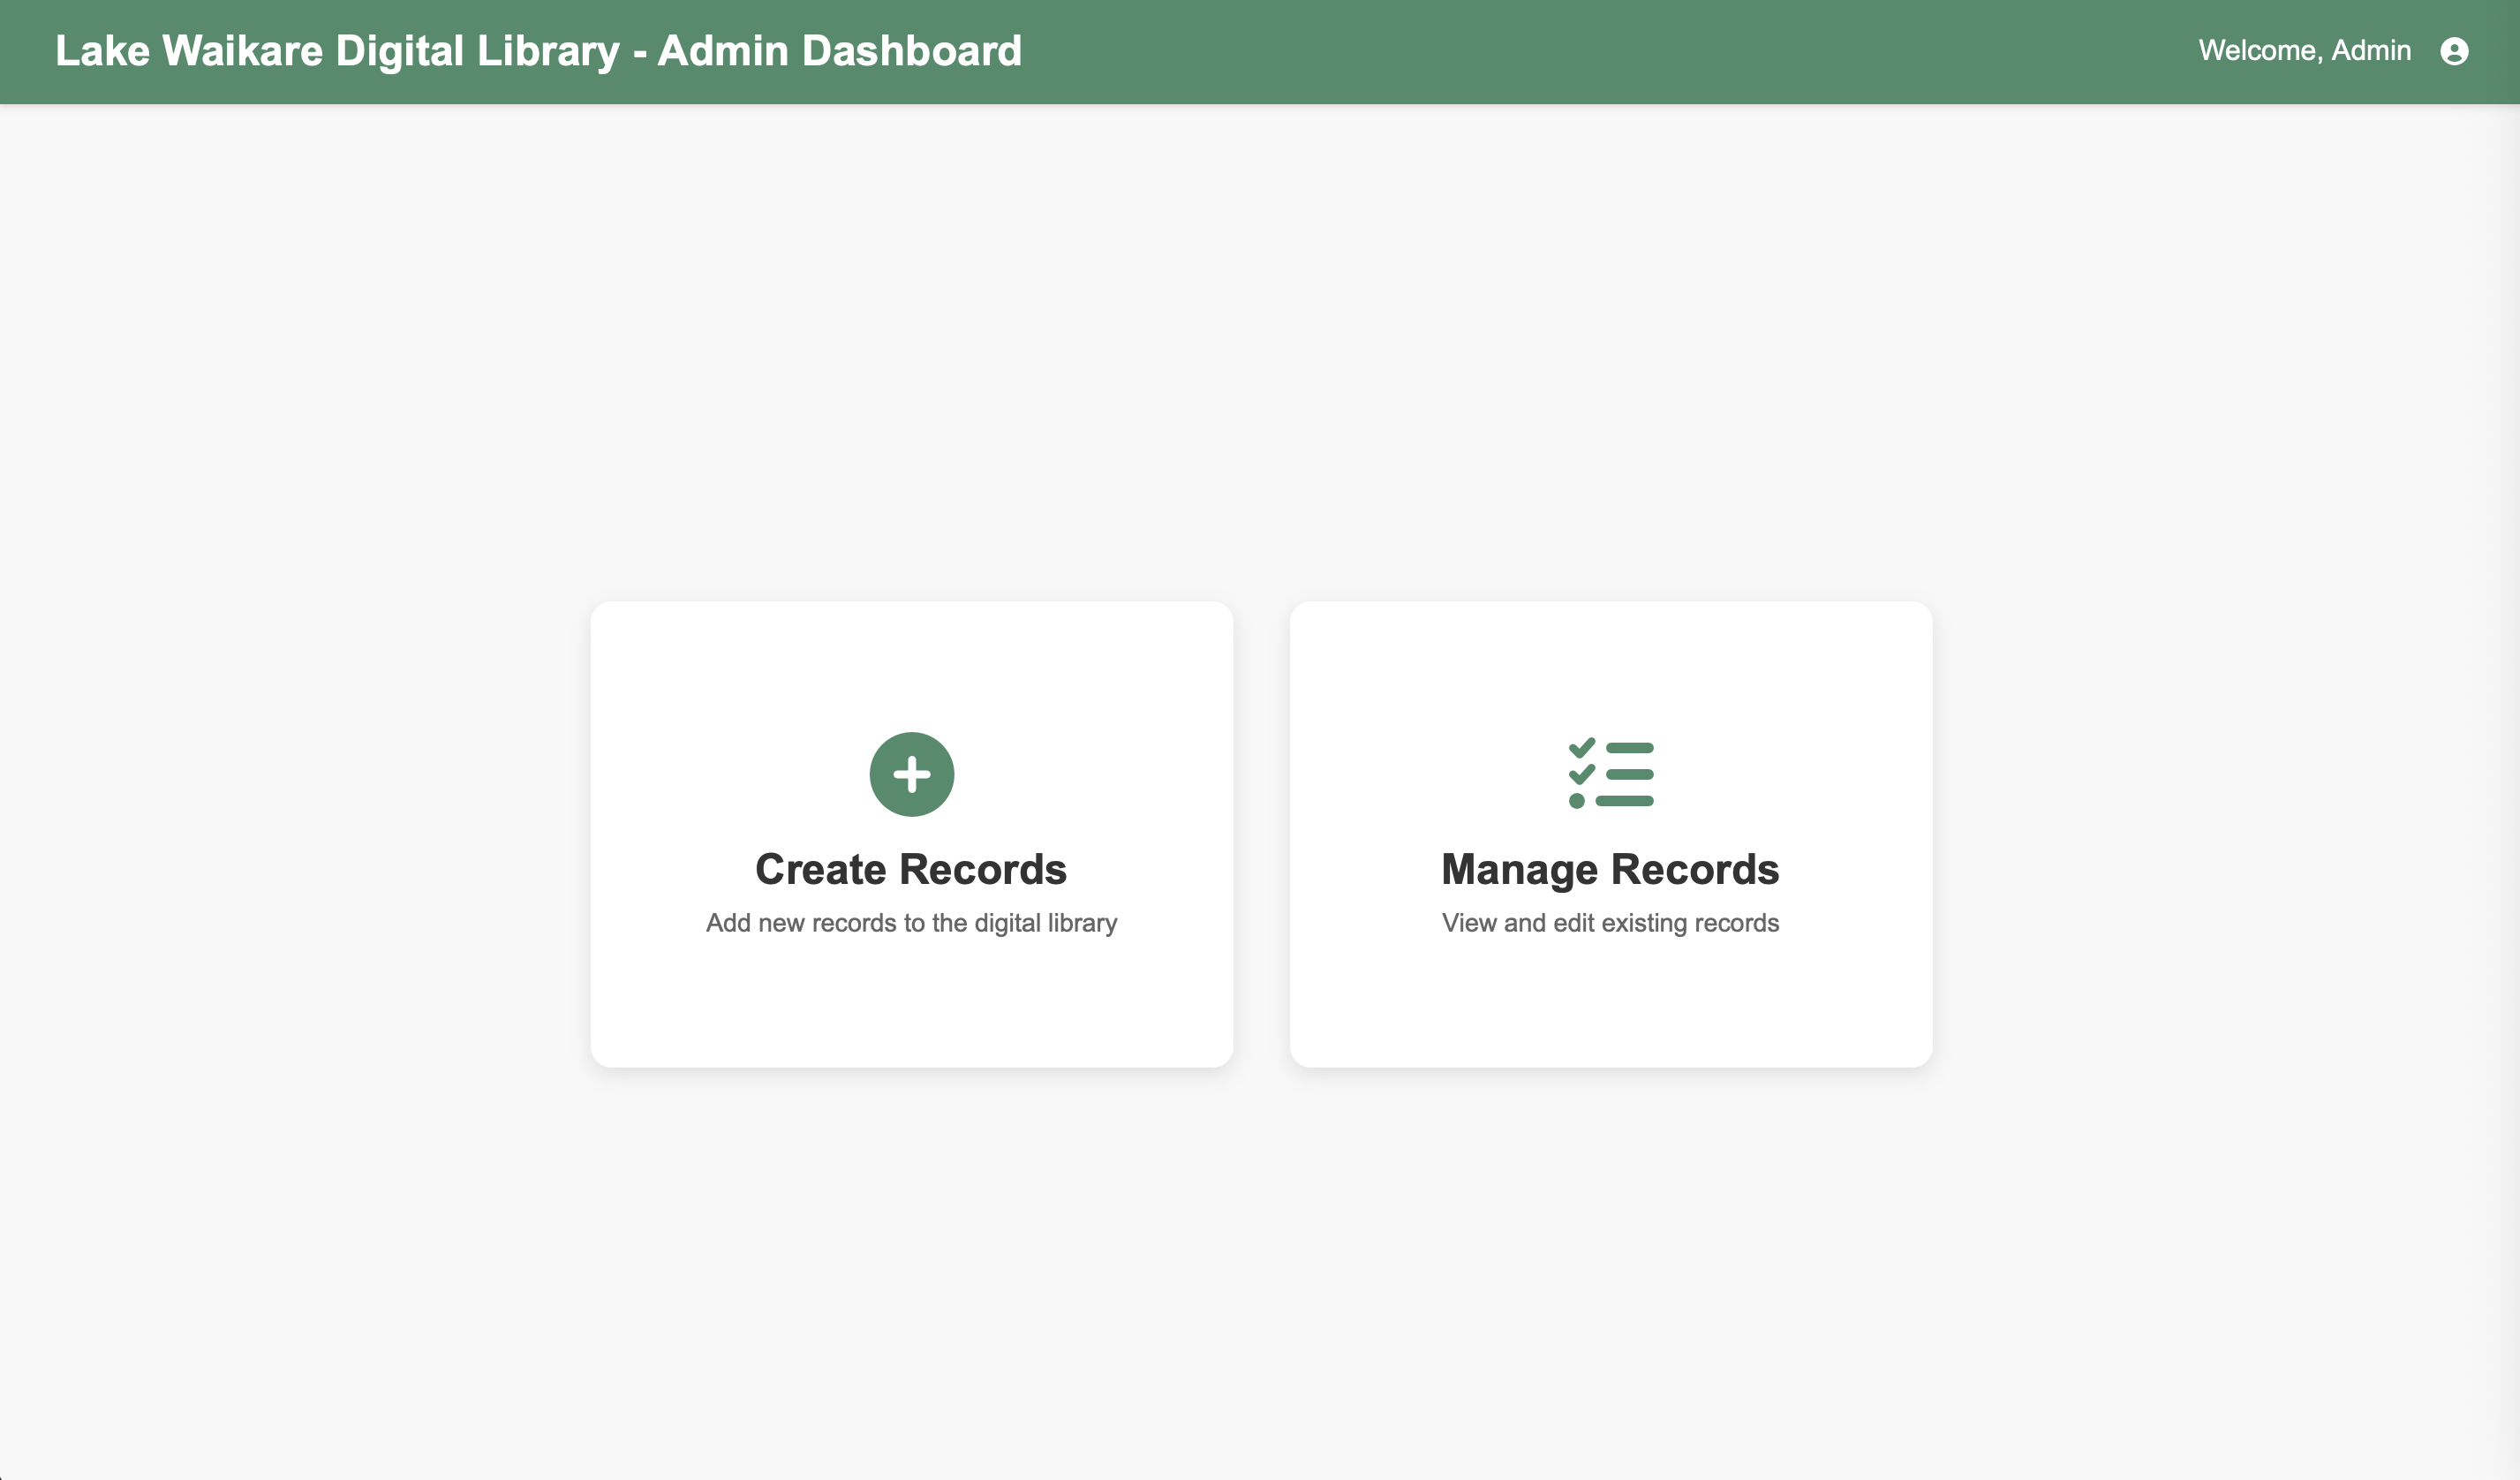
\includegraphics[width=\textwidth]{screenshot/prototype_dashboard.png}
    \caption{Dashboard}
  \end{subfigure}

  \vspace{0.5cm}

  % line 4
  \begin{subfigure}[b]{0.3\textwidth}
    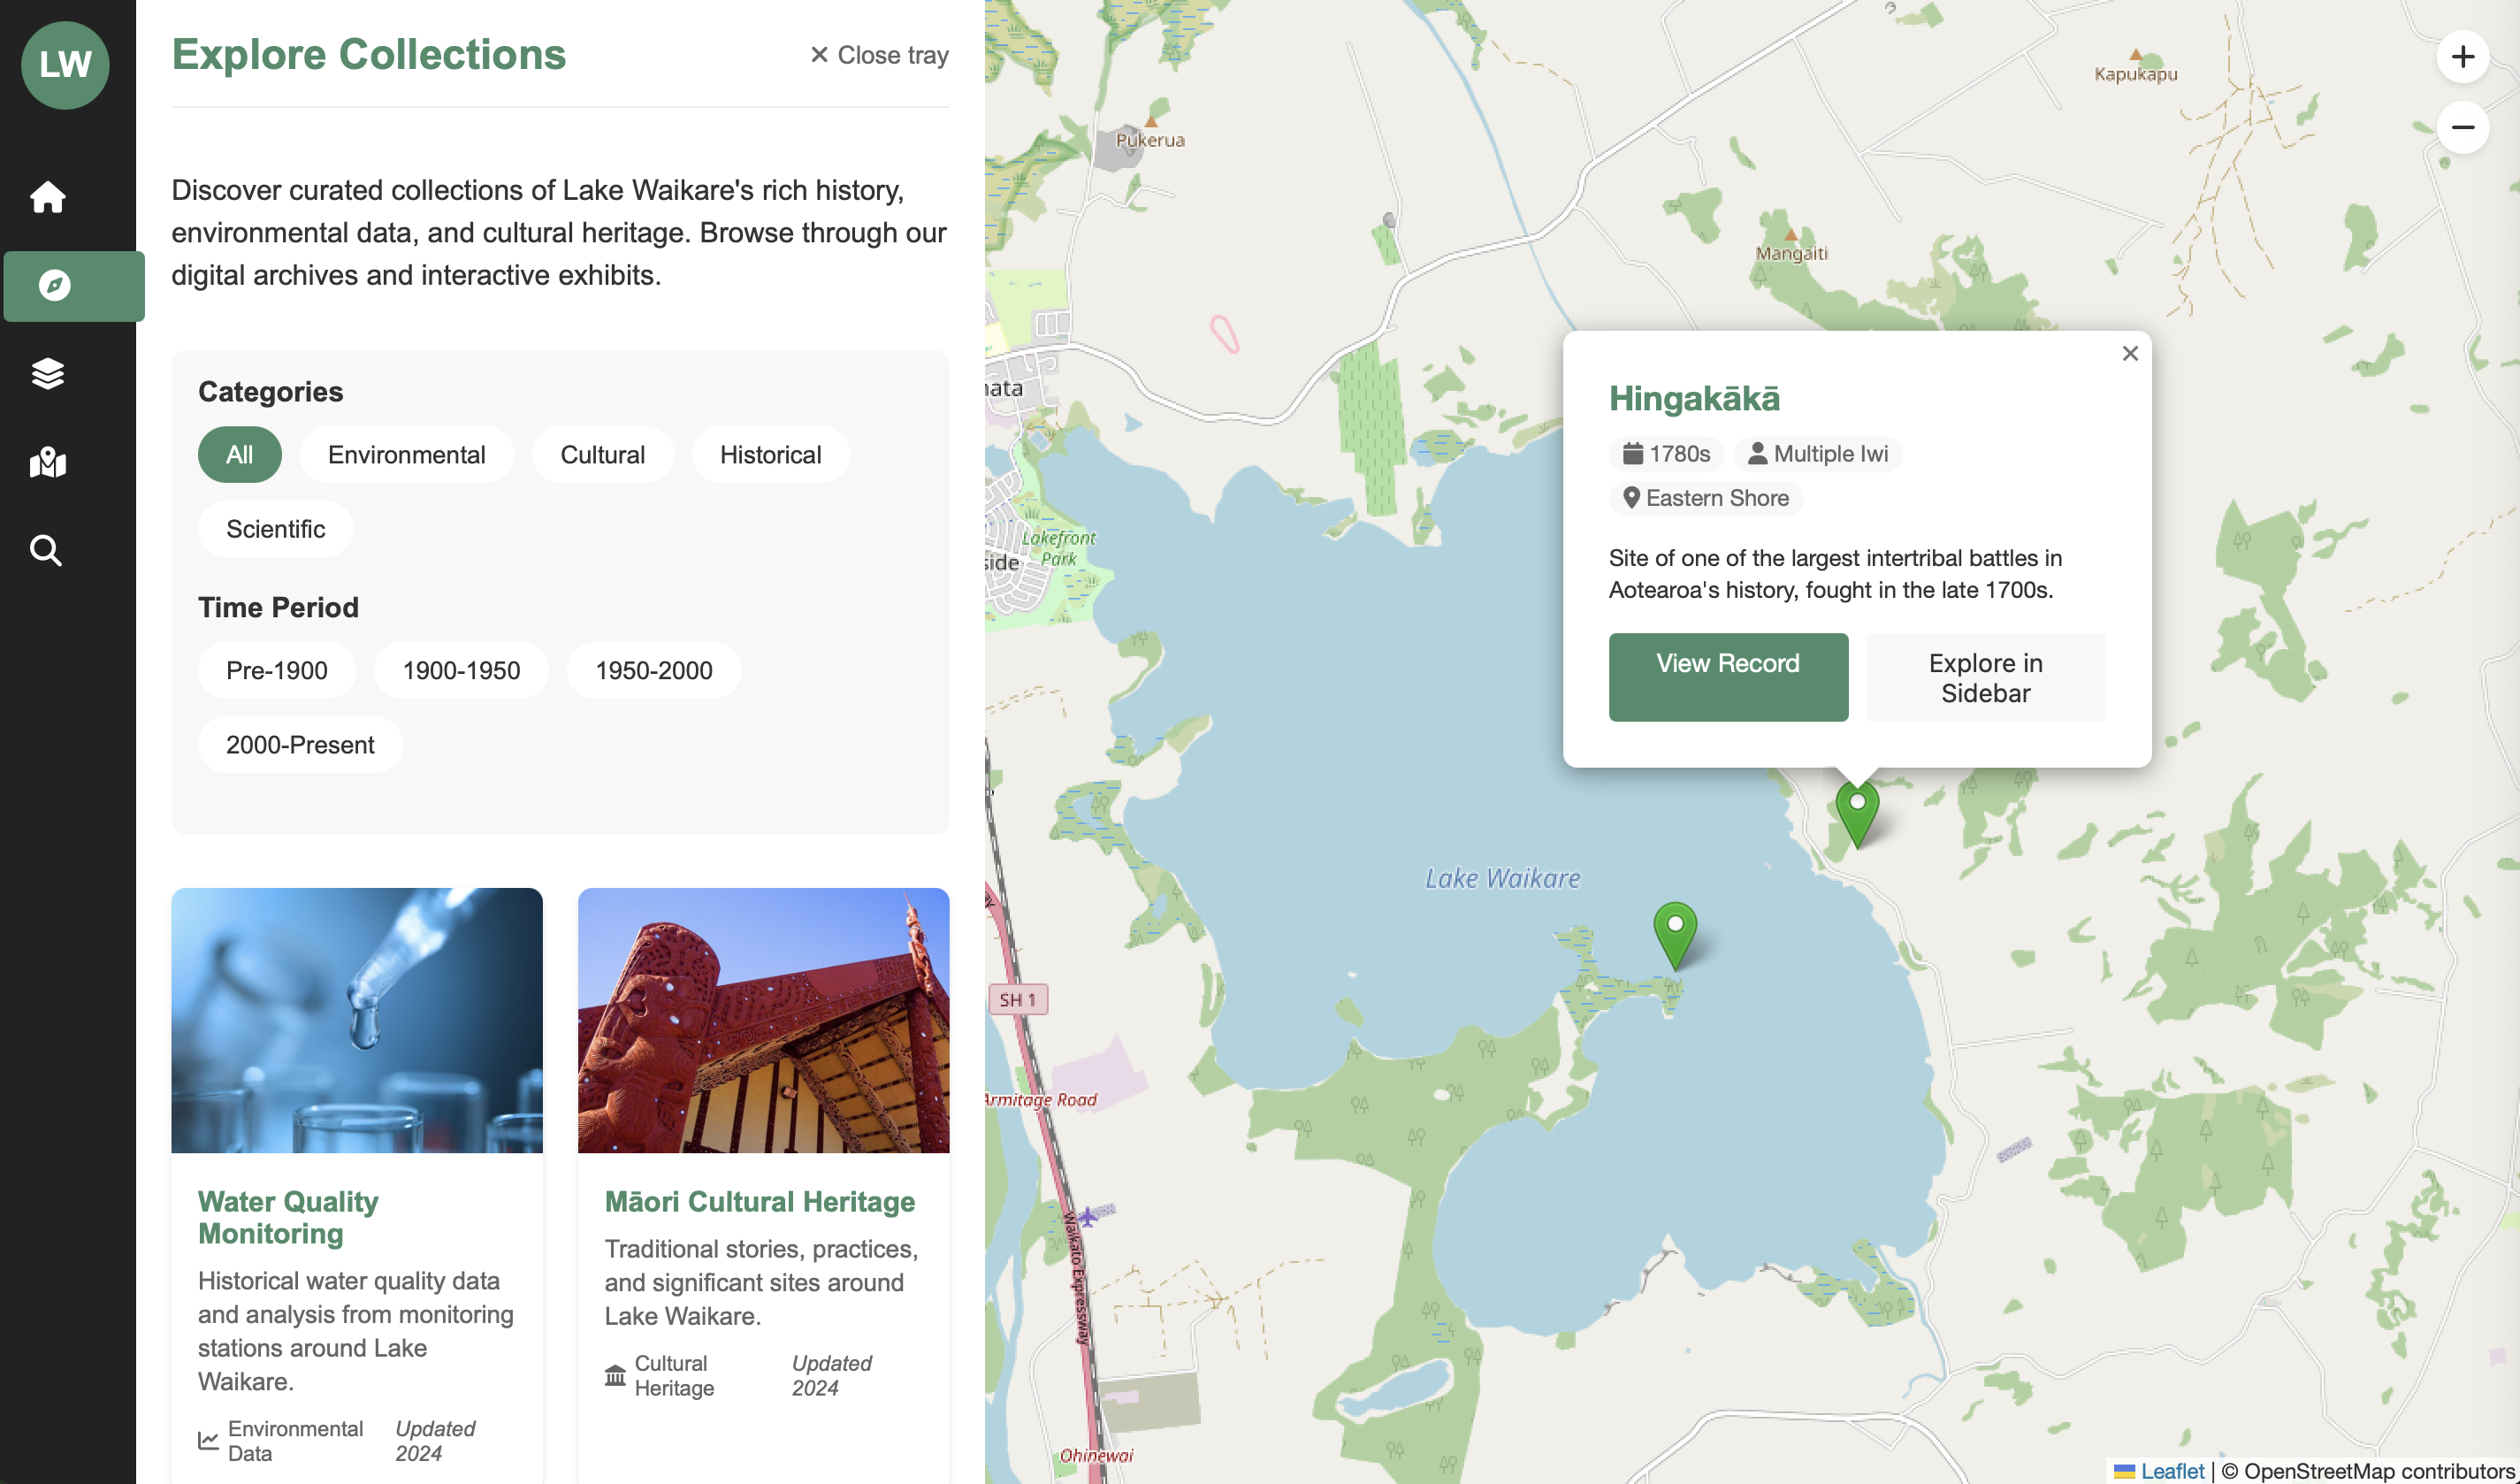
\includegraphics[width=\textwidth]{screenshot/prototype_explore.png}
    \caption{Explore}
  \end{subfigure}\hfill
  \begin{subfigure}[b]{0.3\textwidth}
    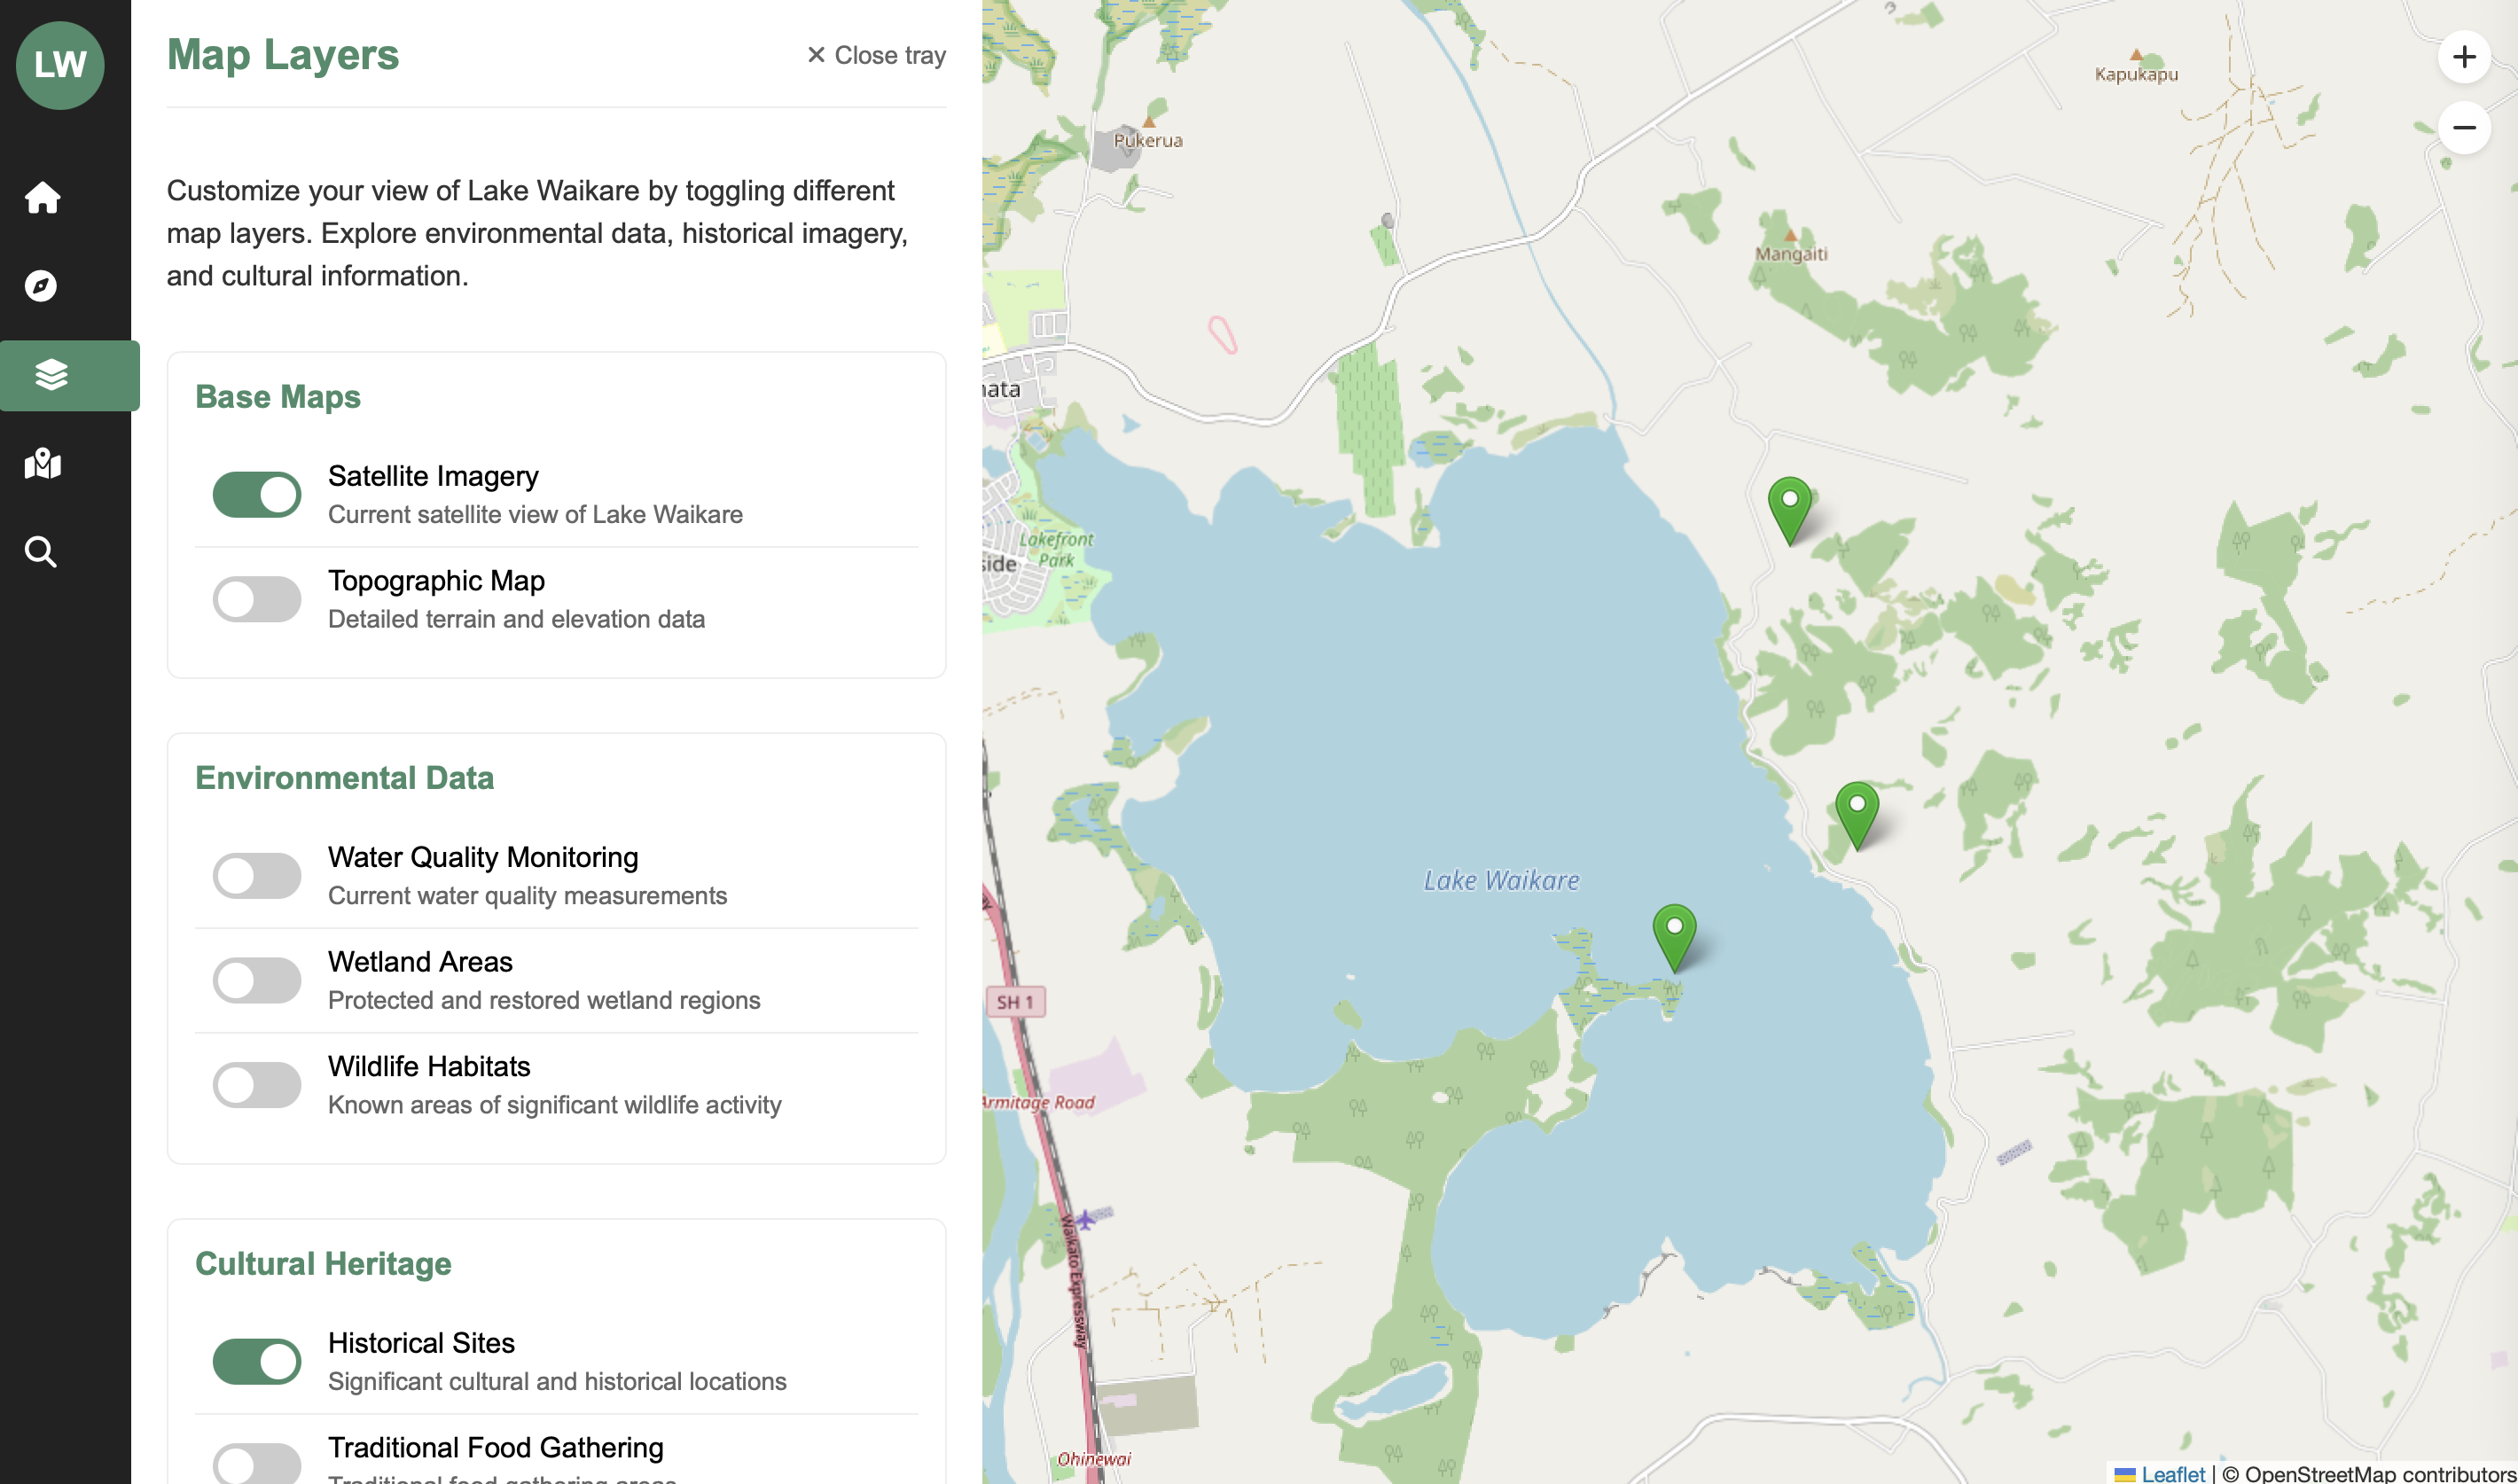
\includegraphics[width=\textwidth]{screenshot/prototype_overlay.png}
    \caption{Overlay}
  \end{subfigure}\hfill
  \begin{subfigure}[b]{0.3\textwidth}
    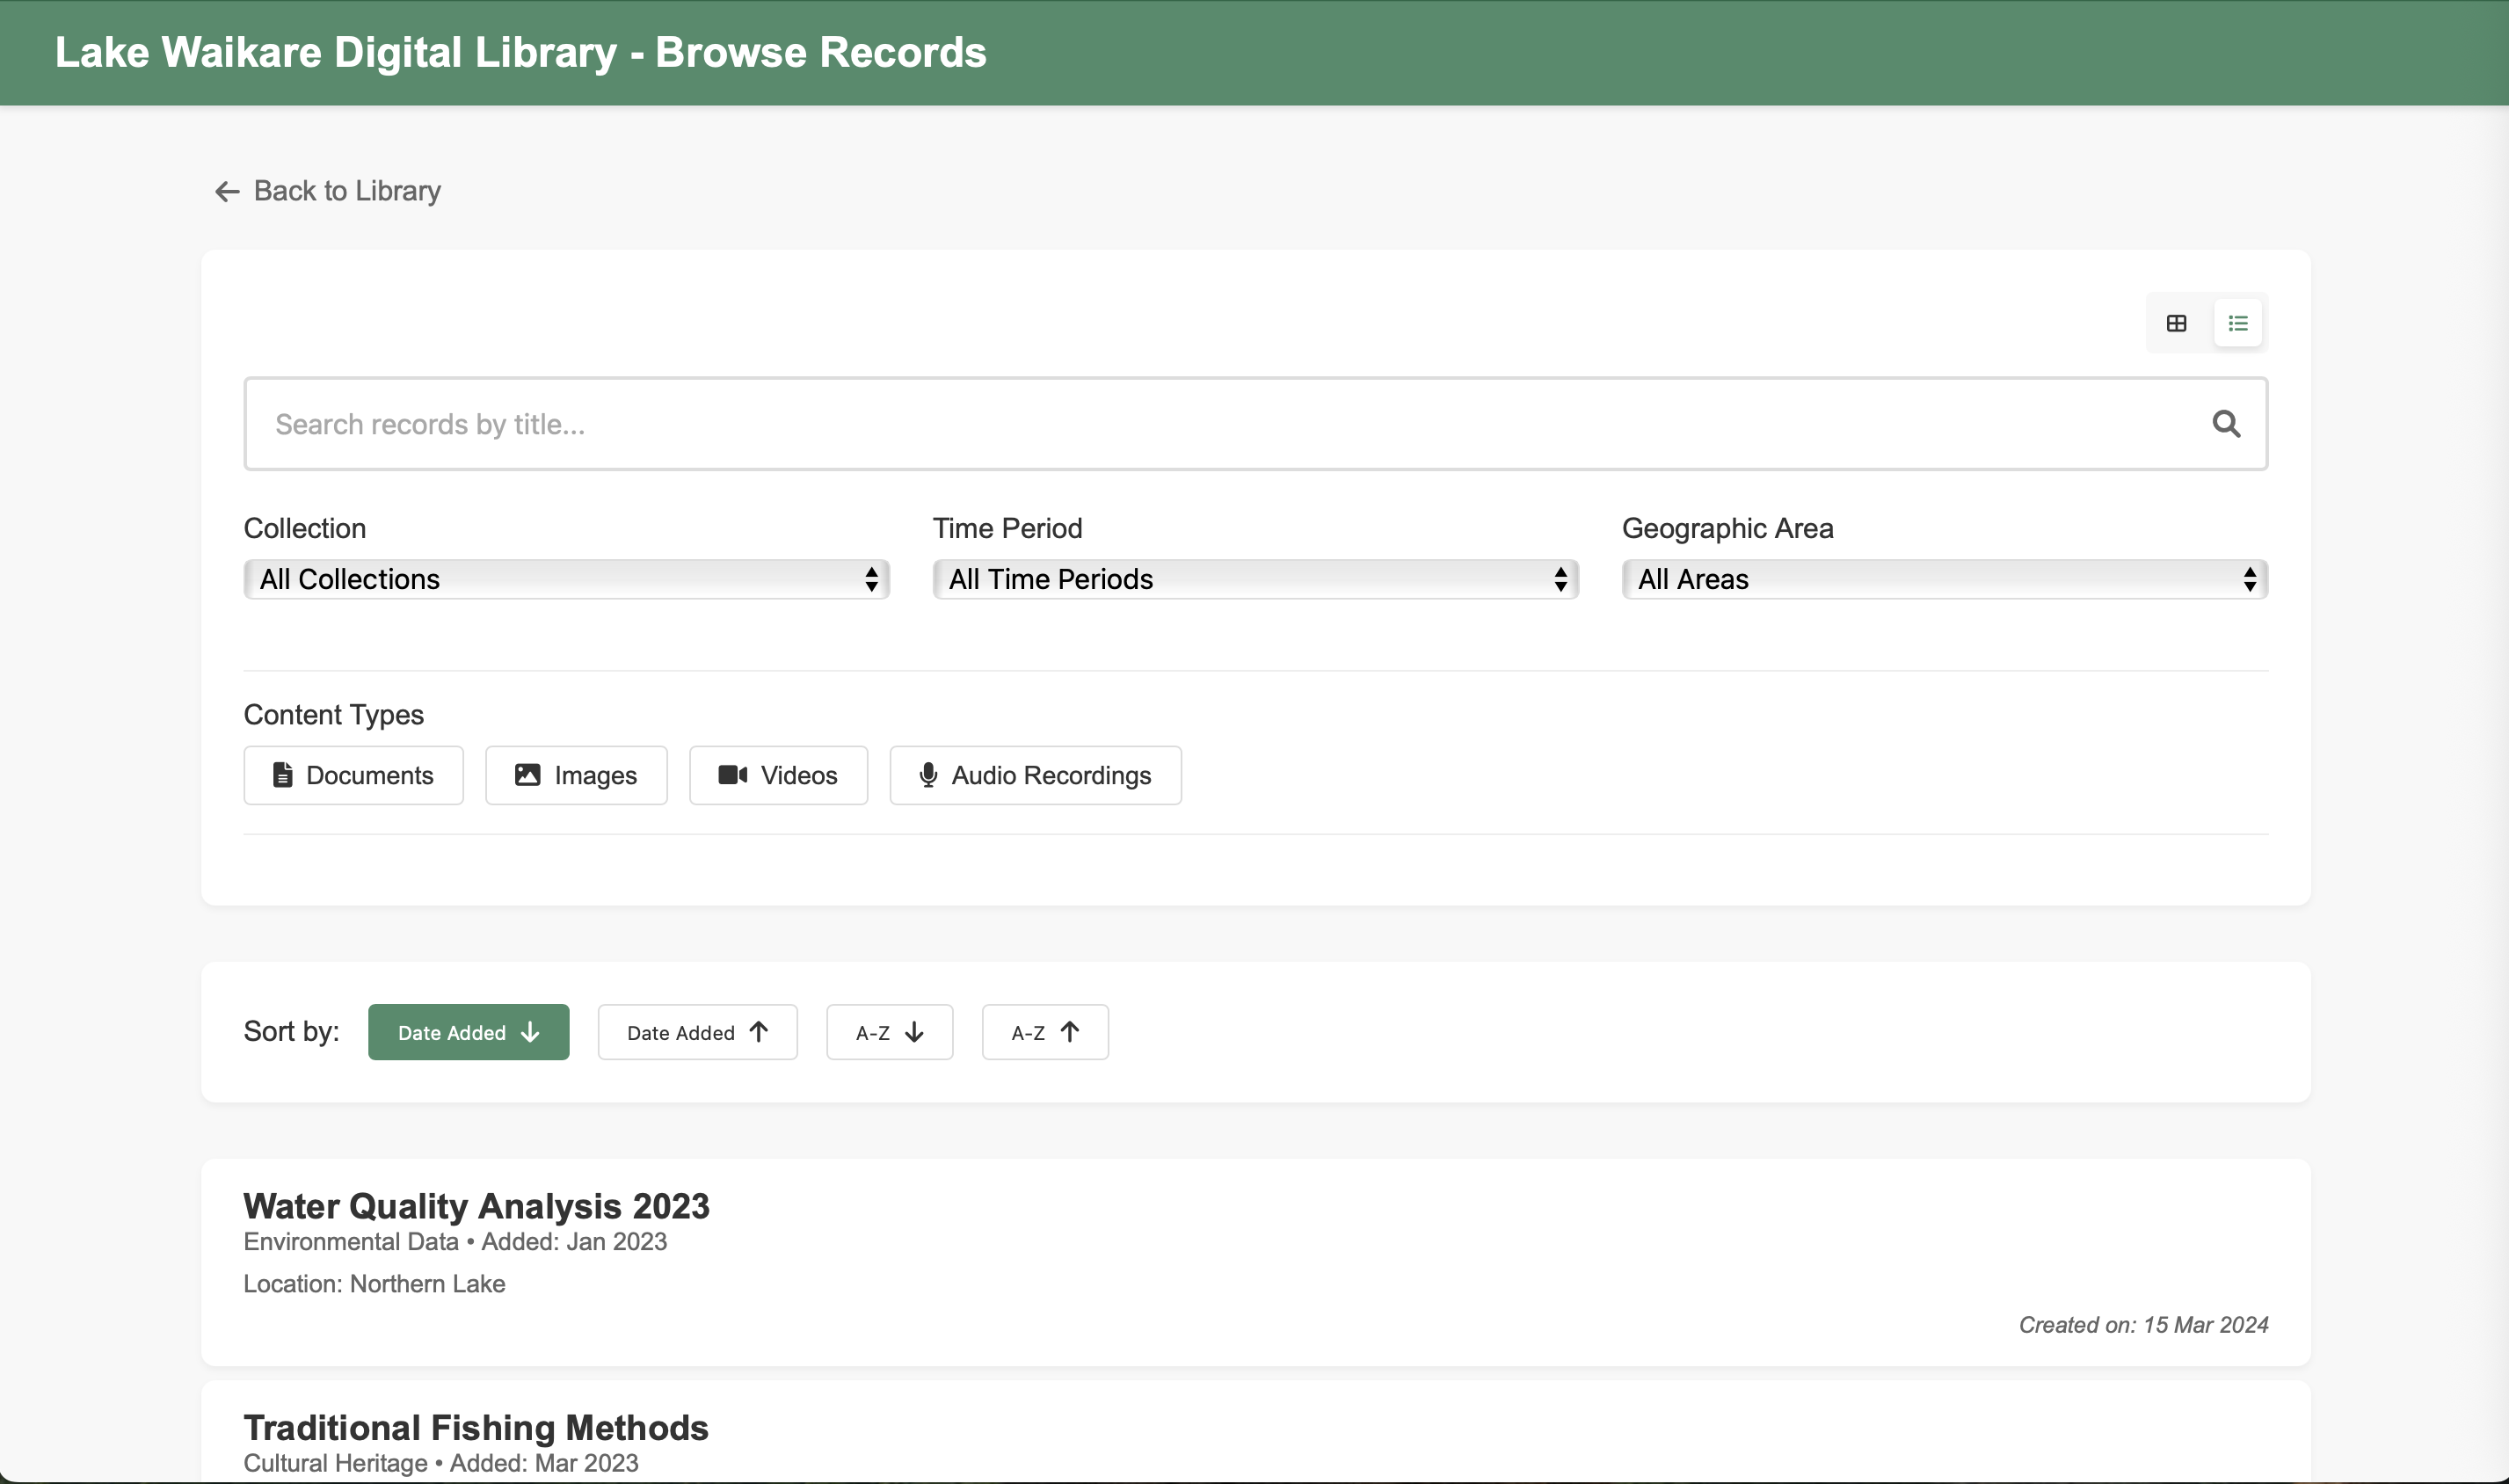
\includegraphics[width=\textwidth]{screenshot/prototype_records.png}
    \caption{Records}
  \end{subfigure}

  \vspace{0.5cm}

  % line 5
  \begin{subfigure}[b]{0.3\textwidth}
    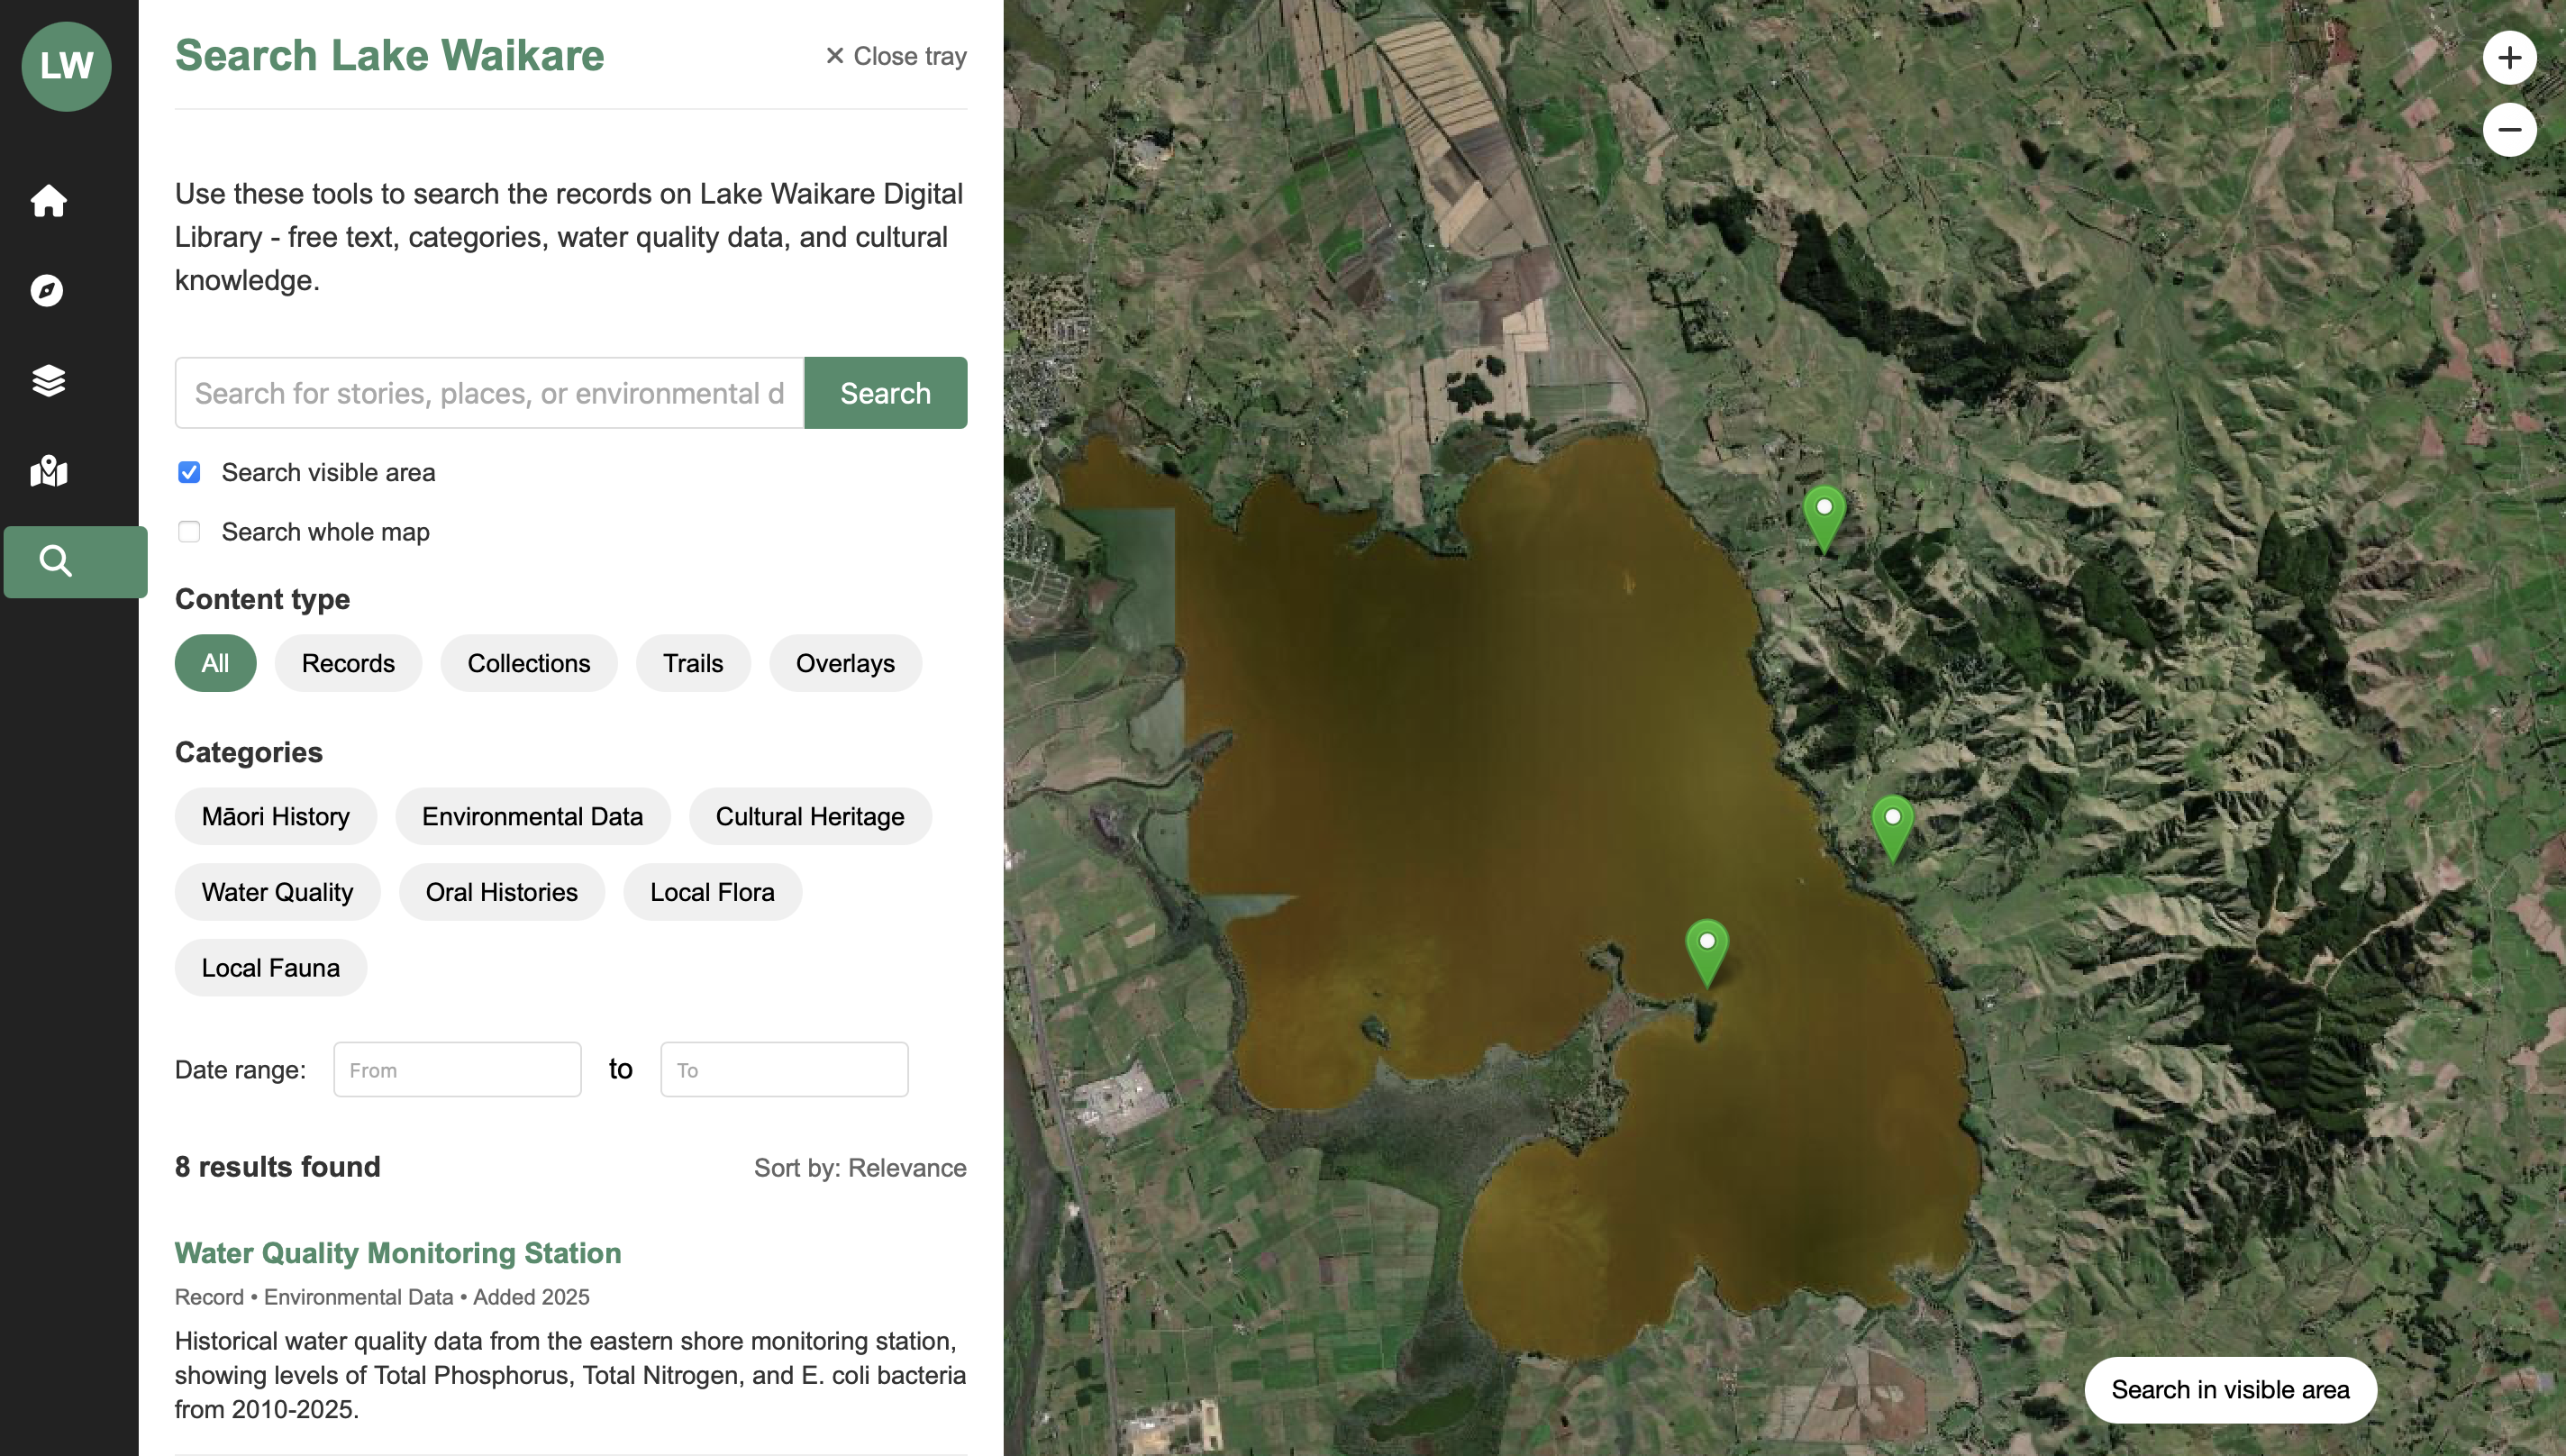
\includegraphics[width=\textwidth]{screenshot/prototype_search.png}
    \caption{Search}
  \end{subfigure}\hfill
  \begin{subfigure}[b]{0.3\textwidth}
    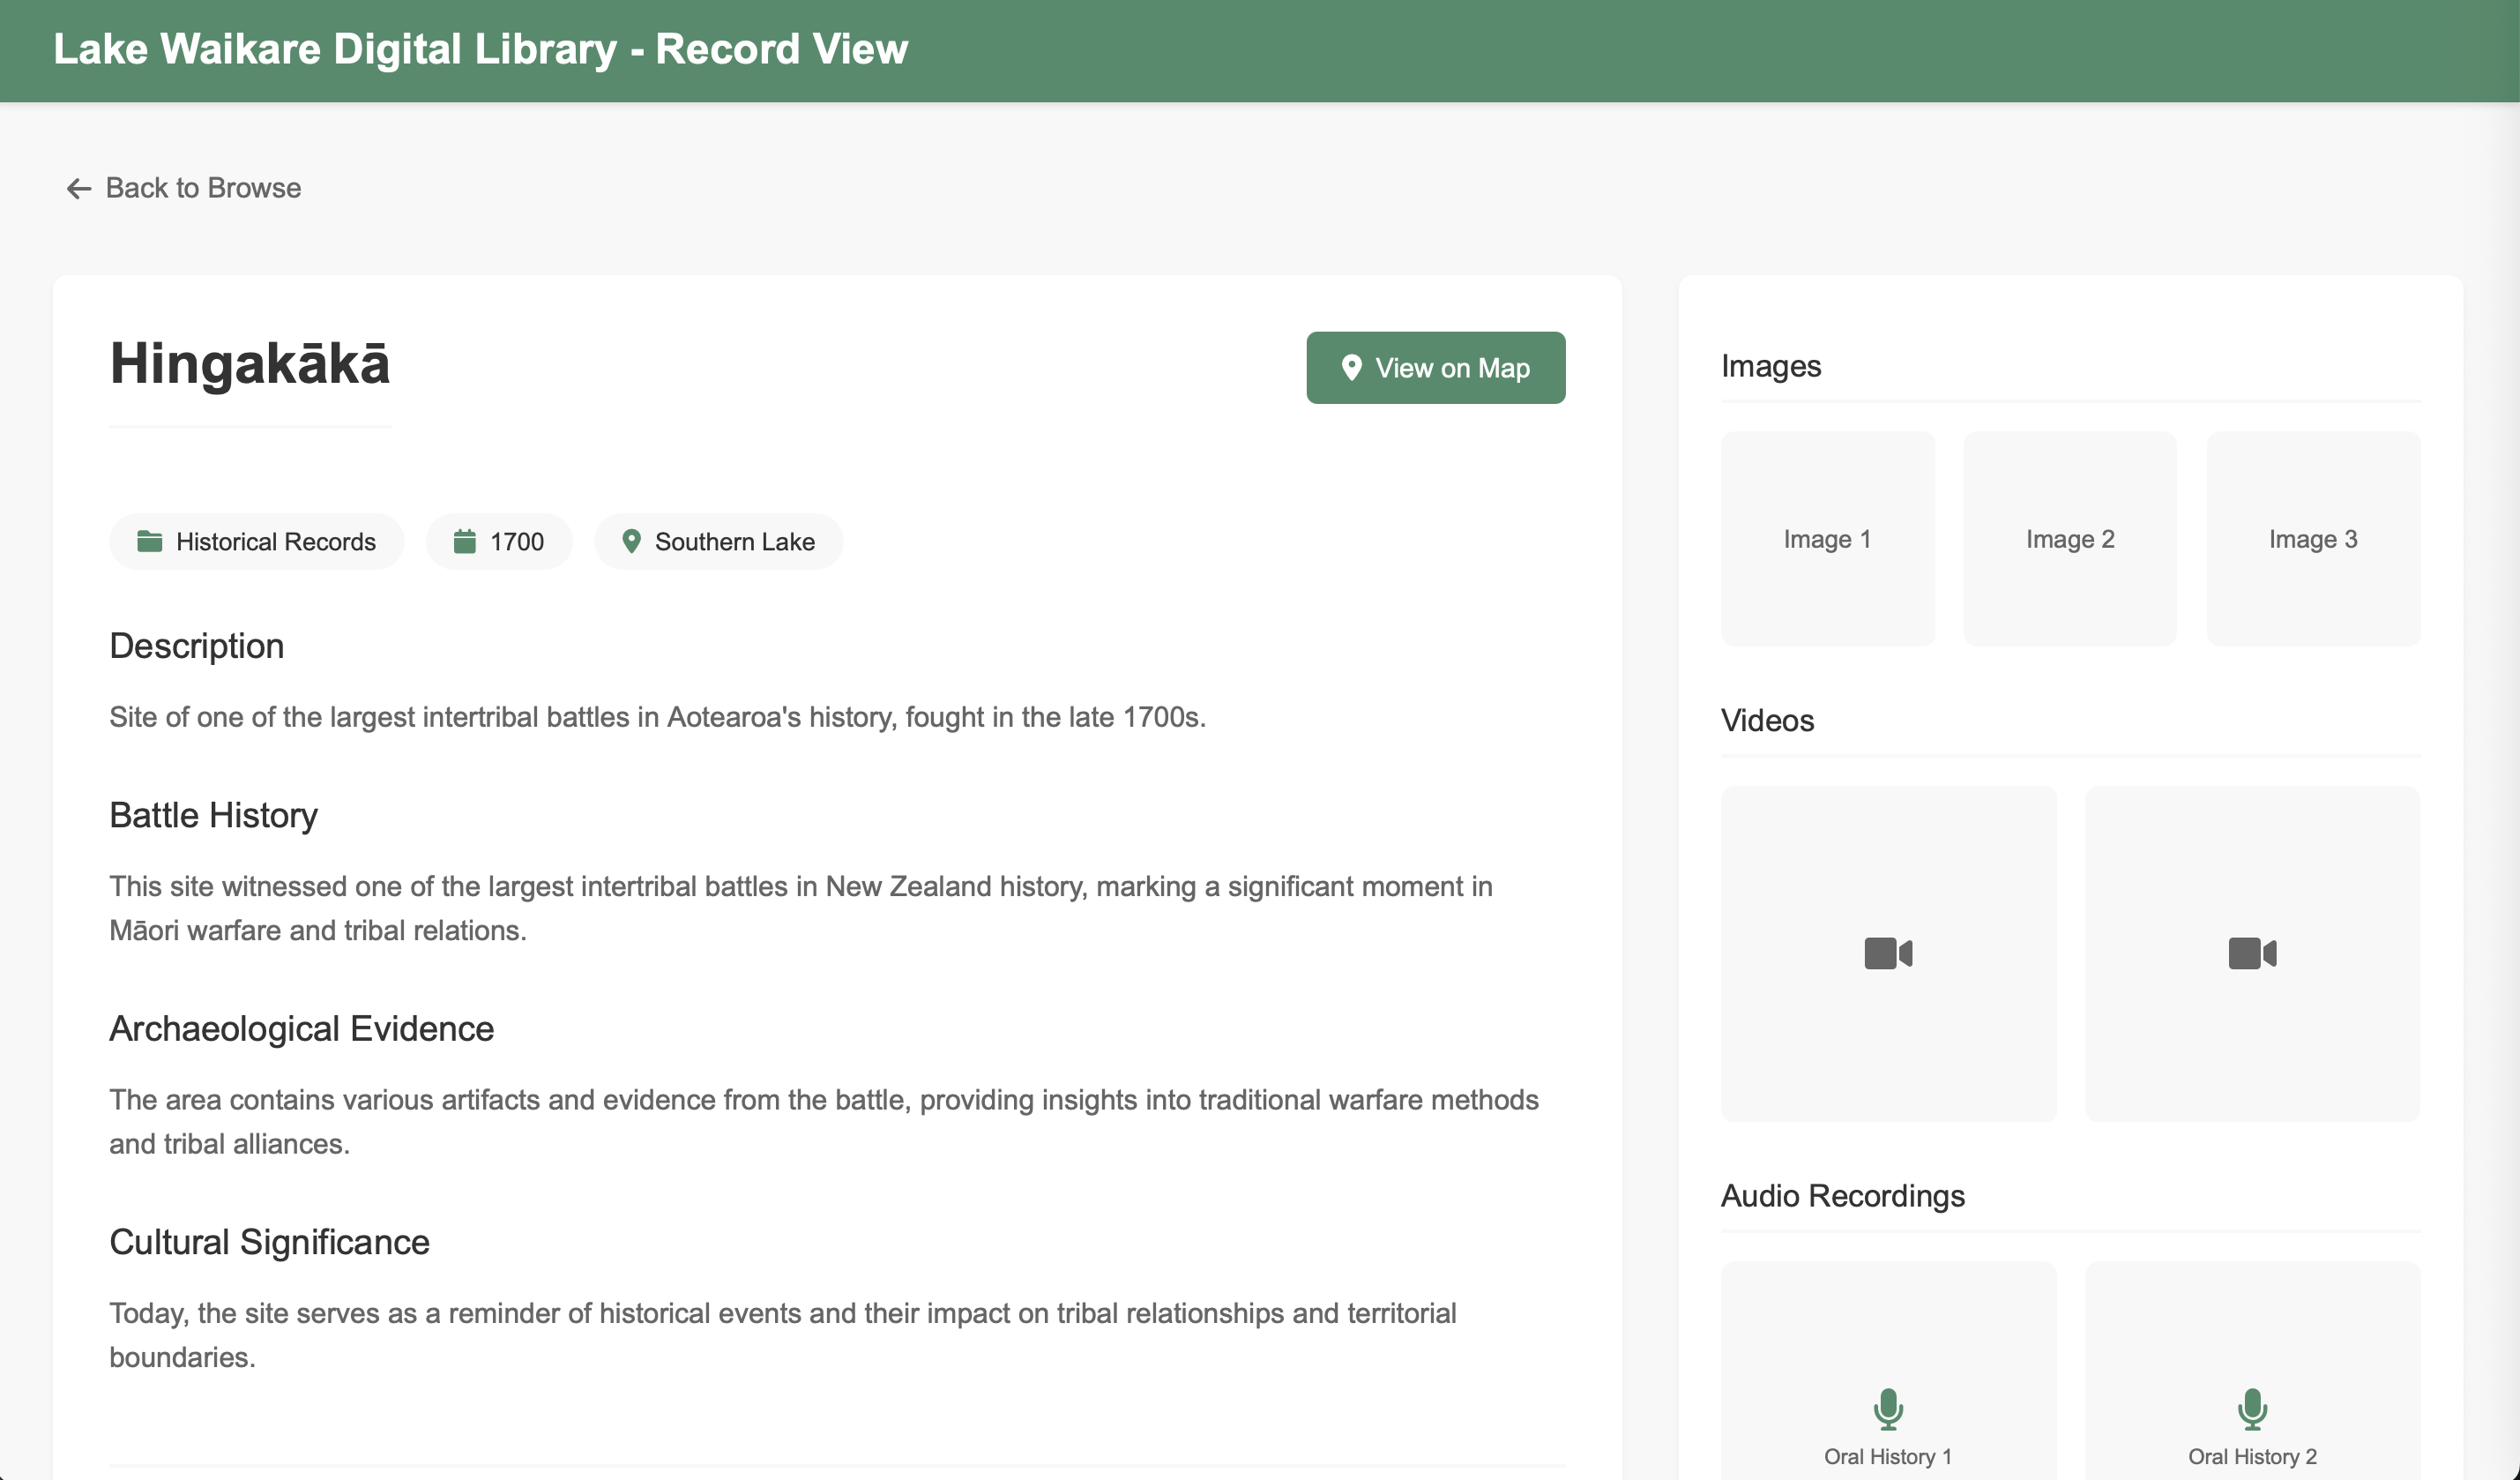
\includegraphics[width=\textwidth]{screenshot/prototype_single_record.png}
    \caption{Single Record}
  \end{subfigure}\hfill
  \begin{subfigure}[b]{0.3\textwidth}
    \includegraphics[width=\textwidth]{screenshot/prototype_main.png}
    \caption{Main}
  \end{subfigure}

  \caption{Prototype Stage Images}
  \label{fig:prototype}
\end{figure}



\end{document}